%%%%%%%%%%%%%%%%%%%%%%%%%%%%%%%%%%
% ICRA 2018 Submission Manuscript
% John Romanishin, John Mamish, and Daniela Rus
% SEPTEMBER 2017
%%%%%%%%%%%%%%%%%%%%%%%%%%%%%%%%%% 
   
\documentclass[letterpaper, 10 pt, conference]{ieeeconf}  
\IEEEoverridecommandlockouts  % This command is only needed if you
			      % want to use the \thanks command
\overrideIEEEmargins
% See the \addtolength command later in the file to balance the column lengths on the last page of the document
\ifx\pdfoutput\undefined

%%%%%%%%%%%%%%%%
%%% Packages %%%
%%%%%%%%%%%%%%%%

% we are running LaTeX, not pdflatex
\usepackage[dvips]{graphicx}
\else
% we are running pdflatex, so convert .eps files to .pdf
\usepackage[pdftex]{graphicx}
\usepackage{epstopdf}
\fi

\usepackage{amsmath, amssymb, mathptmx}
%\usepackage{algorithmic}
%\usepackage{algorithm}
\usepackage[linesnumbered, ruled]{algorithm2e}
\usepackage{multirow}
\usepackage{breakurl}
\usepackage{caption}
\usepackage{booktabs}
\usepackage{subcaption}
\usepackage[bookmarks=true,breaklinks=true,]{hyperref}

%%%  	 TIKZ 	  %%%

\usepackage{pgfplots}
\pgfplotsset{compat=1.7}
\usetikzlibrary{math} %needed tikz library
\usepackage{tikz-dimline}
\usepackage{tikz}
\usetikzlibrary{arrows,shapes,trees, fit}
\usetikzlibrary{calc,trees,positioning,arrows,chains,shapes.geometric,%
decorations.pathreplacing,decorations.pathmorphing,shapes,%
matrix,shapes.symbols,plotmarks,decorations.markings,shadows,arrows.meta,bending}


\definecolor{maroon}{RGB}{111,0,15}
\definecolor{light_orange}{RGB}{150,100,50}

%%%%%%%%%%%%%%%
%%%      Packages       %%%
%%%%%%%%%%%%%%%
\newcommand{\hvectspace}{\hspace{.2cm}}

%% Old Version \title{\LARGE \bf \TagNamePlural: Location specific tag}
\title{Three Fundamental Behaviors using Magnetic Barcodes on 3D M-Block System}

\author{John W. Romanishin, John Mamish, and Daniela Rus
  \thanks{J. W. Romanishin, D. Rus are with the Computer Science
    and Artificial Intelligence Lab, MIT, Cambridge, MA, 02139
    {\tt\small \{johnrom|rus\}@csail.mit.edu}.}
}


\begin{document}
	\newcounter{x}
	\newcounter{y}
	\newcounter{z}
	
\newcommand{\tagName}{mtag }
\newcommand{\TagName}{Mtag }
\newcommand{\tagNamePlural}{mtags}
\newcommand{\TagNamePlural}{Mtags}


\captionsetup[figure]{labelfont=small, textfont=small}
\captionsetup[table]{labelfont=small, textfont=small}

\maketitle
\thispagestyle{empty}
\pagestyle{empty}

%%%%%%%%%%%%%%%%%%
\begin{abstract}
%%%%%%%%%%%%%%%%%% 

This paper presents experimentally validated algorithms demonstrating three fundamental behaviors for lattice based Modular Self-Reconfigurable Robotic~(MSRR) modules utilizing a novel magnetic bar-code system to facilitate neighbor identification. For envisioned MSRR systems exceeding thousands of modules, centralized control of each robot movement will likely prove to be intractable from a computational and communication standpoint. An approach where individual modules can autonomously follow simple behaviors, while periodically accepting input from a centralized source promises to be simpler and more robust. This work presents three fundamental behaviors demonstrated with 3D M-Block modular robots. These behaviors include: (1) \textit{Path following} - modules guided to follow a three dimensional path based on passive magnetic fiducial tags (2) \textit{Line formation} - modules turning from arbitrary 3D structures into a line in an almost entirely decentralized control algorithm, and (3) \textit{Light gradient aggregation} - the formation of a large group of modules guided by a global stimulus i.e. visible light. These behaviors are implemented on 3D Mblock robotic modules, original described in~\cite{RomanishinRus-IROS13} and~\cite{Romanishin20153d} which have been outfitted with magnetic identification tags and electronics to read tags on each face. Using these tags, modules can accurately read passively stored information representing neighboring modules or messages encoded in magnetically signed tags. 
%%%%%%%%%%%%%%%%%%
\end{abstract}
%%%%%%%%%%%%%%%%%%

%%%%%%%%%%%%%%%%%%%%%%%%%
\section{Introduction}
\label{sec:Introduction}
%%%%%%%%%%%%%%%%%%%%%%%%%

Modular Self-Reconfigurable Robots (MSRR) have been proposed as one method of autonomously creating general purpose robotic systems of arbitrary complexity. MSRR systems generally can be thought of as consisting of individual \emph{modules}, which connect to either other active modules or passive modular elements through standardized \emph{connectors} to create specific \emph{configurations} in order to accomplish a designated task. Much of the existing work in the MSRR field has focused either on the preliminary development of novel hardware systems or general purpose algorithms which run on simulated systems. Few of the MSRR systems demonstrated to date have remained under active development long enough to develop and apply practical algorithms that can accomplish tasks using physical robots. This paper is focused on implementing and analyzing three separate practical partially decentralized "behaviors" with a set of 3D M-Block modules.

\newsavebox{\arrows}
\sbox{\arrows}
{
	\resizebox{1.4 in}{!}
	{
	\begin{tikzpicture}[x=(220:1cm), y=(-40:1cm), z=(90:0.707cm)]
		%%
%this code is from...
\setcounter{x}{0}%
\setcounter{y}{0}%
\setcounter{z}{0}%

% The angles of x,y,z-axes
\newcommand\xaxis{210}
\newcommand\yaxis{-30}
\newcommand\zaxis{90}

% The top side of a cube
\newcommand\topside[3]{
	\fill[fill=yellow, draw=black,shift={(\xaxis:#1)},shift={(\yaxis:#2)},
	shift={(\zaxis:#3)}] (0,0) -- (30:1) -- (0,1) --(150:1)--(0,0);
}

% The left side of a cube
\newcommand\leftside[3]{
	\fill[fill=red, draw=black,shift={(\xaxis:#1)},shift={(\yaxis:#2)},
	shift={(\zaxis:#3)}] (0,0) -- (0,-1) -- (210:1) --(150:1)--(0,0);
}

% The right side of a cube
\newcommand\rightside[3]{
	\fill[fill=blue, draw=black,shift={(\xaxis:#1)},shift={(\yaxis:#2)},
	shift={(\zaxis:#3)}] (0,0) -- (30:1) -- (-30:1) --(0,-1)--(0,0);
}

% The cube 
\newcommand\cube[3]{
	\topside{#1}{#2}{#3} \leftside{#1}{#2}{#3} \rightside{#1}{#2}{#3}
}

\newcommand\ArrowNE[3]
{
	\node at (#1+0.5, #2+0.5, #3) 
%	\node at (#1, #2, #3) 
	{
		\begin{tikzpicture}
		\draw[->, thick, >={Stealth[round]}, line width=0.4mm] (0.3,0) -- (-0.3,0);
		\end{tikzpicture}};
		
}

\newcommand\ArrowNL[3]
{
	\node at (#1+1, #2+0.5, #3-0.5) 
	%	\node at (#1, #2, #3) 
	{
		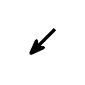
\begin{tikzpicture}
		\draw[->, thick, >={Stealth[round]}, line width=0.4mm] (0.16,0.16) -- (-0.16,-0.16);
		\end{tikzpicture}};
	
}

\newcommand\ArrowNR[3]
{
	\node at (#1+0.5, #2+1, #3-0.5) 
	%	\node at (#1, #2, #3) 
	{
		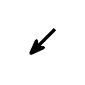
\begin{tikzpicture}
		\draw[->, thick, >={Stealth[round]}, line width=0.4mm] (0.16,0.16) -- (-0.16,-0.16);
		\end{tikzpicture}};
	
}

\newcommand\ArrowNW[3]
{
	\node at (#1+0.5, #2+0.5, #3) 
%	\node at (#1, #2, #3) 
	{
		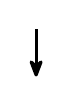
\begin{tikzpicture}
		\draw[->, thick, >={Stealth[round]}, line width=0.4mm] (0,0.3) -- (0,-0.3);
		\end{tikzpicture}};
	
}

\newcommand\ArrowSW[3]
{
	\node at (#1+0.5, #2+0.5, #3) 
%	\node at (#1, #2, #3) 
	{
		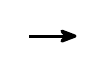
\begin{tikzpicture}
		\draw[<-, thick, >={Stealth[round]}, line width=0.4mm] (0.3,0) -- (-0.3,0);
		\end{tikzpicture}};
	
}

\newcommand\ArrowSE[3]
{
	\node at (#1+0.5, #2+0.5, #3) 
%	\node at (#1, #2, #3) 
	{
		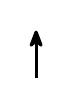
\begin{tikzpicture}
		\draw[<-, thick, >={Stealth[round]}, line width=0.4mm] (0,0.3) -- (0,-0.3);
		\end{tikzpicture}};
	
}

% Definition of \planepartition
% To draw the following plane partition, just write \planepartition{ {a, b, c}, {d,e} }.
%  a b c
%  d e
\newcommand\planepartition[1]{
	\setcounter{x}{-1}
	\foreach \a in {#1} {
		\addtocounter{x}{1}
		\setcounter{y}{-1}
		\foreach \b in \a {
			\addtocounter{y}{1}
			\setcounter{z}{-1}
			\foreach \c in {0,...,\b} {
				\addtocounter{z}{1}
				\ifthenelse{\c=0}{\setcounter{z}{-1},\addtocounter{y}{0}}{
					\cube{\value{x}}{\value{y}}{\value{z}}}
			}
		}
	}
}


%%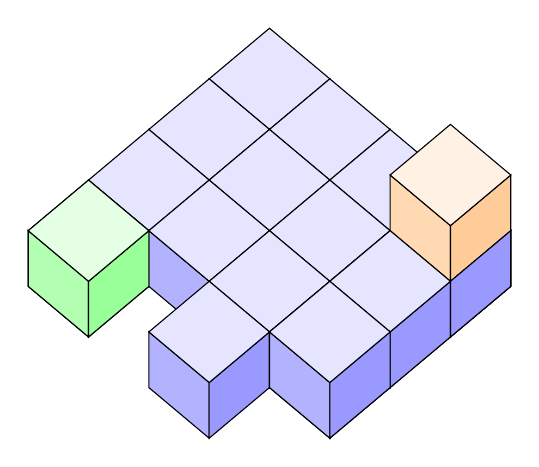
\begin{tikzpicture}[x=(220:1cm), y=(-40:1cm), z=(90:0.707cm)]
	%\planepartition{{0,0,1},{1,1,1},{1,0,0},{1,0,1}};
\foreach \m [count=\y] in {{1,1,1,1},{1,1,1},{1,1,1,1},{1,1,1}}{
	\foreach \n [count=\x] in \m {
		\ifnum \n>0
		\foreach \z in {1,...,\n}{
			\draw [fill=blue!30] (\x+1,\y,\z) -- (\x+1,\y+1,\z) -- (\x+1, \y+1, \z-1) -- (\x+1, \y, \z-1) -- cycle;
			\draw [fill=blue!40] (\x,\y+1,\z) -- (\x+1,\y+1,\z) -- (\x+1, \y+1, \z-1) -- (\x, \y+1, \z-1) -- cycle;
			\draw [fill=blue!10] (\x,\y,\z)   -- (\x+1,\y,\z)   -- (\x+1, \y+1, \z)   -- (\x, \y+1, \z) -- cycle;  
		}
	
		\fi
	}
}   

\foreach \m [count=\y] in {{0,0,0,1}, {0,0,0}} {
	\foreach \n [count=\x] in \m {
		\ifnum \n>0
		\foreach \z in {1,...,\n}{
			\draw [fill=green!30] (\x+1,\y,\z) -- (\x+1,\y+1,\z) -- (\x+1, \y+1, \z-1) -- (\x+1, \y, \z-1) -- cycle;
			\draw [fill=green!40] (\x,\y+1,\z) -- (\x+1,\y+1,\z) -- (\x+1, \y+1, \z-1) -- (\x, \y+1, \z-1) -- cycle;
			\draw [fill=green!10] (\x,\y,\z)   -- (\x+1,\y,\z)   -- (\x+1, \y+1, \z)   -- (\x, \y+1, \z) -- cycle;  
		}
		
		\fi
	}
}   

\ArrowNW{1}	{3}	{1};

\foreach \m [count=\y] in {{0,0,0,0},{0,0,0},{0,0,0,0},{2,0,0}}{
	\foreach \n [count=\x] in \m {
		\ifnum \n>0
		\foreach \z in {1,...,\n}{
			\draw [fill=orange!30] (\x+1,\y,\z) -- (\x+1,\y+1,\z) -- (\x+1, \y+1, \z-1) -- (\x+1, \y, \z-1) -- cycle;
			\draw [fill=orange!40] (\x,\y+1,\z) -- (\x+1,\y+1,\z) -- (\x+1, \y+1, \z-1) -- (\x, \y+1, \z-1) -- cycle;
			\draw [fill=orange!10] (\x,\y,\z)   -- (\x+1,\y,\z)   -- (\x+1, \y+1, \z)   -- (\x, \y+1, \z) -- cycle;  
		}
		
		\fi
	}
}  

\foreach \m [count=\y] in {{0},{0},{0},{0,1,1}}{
	\foreach \n [count=\x] in \m {
		\ifnum \n>0
		\foreach \z in {1,...,\n}{
			\draw [fill=blue!30] (\x+1,\y,\z) -- (\x+1,\y+1,\z) -- (\x+1, \y+1, \z-1) -- (\x+1, \y, \z-1) -- cycle;
			\draw [fill=blue!40] (\x,\y+1,\z) -- (\x+1,\y+1,\z) -- (\x+1, \y+1, \z-1) -- (\x, \y+1, \z-1) -- cycle;
			\draw [fill=blue!10] (\x,\y,\z)   -- (\x+1,\y,\z)   -- (\x+1, \y+1, \z)   -- (\x, \y+1, \z) -- cycle;  
		}
		
		\fi
	}
} 

\foreach \m [count=\y] in {{0},{0},{0},{1,0,0}}{
	\foreach \n [count=\x] in \m {
		\ifnum \n>0
		\foreach \z in {1,...,\n}{
		%	\draw [fill=blue!30] (\x+1,\y,\z) -- (\x+1,\y+1,\z) -- (\x+1, \y+1, \z-1) -- (\x+1, \y, \z-1) -- cycle;
			\draw [fill=blue!40] (\x,\y+1,\z) -- (\x+1,\y+1,\z) -- (\x+1, \y+1, \z-1) -- (\x, \y+1, \z-1) -- cycle;
		%	\draw [fill=blue!10] (\x,\y,\z)   -- (\x+1,\y,\z)   -- (\x+1, \y+1, \z)   -- (\x, \y+1, \z) -- cycle;  
		}
		
		\fi
	}
} 
		"x" "y" "z"

\ArrowNR{4} {1}	{1};
\ArrowNL{4} {1}	{1};

\ArrowNR{4} {3}	{1};
\ArrowNL{4} {3}	{1};

\ArrowNR{3} {4}	{1};
\ArrowNL{3} {4}	{1};

\ArrowNR{1} {4}	{1};
\ArrowNR{2} {4}	{1};

\ArrowNL{3} {2}	{1};

\ArrowSW{1}	{1}	{1};
\ArrowSW{2}	{1}	{1};
\ArrowSW{3}	{1}	{1};
\ArrowSW{4}	{1}	{1};


\ArrowNW{1}	{2}	{1};
\ArrowSW{2}	{2}	{1};
\ArrowNW{3}	{2}	{1};

\ArrowNW{2}	{3}	{1};
\ArrowNE{3}	{3}	{1};
\ArrowNE{4}	{3}	{1};

%\ArrowNW{1}	{4}	{1};
\ArrowSW{2}	{4}	{1};
\ArrowNW{3}	{4}	{1};
;
	\end{tikzpicture}
	}
}

\begin{figure}[t]
	\centering
	\begin{subfigure}[b]{1.6 in}
		%	\resizebox{.48\linewidth}{0.6 in}
		%	{
		\begin{tikzpicture}[]	
		\node at (0,0) {\includegraphics[width=.9\linewidth]{Figures/mTagsCover.png}};
		\node[opacity = 0.95, fill = white, rounded corners] at (-1.45,-1) {(a)};
		\end{tikzpicture}
		
		%	}
		%\subcaption{}
	\end{subfigure}
	~
	\begin{subfigure}[b]{0.48\linewidth}
	%	\resizebox{\linewidth}{!}
	%	{
		\begin{tikzpicture}[]
			\node at (0 cm, 0cm) {\usebox{\arrows}};
			\node[opacity = 0.95, fill = white, rounded corners] at (-1.5,-1.25) {(b)};
		\end{tikzpicture}
	%	}
	\end{subfigure}

	\begin{subfigure}[b]{\linewidth}
		\centering
		\begin{tikzpicture}[]	
		\node at (0,0) {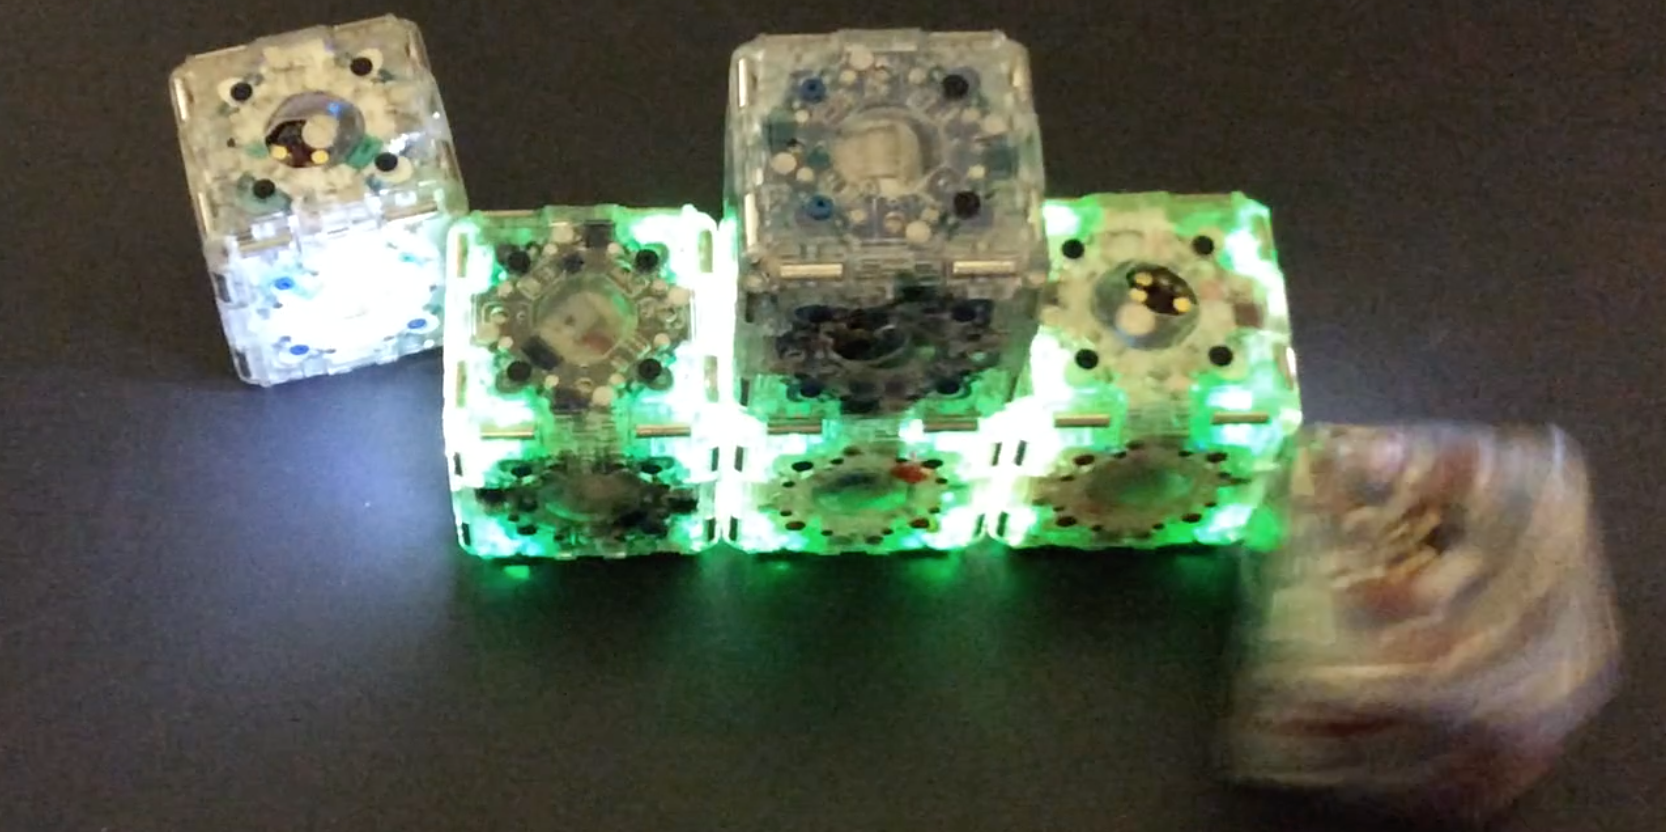
\includegraphics[width=.96\linewidth]{figures/ActualLine_3_small.png}};
		\node[opacity = 0.95, fill = white, rounded corners] at (-3.5,-1.75) {(c)};
		\end{tikzpicture}

	\end{subfigure}
	
	
	\caption{This figure illustrates several of the behaviors implemented with the 3D M-Blocks robots. (a) Shows a photo of an active module connected to a passive module which contains a Magnetic Fiducial with embedded orientation information. (b) Demonstrates an abstraction of the magnetic fiducials as "arrows" which a module implementing the path following behaviour would move along. In this example, the module shown in \emph{orange} would arrive on top of the \emph{green} module after successfully implementing the path following behavior. (c) Shows several modules implementing the line formation behavior.}
	
	\label{fig:intro}
\end{figure}

The conceptually simplest framework for controlling thousands or millions of individual modular robots is to have a centralized authority which dictates every move to each robot. However, centralized systems suffer from practical problems involved with maintaining the required number of communication links and in general lack robustness to disturbances and do not scale well. An alternative approach is to develop embedded "behaviors" or simple decentralized algorithms which each module can implement independently in the (potentially temporary) absence of centralized commutation. Several important characteristics that determine the possible complexity and effectiveness of potential behaviors include the type of sensor feedback, the (un)availability and type of local communication, and the systems' reconfiguration implementation. This work focuses on modules which have information only about their direct neighbors, global input from a stimulus source (i.e. visible light), knowledge about gravity, and occasional wireless communication with a higher level controller. The initial behaviors that we introduce include: (1) Path following, (2) Line formation, and (3) Light guided aggregation. The ability for a MSRR system to delegate many of the details of each module's movements to be autonomously implemented by the individual modules based on local information, while still allowing centralized control when necessary, improves the system's ability to scale effectivly to large systems. While there have been similar proposed decentralized control strategies, several of which are discussed in Section~\ref{ssec:RW-Algorithmic}, this work focuses on defining and adapting these behaviors for an existing robotic platform.

This work is implemented and experimentally validated through a set of twelve 3D M-Block modular robots; which are one of the few MSRR systems capable of three-dimensional reconfiguration according to a generalized 3D lattice reconfiguration model. These $50~mm$ cubic modules use pulses of angular momentum and temporary magnetic hinges in order to implement lattice reconfiguration according to the Pivoting Cube Model (PCM). The M-Blocks were introduced for 2D movement in 2013~\cite{RomanishinRus-IROS13} and extended to three dimensions in 2015~\cite{Romanishin20153d}. In order to facilitate the implementation of new primitive behaviors, the 3D M-Blocks are further extended in this work to include a novel type of magnetic fiducial which allows modules to detect information about their neighbors. These fiducial tags, called \tagNamePlural, provide globally unique identification codes for each face of a collection of modules. \TagNamePlural~include relative orientation of the connection between the reading module, and encode information passively, allowing the system to accurately determine its global configuration even when a fraction of modules are either disabled or are passive elements.

Specifically this paper presents the following technical contributions:
\begin{itemize}
	\item Developed and characterized a new type of magnetic fiducial (\TagNamePlural) specifically designed to address the task of neighbor identification and determining connection orientation for MSRR. (Section~\ref{sec:Hardware})
	\item Defined three separate primitive MSRR behaviors tailored for the 3D M-Block hardware system. (Section~\ref{sec:Behaviors})
	\item Experimentally validated these behaviors on a system of twelve 3D M-Block modules. (Section~\ref{sec:Experiments})
\end{itemize}

%The remainder of the paper is organized as follows: Section~\ref{sec:RelatedWork} gives an overview of related work that pertains to modular robots with a focus on how existing %MSRR systems identify and encode physical configuration information through their connectors. Next, Section~\ref{sec:Hardware} presents the technical details of the proposed %\tagNamePlural~system for determining neighbor connection information and then attempts to characterize their functionality and discusses current limitations and potential %future extensions. Next, Section ~\ref{sec:Behaviors} presents the detailed algorithms which implement the three behaviors, (1) Path following: (2) Line formation and (3) Light %Aggregation, while Section~\ref{sec:Experiments} presents and analyzes experiments implementing these three algorithms. Finally, Section~\ref{sec:Discussion} attempts to help %illustrate several of the challenges and requirements for eventually applying these behaviors to future systems with millions of modules.


%\begin{figure}[htb]
%
%	%%
%this code is from...
\setcounter{x}{0}%
\setcounter{y}{0}%
\setcounter{z}{0}%

% The angles of x,y,z-axes
\newcommand\xaxis{210}
\newcommand\yaxis{-30}
\newcommand\zaxis{90}

% The top side of a cube
\newcommand\topside[3]{
	\fill[fill=yellow, draw=black,shift={(\xaxis:#1)},shift={(\yaxis:#2)},
	shift={(\zaxis:#3)}] (0,0) -- (30:1) -- (0,1) --(150:1)--(0,0);
}

% The left side of a cube
\newcommand\leftside[3]{
	\fill[fill=red, draw=black,shift={(\xaxis:#1)},shift={(\yaxis:#2)},
	shift={(\zaxis:#3)}] (0,0) -- (0,-1) -- (210:1) --(150:1)--(0,0);
}

% The right side of a cube
\newcommand\rightside[3]{
	\fill[fill=blue, draw=black,shift={(\xaxis:#1)},shift={(\yaxis:#2)},
	shift={(\zaxis:#3)}] (0,0) -- (30:1) -- (-30:1) --(0,-1)--(0,0);
}

% The cube 
\newcommand\cube[3]{
	\topside{#1}{#2}{#3} \leftside{#1}{#2}{#3} \rightside{#1}{#2}{#3}
}

\newcommand\ArrowNE[3]
{
	\node at (#1+0.5, #2+0.5, #3) 
%	\node at (#1, #2, #3) 
	{
		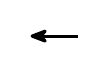
\begin{tikzpicture}
		\draw[->, thick, >={Stealth[round]}, line width=0.4mm] (0.3,0) -- (-0.3,0);
		\end{tikzpicture}};
		
}

\newcommand\ArrowNL[3]
{
	\node at (#1+1, #2+0.5, #3-0.5) 
	%	\node at (#1, #2, #3) 
	{
		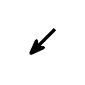
\begin{tikzpicture}
		\draw[->, thick, >={Stealth[round]}, line width=0.4mm] (0.16,0.16) -- (-0.16,-0.16);
		\end{tikzpicture}};
	
}

\newcommand\ArrowNR[3]
{
	\node at (#1+0.5, #2+1, #3-0.5) 
	%	\node at (#1, #2, #3) 
	{
		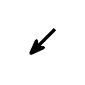
\begin{tikzpicture}
		\draw[->, thick, >={Stealth[round]}, line width=0.4mm] (0.16,0.16) -- (-0.16,-0.16);
		\end{tikzpicture}};
	
}

\newcommand\ArrowNW[3]
{
	\node at (#1+0.5, #2+0.5, #3) 
%	\node at (#1, #2, #3) 
	{
		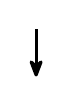
\begin{tikzpicture}
		\draw[->, thick, >={Stealth[round]}, line width=0.4mm] (0,0.3) -- (0,-0.3);
		\end{tikzpicture}};
	
}

\newcommand\ArrowSW[3]
{
	\node at (#1+0.5, #2+0.5, #3) 
%	\node at (#1, #2, #3) 
	{
		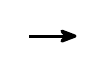
\begin{tikzpicture}
		\draw[<-, thick, >={Stealth[round]}, line width=0.4mm] (0.3,0) -- (-0.3,0);
		\end{tikzpicture}};
	
}

\newcommand\ArrowSE[3]
{
	\node at (#1+0.5, #2+0.5, #3) 
%	\node at (#1, #2, #3) 
	{
		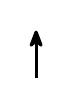
\begin{tikzpicture}
		\draw[<-, thick, >={Stealth[round]}, line width=0.4mm] (0,0.3) -- (0,-0.3);
		\end{tikzpicture}};
	
}

% Definition of \planepartition
% To draw the following plane partition, just write \planepartition{ {a, b, c}, {d,e} }.
%  a b c
%  d e
\newcommand\planepartition[1]{
	\setcounter{x}{-1}
	\foreach \a in {#1} {
		\addtocounter{x}{1}
		\setcounter{y}{-1}
		\foreach \b in \a {
			\addtocounter{y}{1}
			\setcounter{z}{-1}
			\foreach \c in {0,...,\b} {
				\addtocounter{z}{1}
				\ifthenelse{\c=0}{\setcounter{z}{-1},\addtocounter{y}{0}}{
					\cube{\value{x}}{\value{y}}{\value{z}}}
			}
		}
	}
}


%%\begin{tikzpicture}[x=(220:1cm), y=(-40:1cm), z=(90:0.707cm)]
	%\planepartition{{0,0,1},{1,1,1},{1,0,0},{1,0,1}};
\foreach \m [count=\y] in {{1,1,1,1},{1,1,1},{1,1,1,1},{1,1,1}}{
	\foreach \n [count=\x] in \m {
		\ifnum \n>0
		\foreach \z in {1,...,\n}{
			\draw [fill=blue!30] (\x+1,\y,\z) -- (\x+1,\y+1,\z) -- (\x+1, \y+1, \z-1) -- (\x+1, \y, \z-1) -- cycle;
			\draw [fill=blue!40] (\x,\y+1,\z) -- (\x+1,\y+1,\z) -- (\x+1, \y+1, \z-1) -- (\x, \y+1, \z-1) -- cycle;
			\draw [fill=blue!10] (\x,\y,\z)   -- (\x+1,\y,\z)   -- (\x+1, \y+1, \z)   -- (\x, \y+1, \z) -- cycle;  
		}
	
		\fi
	}
}   

\foreach \m [count=\y] in {{0,0,0,1}, {0,0,0}} {
	\foreach \n [count=\x] in \m {
		\ifnum \n>0
		\foreach \z in {1,...,\n}{
			\draw [fill=green!30] (\x+1,\y,\z) -- (\x+1,\y+1,\z) -- (\x+1, \y+1, \z-1) -- (\x+1, \y, \z-1) -- cycle;
			\draw [fill=green!40] (\x,\y+1,\z) -- (\x+1,\y+1,\z) -- (\x+1, \y+1, \z-1) -- (\x, \y+1, \z-1) -- cycle;
			\draw [fill=green!10] (\x,\y,\z)   -- (\x+1,\y,\z)   -- (\x+1, \y+1, \z)   -- (\x, \y+1, \z) -- cycle;  
		}
		
		\fi
	}
}   

\ArrowNW{1}	{3}	{1};

\foreach \m [count=\y] in {{0,0,0,0},{0,0,0},{0,0,0,0},{2,0,0}}{
	\foreach \n [count=\x] in \m {
		\ifnum \n>0
		\foreach \z in {1,...,\n}{
			\draw [fill=orange!30] (\x+1,\y,\z) -- (\x+1,\y+1,\z) -- (\x+1, \y+1, \z-1) -- (\x+1, \y, \z-1) -- cycle;
			\draw [fill=orange!40] (\x,\y+1,\z) -- (\x+1,\y+1,\z) -- (\x+1, \y+1, \z-1) -- (\x, \y+1, \z-1) -- cycle;
			\draw [fill=orange!10] (\x,\y,\z)   -- (\x+1,\y,\z)   -- (\x+1, \y+1, \z)   -- (\x, \y+1, \z) -- cycle;  
		}
		
		\fi
	}
}  

\foreach \m [count=\y] in {{0},{0},{0},{0,1,1}}{
	\foreach \n [count=\x] in \m {
		\ifnum \n>0
		\foreach \z in {1,...,\n}{
			\draw [fill=blue!30] (\x+1,\y,\z) -- (\x+1,\y+1,\z) -- (\x+1, \y+1, \z-1) -- (\x+1, \y, \z-1) -- cycle;
			\draw [fill=blue!40] (\x,\y+1,\z) -- (\x+1,\y+1,\z) -- (\x+1, \y+1, \z-1) -- (\x, \y+1, \z-1) -- cycle;
			\draw [fill=blue!10] (\x,\y,\z)   -- (\x+1,\y,\z)   -- (\x+1, \y+1, \z)   -- (\x, \y+1, \z) -- cycle;  
		}
		
		\fi
	}
} 

\foreach \m [count=\y] in {{0},{0},{0},{1,0,0}}{
	\foreach \n [count=\x] in \m {
		\ifnum \n>0
		\foreach \z in {1,...,\n}{
		%	\draw [fill=blue!30] (\x+1,\y,\z) -- (\x+1,\y+1,\z) -- (\x+1, \y+1, \z-1) -- (\x+1, \y, \z-1) -- cycle;
			\draw [fill=blue!40] (\x,\y+1,\z) -- (\x+1,\y+1,\z) -- (\x+1, \y+1, \z-1) -- (\x, \y+1, \z-1) -- cycle;
		%	\draw [fill=blue!10] (\x,\y,\z)   -- (\x+1,\y,\z)   -- (\x+1, \y+1, \z)   -- (\x, \y+1, \z) -- cycle;  
		}
		
		\fi
	}
} 
		"x" "y" "z"

\ArrowNR{4} {1}	{1};
\ArrowNL{4} {1}	{1};

\ArrowNR{4} {3}	{1};
\ArrowNL{4} {3}	{1};

\ArrowNR{3} {4}	{1};
\ArrowNL{3} {4}	{1};

\ArrowNR{1} {4}	{1};
\ArrowNR{2} {4}	{1};

\ArrowNL{3} {2}	{1};

\ArrowSW{1}	{1}	{1};
\ArrowSW{2}	{1}	{1};
\ArrowSW{3}	{1}	{1};
\ArrowSW{4}	{1}	{1};


\ArrowNW{1}	{2}	{1};
\ArrowSW{2}	{2}	{1};
\ArrowNW{3}	{2}	{1};

\ArrowNW{2}	{3}	{1};
\ArrowNE{3}	{3}	{1};
\ArrowNE{4}	{3}	{1};

%\ArrowNW{1}	{4}	{1};
\ArrowSW{2}	{4}	{1};
\ArrowNW{3}	{4}	{1};

%
%	\caption{large structure}
%
%	\label{fig:cover2}
%\end{figure}
%
%\begin{figure}[htb]
%
%  \centering
%  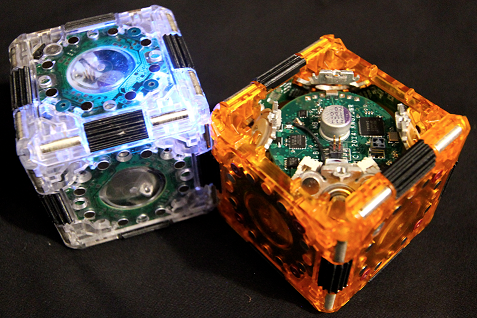
\includegraphics[width=3.4in]{Figures/cover.png}
%
%  \caption{M-Bocks modular robots with connections illuminated with onboard LEDs}
%
%  \label{fig:cover}
%\end{figure}


\section{Related Work}
\label{sec:RelatedWork}

Many papers that provide a comprehensive overviews of the field of modular robotics including work up to 2007~[cite to do], and several updates more recently ~[cite to do], and ~[cite to do] which provides a good background on connectors. This section of the paper will attempt to investigate two different topics in the related work in a more focues manner, Sec~\label{sec:RWconfiguration} will look at the challenge of configuration discovery in modular robotics systems, and~\label{sec:RWtaggingTech} will compare and contrast different technologies for location specific tagging tagging technologies.


\subsection{Modular Robots Overview}
\label{sec:RWconfiguration}
	The ability for a modular system to discover the specific configuration of modules at any and all times is one of the most essential tasks for any modular robotic system. However, many of the modular robotic systems proposed to date have either built very limited and error prone methods for solving this problem, or have ommited implementation of such a system entirely. Any \textbf{connection} between modules in a modular system involves a minimium of three unique parameters 1) Some form of Identity or \textbf{ID} of the two modules in question, 2) the connector, or \textbf{face number} for each of the modules, and 3) the \textbf{orientation} of the connection, which in a cubic lattice is one of four possible 90 degree values.
		
	Many of the existing systems have faces which are able to pass information locally. This communication be used to discover the face number and the module ID's, but we are not aware of any of these systems which are able to systematically disover the orientation of the connection. Many of these systems seem to rely on using the face-to-face connection combined with inertial measurement sensors in order to construct the 
	
	Two of the most problematic aspects of current systems we have identified are the need for both modules involed to be activly . lack of robust connector orientation information
	Many differnt systems, including the pebbles[cite], smores[cite]... While there are 

	

\subsection{Location Tagging technology overview}
\label{sec:RWtaggingTech}

There are several different types of passive tagging technologies designed allow the recognization of tags. These include RFID, NFC, QR-Codes, April Tags, etc... 


\begin{table*}[t]
	\centering
	\caption{Comparison of attributes for several various tagging technologies}
	\newcommand{\wdd}{1.8cm}
	\begin{tabular}{ p{\wdd} |p{\wdd}  p{\wdd} p{\wdd} p{\wdd} p{\wdd} p{\wdd} p{\wdd}  }
		\hline
		%1 - EMPTY
		& RFID 				%2
		& Light Based		%3
		& NFC Tags 			%4
		& Electrical 		%5s
		& QR Codes 			%6
		& Barcodes			%7
		& \tagNamePlural \\ %8
		\hline
		%%		   			RFID		LIGHT		NFC		   ELEC					QR		
		%%		1			2		3			4			5						6			7		8
		Short Description		& uses radio waves	& 			& 			& 					& 			& 	  	& Measure field direction of permanant magnets \\
		
		Cost			& Expensive	& expensive	& 			& 					& 			& 	  	& Inexpensive \\
		Standard		& 			&  			& Priprietary	& 					& 			& 	  						& Open \\
		Size 			& significant & minimal & tags  	& minimal	  				&       	&     	& Small		  \\
		Passive 		& yes		& 			&  			&	 				&			& 		& yes!		  \\
		Orientation 	& req. 4+ tags 		& possible 	& req. 4+ tags 	&	 				&	  		& 		& yes!		\\
		Modular Robots 	& [cite]	& yes		&	  		&					& yes, [..]	& 		& 3D M-Blocks\\
		Range			& 0-10$m$	& variable	& 0-6 mm	& physical contact	& varies	&		& 0-1$mm$	\\
	\end{tabular}	
	\label{tab:tagTech}    
\end{table*}


\section{Hardware}
\label{sec:Hardware}

\newsavebox{\faceDiagram}
\sbox{\faceDiagram}	{
	\newcommand{\statcirc}[4]{
	\fill[opacity = 0.5, red,shift={(#1 cm,#2 cm)}, rotate=#3] (0,0) circle (#4); 
	\fill[opacity = 0.5, blue,shift={(#1 cm,#2 cm)},rotate=#3] (0,0) -- (180:#4) arc (180:0:#4) -- cycle;
	%	\draw[->,black,shift={(#1 cm,#2 cm)},rotate=#3] (#4, 0)
}

\newcommand{\drawArrow}[3]{
	\draw[->,>={Stealth[round]}, line width=0.75mm, black ,shift={(#1 cm,#2 cm)}, rotate=#3] (0,-0.5) -- (0,0.5); 
}

\newcommand{\drawchip}[3]{
	\tikzmath
	{
		\chipW = 0.35;
		\chipH = 0.4;
	}
	\fill[opacity = 0.75, darkgray, shift= {(#1 cm, #2 cm)}, rotate = #3, rounded corners] (-\chipH,-\chipW) rectangle (\chipH,\chipW);
	\fill[orange,shift= {(#1 cm, #2 cm)}, rotate = #3 ] (-0.25,0.2) circle (0.1);
}
\begin{tikzpicture}

	\tikzmath{
		\offsetAxis = 0.5;
		\offsetCent = 2.9;
		\diameter = 0.32;
	}
	\draw node (A) at (-0.5, 1.7) {};
	\draw node (B) at (0, 1.7) {};
	\drawchip{\offsetAxis}{\offsetCent}{0};
	\drawchip{-\offsetAxis}{-\offsetCent}{180};
	
	%Magnet North
	\statcirc{-\offsetAxis}{\offsetCent}{70}{\diameter};
	
	\drawArrow{-\offsetAxis}{\offsetCent}{70}
	
	%Magnet EAST
	\statcirc{\offsetCent}{\offsetAxis}{20}{\diameter};
	
	% Magnet West
	\statcirc{\offsetAxis}{-\offsetCent}{190}{\diameter};
	
	\statcirc{-\offsetCent}{-\offsetAxis}{45}{\diameter};
	
	\draw[gray, dashed] (-\offsetAxis,{\offsetCent + 1}) -- 
	(-\offsetAxis,{\offsetCent - 1});
	\draw[black,dotted] (0,0) circle (2.95);
	
	% 4 Cross Lines X
	\draw[black,dashed] (0,0) -- (4,0);
	\draw[black,dashed] (0,0) -- (-4,0);
	\draw[black,dashed] (0,0) -- (0,4);
	\draw[black,dashed] (0,0) -- (0,-4);
	
%	\draw[purple, dotted] ()
	% Dimensioned Variables
	\dimline[line style = {line width = 0.8, arrows = dimline reverse-dimline reverse}] {(A)}{(B)}{x};
	
	% Arc Radius
	\dimline[line style = {line width = 0.8}] {(0,0)} {++(150:2.95)}{R};
%	\dimline {(1,0)}{(-1,0)}{x};
\end{tikzpicture}
}

\newsavebox{\magnetDigitization}
\sbox{\magnetDigitization}	{
	
\newcommand{\statcirc}[4]{
	\fill[red,shift={(#1 cm,#2 cm)}, rotate=#3] (0,0) circle (#4); 
	\fill[blue,shift={(#1 cm,#2 cm)},rotate=#3] (0,0) -- (180:#4) arc (180:0:#4) -- cycle;
	%	\draw[->,black,shift={(#1 cm,#2 cm)},rotate=#3] (#4, 0)
}

\newcommand{\drawArrow}[3]{
	\draw[->,>={Stealth[round]}, line width=0.75mm, black ,shift={(#1 cm,#2 cm)}, rotate=#3] (0,-1) -- (0,1); 
}

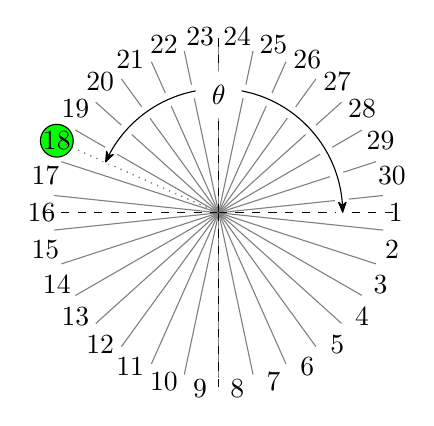
\begin{tikzpicture}[scale = 0.75]
\tikzmath{
	\offsetAxis = 0.5;
	\offsetCent = 2.9;
	\diameter = 0.75;
}

\foreach \i in {1,...,30}
{
	\draw[gray] (0,0) -- (\i * 12-6 : 2.8);
	\node[inner sep=0pt] at (-{\i * 12}+12: 3) {\i};
}
\node[circle,draw,inner sep=0pt, fill = green] at (-{18 * 12}+12: 3) {18};
\statcirc{0}{0}{-204-90}{\diameter};
\drawArrow{0}{0}{-204-90};
\draw[black,dashed] (0,0) -- (3,0);
\draw[black,dashed] (0,0) -- (-3,0);
\draw[black,dashed] (0,0) -- (0,3);
\draw[black,dashed] (0,0) -- (0,-3);
\draw[gray, dotted] (0,0) -- (-204: 3);
\draw[gray, dotted] (0,0) -- (-204: 3);
\draw [white, line width = 5pt] (2.1,0)  arc (0:360-204:2.1);
\draw [<->, >={Stealth[round]}] (2.1,0)  arc (0:360-204:2.1);
\node[circle,inner sep=3pt, fill = white]				at (90:2) {$\theta$};
\end{tikzpicture}
}

%%%%%%%%%%%%%%%%%%%%
The \tagNamePlural were designed and tested with the M-Blocks modular robots as the test bed, although nothing precludes their use in other circumstances. In this section we breifly describe the M-Blocks hardware, and then describe the mechanical, and electrical aspects of the new \tagNamePlural.

\subsection{M-Blocks hardware overview}
\label{sec:mblocksOverview}

The \tagName were designed and tested with the M-Blocks modular robots as the test bed, although nothing precludes their use in other circumstances and [], called the 3d M-Blocks. Characteristics of the M-Blocks at a glance can be seen in Table~\ref{tab:hardwareOverview}

\subsection{\tagNamePlural Hardware Overview}
\label{sec:tagsOverview}
In order to create a tag where the reader and the tag are both ungendered...


\begin{figure*}[t]
	%\begin{tikzpicture}[minimum width = 14 cm, minimum height = 6 cm]
		%\draw (0,0) -- (14,6);
		
		\begin{tikzpicture}[]
		%complexnode/.pic={\usebox{\mybox}}]

		\newcommand\xa{2};
		\newcommand\xb{2};
		\newcommand\ya{2};
		\newcommand\yb{2};
		
		\coordinate (smallNE) at (2,5);
		\coordinate (smallSE) at (2,5);
		\coordinate (smallSW) at (2,5);
		\coordinate (smallNW) at (2,5);
		
		\coordinate (bigNE) at (2,5);
		\coordinate (bigSE) at (2,5);
		\coordinate (bigSW) at (2,5);
		\coordinate (bigSE) at (2,5);
		
		\node at (4 cm, 4 cm) {\usebox{\faceDiagram}};
		\node at (10 cm, 6 cm) {\usebox{\magnetDigitization}};
	
		
		%\draw (1,1) pic {complexnode} (4,4);
		
		\end{tikzpicture}
	%%%%%%%%%%%%%%%%%%%%%%%%%%%%%%%%%%%%%%%%%%%%
	\caption{TEXT GOES HERE $\pi$ /2 4 way symmetric layout}
	\label{fig:tagDiagram8}
\end{figure*}


%\begin{figure}[b]
%%%%%%%%%%%%%%%%%%%%%%%%%%%%%%%%%%%%%%%%%%%%%
%	
\newcommand{\statcirc}[4]{
	\fill[red,shift={(#1 cm,#2 cm)}, rotate=#3] (0,0) circle (#4); 
	\fill[blue,shift={(#1 cm,#2 cm)},rotate=#3] (0,0) -- (180:#4) arc (180:0:#4) -- cycle;
	%	\draw[->,black,shift={(#1 cm,#2 cm)},rotate=#3] (#4, 0)
}

\newcommand{\drawArrow}[3]{
	\draw[->,>={Stealth[round]}, line width=0.75mm, black ,shift={(#1 cm,#2 cm)}, rotate=#3] (0,-0.5) -- (0,0.5); 


}

\newcommand{\drawchip}[3]{
	\tikzmath
	{
		\chipW = 0.35;
		\chipH = 0.4;
	}
	\fill[ black, shift= {(#1 cm, #2 cm)}, rotate = #3 ] (-\chipH,-\chipW) rectangle (\chipH,\chipW);
	\fill[ orange,shift= {(#1 cm, #2 cm)}, rotate = #3 ] (-0.25,0.25) circle (0.125);
	
}

\begin{tikzpicture}
\tikzmath{
	\offsetAxis = 0.5;
	\offsetCent = 2.9;
	\diameter = 0.32;
}

\drawchip{\offsetAxis}{\offsetCent}{0};
\drawchip{-\offsetAxis}{-\offsetCent}{180};
\statcirc{-\offsetAxis}{\offsetCent}{30}{\diameter};
\drawArrow{-\offsetAxis}{\offsetCent}{30}
\statcirc{\offsetCent}{\offsetAxis}{210}{\diameter};
\statcirc{\offsetAxis}{-\offsetCent}{190}{\diameter};
\statcirc{-\offsetCent}{-\offsetAxis}{45}{\diameter};
\draw[gray, dashed] (-\offsetAxis,{\offsetCent + 1}) -- 
(-\offsetAxis,{\offsetCent - 1});
\draw[black,dotted] (0,0) circle (3);
\draw[black,dashed] (0,0) -- (4,0);
\draw[black,dashed] (0,0) -- (-4,0);
\draw[black,dashed] (0,0) -- (0,4);
\draw[black,dashed] (0,0) -- (0,-4);
\end{tikzpicture}
%%%%%%%%%%%%%%%%%%%%%%%%%%%%%%%%%%%%%%%%%%%%%
%	\caption{tags consist of 4 diametrically magnetized
%	magnes arranged in a $\pi$ /2 4 way symmetric layout}
%	\label{fig:tagDiagram}
%\end{figure}

%\begin{figure}[b]
%	%%%%%%%%%%%%%%%%%%%%%%%%%%%%%%%%%%%%%%%%%%%%
%	
\newcommand{\statcirc}[4]{
	\fill[red,shift={(#1 cm,#2 cm)}, rotate=#3] (0,0) circle (#4); 
	\fill[blue,shift={(#1 cm,#2 cm)},rotate=#3] (0,0) -- (180:#4) arc (180:0:#4) -- cycle;
	%	\draw[->,black,shift={(#1 cm,#2 cm)},rotate=#3] (#4, 0)
}

\newcommand{\drawArrow}[3]{
	\draw[->,>={Stealth[round]}, line width=0.75mm, black ,shift={(#1 cm,#2 cm)}, rotate=#3] (0,-1) -- (0,1); 
}

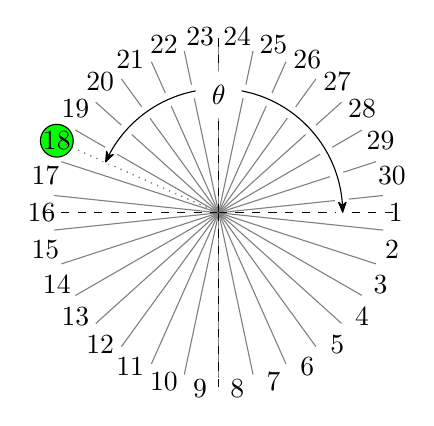
\begin{tikzpicture}[scale = 0.75]
\tikzmath{
	\offsetAxis = 0.5;
	\offsetCent = 2.9;
	\diameter = 0.75;
}

\foreach \i in {1,...,30}
{
	\draw[gray] (0,0) -- (\i * 12-6 : 2.8);
	\node[inner sep=0pt] at (-{\i * 12}+12: 3) {\i};
}
\node[circle,draw,inner sep=0pt, fill = green] at (-{18 * 12}+12: 3) {18};
\statcirc{0}{0}{-204-90}{\diameter};
\drawArrow{0}{0}{-204-90};
\draw[black,dashed] (0,0) -- (3,0);
\draw[black,dashed] (0,0) -- (-3,0);
\draw[black,dashed] (0,0) -- (0,3);
\draw[black,dashed] (0,0) -- (0,-3);
\draw[gray, dotted] (0,0) -- (-204: 3);
\draw[gray, dotted] (0,0) -- (-204: 3);
\draw [white, line width = 5pt] (2.1,0)  arc (0:360-204:2.1);
\draw [<->, >={Stealth[round]}] (2.1,0)  arc (0:360-204:2.1);
\node[circle,inner sep=3pt, fill = white]				at (90:2) {$\theta$};
\end{tikzpicture}
%	%%%%%%%%%%%%%%%%%%%%%%%%%%%%%%%%%%%%%%%%%%%%
%	\caption{tags consist of 4 diametrically magnetized
%		magnets arranged in a $\pi$/2 4 way symmetric layout}
%	\label{fig:tagDiagram}
%\end{figure}

\begin{table}[b]
  \caption{Basic info of the m-Blocks modular robots}

  \begin{tabular}{ p{3.4cm}  p{1.9cm} }
    \hline
    Actuation Directions & 6 \\
    Mass  & 150\,g \\
    Characterist Dimension & 50\,mm \\dra
    Total Parts  & 216 \\
    Actuated Moving Parts  & 10 \\
    Est. Cost & \$130 \\

  \end{tabular}

    \label{tab:hardwareOverview}
\end{table}


\subsection{Magnetic Barcodes Overview}
\label{sec:FlywheelAndBraking}

Several different Tag technologies are shown in Table~\ref{tab:info}.

More Text


%\begin{figure}[H]
%	\begin{tikzpicture}
%   	 \node[anchor=south west, inner sep=0] (image) at (0,0) {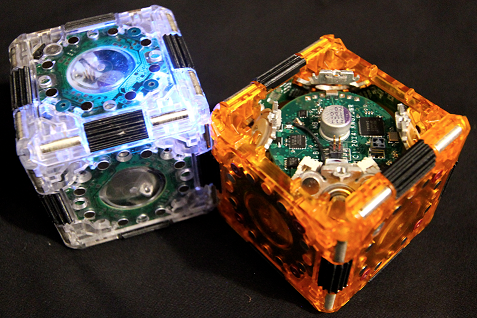
\includegraphics[width=2 in]{figures/cover.png}};
%    		\begin{scope}[x={(image.south east)},y={(image.north west)}]
%		%\node at (0.7,0.5) [align=center, rounded corners, fill=black!10, draw=none,opacity = 0.5]
%			%{$\omega = 0$\\$ V_{x} > 0 $\\ $ V_{y} = 0 $};
%		\draw[line width=1pt,->,red] (0.3,0.5) -- +(0:0.15);
%		\end{scope}
%	\end{tikzpicture}}
%\end{figure}


%%%%%%%%%%%%%%%%%%%%
%%%%%%%%%%%%%%%%%%%%
%%%%%%Old Text%%%%%%
%%%%%%%%%%%%%%%%%%%%%
%%%%%%%%%%%%%%%%%%%%%
%%%%%%%%%%%%%%%%%%%%%

%
%We have constructed four active 3D M-Blocks modules, as well as many
%passive modules. Although the modules share the basic shape and
%magnetic bonding mechanism as the previous one-dimensional system, almost % Mechanism? System? Interface? unsure what word here
%every part has been completely redesigned.  The significant changes  % As or like?
%include the plane changing mechanism, edge gear teeth, and simplified
%secondary magnet arrangement.  The basic parameters of the new module,
%and how they compare with the previous
%version, are shown in Table~\ref{tab:info}.
%
%\begin{table}[h]
%  \caption{Comparison of 3D M-Blocks to first generation M-Blocks. $ \dagger$ Pre-assembled ball bearings and assembled printed circuit boards are counted as single parts.}
%
%  \begin{tabular}{ p{3.4cm}  p{1.9cm}  p{1.9cm} }
%    \hline
%    & M-Blocks & 3D M-Blocks \\
%    \hline
%    Actuation Directions & 1 & 6 \\
%    Mass & 143\,g & 150\,g \\
%    Flywheel Moment of Inertia & 5.7\,E-6\,$\text{kgm}^2$ & 8.4\,E-6\,$\text{kgm}^2$ \\
%    Total Parts $ \dagger$ & 178 & 216 \\
%    Actuated Moving Parts  & 8 & 10 \\
%    Unique Parts & 30 & 46 \\
%    Est. Cost & \$250 & \$130 \\
%    Maximum Torque & 1.6\,Nm & 2.6\,Nm \\
%  \end{tabular}
%
%  \label{tab:info}
%\end{table}
%
%
%The goal of redesigning the M-Blocks was to extend their functionally
%to three dimensions while maintaining robustness and keeping the
%components as simple and mass-producible as possible. In order to
%extend the original M-Blocks concept to three planes, we first
%considered three separate, mutually orthogonal inertial actuators,
%similar to the design for Cubli~\cite{Cubli}.  However it proved
%difficult to fit three separate sets of flywheels, motors, and brakes
%inside the 50\,mm modules while maintaining a torque density sufficient to perform lattice % changed from torque - to moment - of - inertia ratio
%reconfiguration. Despite the added complexity of having to change planes, the advantage in power of a larger single
%flywheel proved to be the better solution.
%
%The redesign has focused on replacing complex actuators with simple
%ones while also attempting to utilize under-actuation where
%possible. For example, the flywheel brake in the 3D M-Blocks is built
%from a coil, two magnets, and a simple linkage.  In contrast, the
%original M-Blocks employed a hobby-style servo motor which was large
%and prone to failure.  Additionally, the orientation of the flywheel
%with respect to the module's frame is now controlled
%by the primary inertial actuator and a locking mechanism instead of an additional motor.
%
%While the 3D M-Blocks have more parts and more mass than their
%predecessors, they are capable of producing a higher maximum torque,
%controlled by more robust and capable electronics, and require less expensive machining.  The modules have proven to be robust,
%undergoing hundreds of reconfiguration movements without degradation,
%and surviving many falls of up to one meter in height.  The remainder
%of this section will describe the mechanical structure of the modules,
%the design of the inertial actuator, the operation of the plane
%changing mechanism, and the details of the electronics which control
%the modules.
%
%%%%%%%%%%%%%%%%%%%%%%%%%%%%%%%%%%%%%%%%%%
%\subsection{Overall Module Design}
%%%%%%%%%%%%%%%%%%%%%%%%%%%%%%%%%%%%%%%%%%
%
%\begin{figure*}[t*]
%
%  \centering
%  \includegraphics[width=6in]{Figures/ExplodedViewWithInsets.png}
%
%  \caption{Each 3D M-Block is built around a six-piece injection
%    molded frame \emph{gray} which supports the central assembly  \emph{lighter
%    gray, split in half} along the frame's longest diagonal axis on
%    two ball bearings  \emph{pink}. The molded frame holds eight magnets colored red and
%blue to represent their magnetic
%polarities. The central assembly holds batteries
%     \emph{yellow} and circuit boards  \emph{green} as well as the flywheel
%     \emph{purple}. The flywheel represents the inertial actuator.  For
%    clarity, the brake assembly is not shown in the exploded-view, it
%    can be seen in the bottom-left inset picture.  The top-right inset
%    picture shows the main PCB.}
%
%  \label{fig:ExplodedView}
%\end{figure*}
%
%
%The 3D M-Blocks consist of four primary mechanical assemblies: a frame
%(1) which holds the central assembly (2) which in turn supports the
%flywheel (3) and the braking mechanism (4).  In addition, the central
%assembly holds the four batteries which power the module and two of
%the printed circuit boards (PCBs) which control it.  The exploded
%view in Figure~\ref{fig:ExplodedView} shows the frame, central
%actuator, flywheel, batteries, and control PCBs.  The two insets in
%Figure~\ref{fig:ExplodedView} show actual photos of the finalized
%central assembly with all components including the braking system.  The braking mechanism is omitted from the exploded view
%because it is shown in better detail in Figure~\ref{fig:Brake}.
%
%At the core of the central assembly is a brushless motor and flywheel
%which, together with the braking mechanism, generate the torques
%required for all module movements and central assembly plane changes.
%The entire central assembly is supported by two ball
%bearings on a diagonal rotational axis which extends through two
%opposite corners of the cubic frame.  As the central actuator rotates
%about this diagonal axis, the flywheel aligns with each of the
%module's coordinate axes.
%
%%%%%%%%%%%%%%%%%%%
%\subsection{Frame}
%\label{sec:Frame}
%%%%%%%%%%%%%%%%%%%
%
%The 50\,mm cubic frame is built from six identical injection-molded
%panels which snap together.  Each panel contains two functional edges which contain two diametrically
%magnetized cylindrical magnets. Furthermore, each panel holds eight smaller
%alignment magnets in the faces.  The details of this magnetic interface configuration are described in
%~\cite{RomanishinRus-IROS13}. This magnetic interface
%allows neighboring modules to pivot about the cylindrical magnets in
%their common edges, and to form face to face bonds.
%
%In the 3D M-Blocks, we have added 15\,mm wide sections of gear teeth
%along each module's edges (shown in black in
%Figure~\ref{fig:ExplodedView}).  These gear teeth prevent slippage as
%two modules pivot relative to one another.  Because the shape of the gear teeth does not
%protrude past the extents of the frame, it does not hinder
%the ability of modules to pivot next to adjacent stationary modules.
%
%Finally, each frame panel holds a face PCB which is used to interface with the
%surrounding environment.
%
%Each of the eight corners of the frame contains an aluminum corner
%brace.  These braces are cut from sheet metal and die-formed so that
%they can be rigidly attached to the three adjacent panels.  In addition to
%adding strength to the frame, two of these corner braces provide rigid
%mounting points for ball bearings which connect the central assembly
%to the frame.  Three additional corner braces contain specialized
%mating holes and magnets which are a part of the plane changing
%mechanism detailed in Section~\ref{sec:PlaneChanging}.
%
%%%%%%%%%%%%%%%%%%%%%%%%%%%%%%%%%%%%%%%%%%%%
%\subsection{Inertial Actuator Design}
%\label{sec:FlywheelAndBraking}
%%%%%%%%%%%%%%%%%%%%%%%%%%%%%%%%%%%%%%%%%%%%
%
%The inertial actuator consists of a flywheel and a self-tightening
%band brake. All of the relevant components which form the actuator are
%illustrated in Figure~\ref{fig:Brake}.
%
%\begin{figure}[htb]
%
%  \centering
%  \includegraphics[width=3.25in]{Figures/brake.png}
%
%  \caption{The inertial actuator operates by quickly decelerating a
%    spinning flywheel \emph{purple} with a neoprene belt \emph{dark gray} that
%    wraps around the flywheel and which is anchored in two
%    arms \emph{yellow}.  The belt is tightened by a linkage
%    \emph{green}, which is supported by ball bearings \emph{pink}, and which acts as a lever to amplify the force felt at the belt (\emph{blue} and \emph{red}  arrows indicated relative motions for both CW and CCW braking actions).  To activate the brake, the coil \emph{orange} briefly generates either a positive or negative magnetic field
%    which exerts a corresponding force on the two magnets \emph{red/blue} which drives the linkage. }
%
%  \label{fig:Brake}
%\end{figure}
%
%The flywheel assembly consists of a thin brass ring with an outer diameter of
%38.0\,mm, inner diameter of 34.0\,mm and a thickness of 10.5\,mm into which the motor's rotor is press-fit.
%This flywheel-rotor assembly is then connected by two bearings, one on
%either side of the stator, to the surrounding frame such that the
%flywheel is completely supported and not cantilevered.  This design
%allows for the motor and flywheel to have a thin profile while
%maintaining a stiff attachment to the frame.  The downside to this
%approach is that the three wires which power the stator must fit
%through the center of the bearings, thereby complicating the assembly
%process.
%
%Once the flywheel is spinning, the 3D M-Blocks use a direct drive
%electromagnetic coil actuator as shown in Figure~\ref{fig:Brake} to activate
%the brake.  We chose this approach for its fast linear response
%(10\,ms), adequate force (3\,N), bidirectionality, low cost, robustness,
%and size.
%
%To exert a torque on the 3D M-Block, the motor first accelerates the flywheel
%to a set speed.  With the motor coasting, the module energizes the
%pancake-shaped coil with 280 turns of \#30 AWG wire to create a magnetic
%field.  This magnetic field exerts forces on the two ring magnets and associated keeper, with one of the magnets attracted towards the center of the coil and the
%other repelled.  The resulting force is transferred and magnified by a ratio of two to one by the
%four-bar linkage to the belt-holder arms. The two belt-holder arms
%are each attached in a one-way lever configuration to their respective
%elements in the four-bar linkage, thus allowing for bi-directional
%motion, despite the physical constraints of the belt-arms. With one
%of the belt holder arms pulling on its end of the belt, the mechanism
%tightens the belt around the flywheel.  The other end of the belt is
%immobilized by a mechanical hard stop.
%
%The current flowing through the coil is always polarized such that the end
%of the belt which is pulled causes the belt to constrict in the same
%direction that the motor is spinning.  As the belt comes into contact
%with the flywheel, the friction between the two surfaces causes the
%belt to self-tighten and completely arrest the flywheel in a matter of
%milliseconds.
%
%This system represents a complete redesign from the previous
%iteration.  The redesign was necessary in order to fit the inertial
%actuator within the spherical constraint imposed on the design.  As
%part of the redesign, the flywheel has been made larger, thicker, and,
%as a result, has a higher moment of inertia which allows
%for larger peak torques to be applied to the module.  The flexible
%neoprene belt used for braking is now 25\% wider and 30\%
%longer, which increases its surface area, resulting in
%increased stopping power with less belt wear.
%
%
%%%%%%%%%%%%%%%%%%%%%%%%%%%%%%%%%%%%%%
%\subsection{Plane Changing Mechanism}
%\label{sec:PlaneChanging}
%%%%%%%%%%%%%%%%%%%%%%%%%%%%%%%%%%%%%%
%
%The central assembly in each 3D M-Block can be thought of as a sphere
%rotating inside of a cube (the frame). In order to fully
%constrain the two assemblies together three points of contact are
%required. Two of these points are formed by ball bearings attaching
%the central assembly to the frame through an axis aligned between two
%opposing corners of the frame (along the longest diagonal).  This
%diagonal axis is offset $35\pi/180$\,radians from that of the
%flywheel's axis of rotation.  This diagonal axis extends through two
%opposite corners of the cubic frame.  As the central actuator rotates
%every $2\pi/3$\,radians about this diagonal axis, the flywheel aligns
%with a different set of the module's faces.  That is, if the flywheel
%is initially aligned with the module's x-axis, rotating the central
%actuator by $2\pi/3$\,radians, in one direction or another, will bring the
%central actuator into alignment with the module's y- or z-axis.
%
%To lock the central assembly into place, a third connection point is
%necessary.  It is formed by a retractable pin which protrudes from the
%central actuator.  When extended, the pin mates with one of three
%matching holes in the frame's corner braces (see
%Figure~\ref{fig:PlaneChanging}).
%
%\begin{figure}[htb]
%
%  \centering
%
%  \begin{subfigure}[b]{.3\linewidth}
%    \includegraphics[width=1in]{Figures/FlywheelX.png}
%    \subcaption{X-axis}
%  \end{subfigure}
%  ~
%  \begin{subfigure}[b]{.3\linewidth}
%    \includegraphics[width=1in]{Figures/FlywheelY.png}
%    \subcaption{Y-axis}
%  \end{subfigure}
%  ~
%  \begin{subfigure}[b]{.3\linewidth}
%    \includegraphics[width=1in]{Figures/FlywheelZ.png}
%    \subcaption{Z-axis}
%  \end{subfigure}
%
%
%%%  \subfloat[X-axis]{\includegraphics[width=1.1in]{Figures/FlywheelX.png}}
%%%  \subfloat[Y-axis]{\includegraphics[width=1.1in]{Figures/FlywheelY.png}}
%%%  \subfloat[Z-axis]{\includegraphics[width=1.1in]{Figures/FlywheelZ.png}}
%
%  \caption{The 3D M-Block changes the alignment of its flywheel by
%    rotating the central assembly along a diagonal axis between two
%    opposite corners of the frame (pointing out of the page).
%    For every $2\pi/3$ radians of rotation along this axis, the
%    flywheel comes into alignment with a new axis of the frame.}
%

%  \label{fig:PlaneChanging}
%\end{figure}
%
%In order to switch planes, the 3D M-Block first spins-up the motor.  Once
%the flywheel has reached a constant speed, the pin is retracted, which allows the central assembly to spin freely on its diagonal
%rotation axis.  A torque is then generated by electronically braking
%the motor.  The component of this torque aligned with the diagonal axis, causes the central assembly to rotate and align with a new plane. Magnets, one embedded in
%the central assembly, and one next to each of the pin alignment holes
%in the frame, provide mechanical detents to assist with fine alignment
%between the central assembly and the frame.  Once the pin is aligned
%with one of the mating holes, it is then extended to lock the central
%assembly into place.
%
%
%%%%%
%%%%%
%%%%%
%%%%%
%%%%%
%
%During experiments with the 3D M-Blocks, we found that the central
%actuator sometimes stopped rotating about the diagonal axis at points
%which left the pin misaligned with the mating holes in the corners of
%the frame.  To combat this, we added additional repulsive magnets near
%one of the bearings which complement the attractive force already
%provided by the magnets near the pin mating holes.  While this change
%greatly reduced the frequency with which the central actuator ends up
%misaligned with the frame, it has also made it difficult for a module
%to change the plane of its central assembly if the module is not
%magnetically attached to a larger lattice.  Without additional mass to
%help immobilize the module, attempting to change the plane of the
%central actuator results in the entire module pivoting about one of
%its edges.  We plan to refine the magnet arrangement in
%order to eliminate this problem in the future.
%
%%%%%
%%%%%
%%%%%
%%%%%
%%%%%
%
%The retractable pin is controlled by a shape memory alloy (SMA) wire
%which contracts when heated.  The particular SMA wire is a 100\,mm long,
%0.25\,mm diameter FLEXINOL, which is contained within a heat-resistant,
%insulating PEEK plastic tube.  This tube insulates the wire from the
%metal structure of the central assembly, and it also allows the wire
%to bend a complete $\pi$\,radians in order to fit the necessary length of
%wire within a constrained area.  One end of the SMA wire is
%electrically connected to a constant current driver on the main
%circuit board.  The other end of the wire is crimped into the
%retractable pin, which touches the central aluminum frame, and
%provides an electrical ground.  A strong (425\,N/m) spring provides the
%necessary restoring force to extend the pin when the SMA is not being
%heated.  As such, the SMA only consumes current when the pin is being
%held in the retracted position.
%
%%%%%%%%%%%%%%%%%%%%%%%%%
%\subsection{Electronics}
%\label{sec:Electronics}
%%%%%%%%%%%%%%%%%%%%%%%%%
%
%The electronics, which control each 3D M-Block, are divided across eight
%different PCBs.  The core functionality comes from a main PCB attached
%to one side of the central actuator.  The main PCB holds a Nordic
%nRF51422 (nRF) microprocessor with an on-chip 2.4\,GHz radio.  The
%radio is capable of supporting both low-energy Bluetooth Smart (which
%we use for centralized control) and the ANT protocol (which we plan to
%use for module-to-module communication).  The nRF is connected via a
%two-wire bus to a 6-axis inertial measurement unit (IMU), the
%MPU-6050, produced by Invensense.  The IMU allows the nRF to determine
%the central actuator's orientation as it rotates.
%
%The central brushless motor control is managed by a dedicated Allegro
%MicroSystems A4960 which frees the main processor for higher-level
%tasks.  While the A4960 handles the low-level motor control,
%closed-loop speed regulation requires supervision from the nRF.  The
%A4960 can apply an electronic braking torque to the motor in order to
%decelerate it more slowly than the mechanical brake.
%
%The main PCB also includes circuitry to control the shape memory alloy
%(SMA) wire, which retracts the pin. The pin locks the central actuator
%into alignment with each of the 3D M-Block's coordinate planes.  The
%circuitry is based on a high-current LED driver and a low-side current
%sense amplifier. It is capable of driving a maximum of 1.5\,A through
%the SMA wire, but due to the relatively slow thermal response of the
%SMA, we modulate the current on and off to achieve sufficient force
%without overheating the SMA wire.  When retracting the pin, we apply
%an average of 1.2\,A for 2\,s, but once retracted, we have found
%that we only need to apply an average of 700\,mA to hold the pin
%stationary.
%
%Finally, the main PCB includes charging and balancing circuitry for
%the four 125\,mAh lithium-polymer batteries which power each 3D M-Block.
%The batteries are connected in series in order to supply sufficient
%voltage to drive the motor at speeds over 20,000\,RPM.  Charging is
%enabled by connecting the M-Block to a 5\,V, 500\,mA source (e.g. a USB
%port).  An on-board, current-limited boost converter controls the
%voltage and current delivered to the batteries.  If the nRF detects
%that one battery's voltage is exceeding that of the others, it
%switches in an additional resistive load across that battery thereby
%reducing its charge rate and keeping all batteries balanced.
%
%A battery protection IC independently monitors each battery's voltage
%and current drain and disconnects all batteries if it detects a fault
%condition.  The main PCB also includes additional reverse-voltage,
%over-current, over-temperature, and electrostatic discharge protection
%devices in recognition of the fact that the M-Blocks must remain
%robust when being deployed outside of the laboratory environment.
%
%To complement the main PCB, there is a daughter PCB attached to the
%opposite side of the central actuator.  The two PCBs communicate
%over the aforementioned two-wire bus with the nRF acting as the bus
%master.  In addition to providing the connection point for two of the
%four batteries, the daughter PCB holds the circuitry which drives
%current through the mechanical braking coil.  The braking circuitry is
%controlled by an STMicroelectronics STM32F051 microprocessor which is
%a slave on the two-wire bus.  The braking circuitry is based on an
%op-amp which linearizes a current-controlling PMOS device in order to
%provide continuous current control from 0 to 4\,A.
%
%The main and daughter PCBs are complemented by six face PCBs, which are
%embedded into each face of the frame.  At the moment, the face
%PCBs provide convenient electrical contacts through which to
%charge the batteries.  In the near future, Atmel ATtiny1634 processors
%on each of the face PCBs will enable infrared communication between
%neighboring M-Blocks.  There is also a footprint for a second IMU on
%the face PCBs so that the central actuator will be able to determine
%its position relative to that of the surrounding frame.  Like the
%processor on the daughter PCB, the Atmel processors will be slaves on
%the same two-wire communication bus.
%
%The face PCBs are electrically connected to the central assembly by
%custom slip rings formed by the bearings that support the central
%assembly.  One bearing is in direct electrical contact with the
%central assembly and provides a ground connection, while the other is isolated and carries one of the bus lines
%to the face PCBs.  We employ a brass pin, which
%passes through the center of the each bearing to carry 3.3\,V to the
%face PCBs.  The pin contacts a leaf spring soldered to one of the
%face PCBs.  Experiments have shown that the
%bearings present several Ohms of resistance. However, the face PCBs do not
%require high currents, so this is not problematic.
%When power is flowing into the central assembly during the charging process, the voltage drop
%across the bearings can be compensated for by an increase of the external
%charging voltage.


\section{Behaviors}
\label{sec:Behaviors}

The three behaviors described in Section~\ref{sec:Introduction} are described in more detail in this section. 

%%%%%%%%%%%%%%%%%%%%%%%%%%%%%%%%%%%%%%%%%%%%%%%%%%%%%%%%%%%%%%%%%%%%%%%%%%%%%%%%%%%%%%%%%%%%%%%%%%%%%%%%%%%%%%%%%%%%%%%%%%%%%%%%%%%%%%%%%%%%%%%
%%%%%%%%%%%%%%%%%%%%%%%%%%%%%%%%%%%%%%%%%%%%%%%%%%%%%%%%%%%%%%%%%%%%%%%%%%%%%%%%%%%%%%%%%%%%%%%%%%%%%%%%%%%%%%%%%%%%%%%%%%%%%%%%%%%%%%%%%%%%%%%
\subsection{Arrow Following Behavior}
\label{sec:algArrow}
%%%%%%%%%%%%%%%%%%%%%%%%%%%%%%%%%%%%%%%%%%%%%%%%%%%%%%%%%%%%%%%%%%%%%%%%%%%%%%%%%%%%%%%%%%%%%%%%%%%%%%%%%%%%%%%%%%%%%%%%%%%%%%%%%%%%%%%%%%%%%%%
%%%%%%%%%%%%%%%%%%%%%%%%%%%%%%%%%%%%%%%%%%%%%%%%%%%%%%%%%%%%%%%%%%%%%%%%%%%%%%%%%%%%%%%%%%%%%%%%%%%%%%%%%%%%%%%%%%%%%%%%%%%%%%%%%%%%%%%%%%%%%%%
This algorithm attempts to drive a cube in the direction of the embedded direction defined by the \tagName on its neighbor cubes. This 
	
\begin{algorithm}[ht] 
	%\hrulefill
	\caption{Arrow Following Algorithm}
	\label{algorithmArrow}
	\SetAlgoLined
	\KwData{M-Blocks 3D}
	initialization\;
	\While{Connected to Valid module}
	{
		determine arrow direction\;
		\eIf{Flywheel plane is aligned with arrow}
		{
			Move in direction of arrow\;
		}
		{
			 Attempt to align flywheel with correct plane\;
		}
	}
	\caption{This algorithm attempts to drive a cube in the direction of the embedded direction defined by the \tagName on its neighbor cubes}

\end{algorithm}

\subsection{3D Line Formation Behavior}
\label{ssec:algline}
The goal of this experiment is to reconfigure an arbitrary 3D structure into a line. There are several approaches that could be applied to this, from implementing the full 3D algorithm described in ~\cite{sung2015reconfiguration}, to more simple approaches. These simple approaches could even be mostly distributed, for example, each module could check to see if it is part of the line (By asking through WIFI, or checking some local indicator, e.g. if the module it is attached to has its LED's turned on), and if not pick a direction and move that way. If it gets stuck, it will try to detach from the structure and try to randomly attach back and try again.

\begin{algorithm}[ht] 
	%\hrulefill
	\caption{Line formation Algorithm}
	\label{algorithmLine}
	\SetAlgoLined
	\KwData{M-Blocks 3D}
	initialization\;
	\While{Not part of line}
	{
		Update sensors and state\;
		\eIf{Neighbors = 1 and movement possible}
		{
			Move in a consistant direction \;
		}
		{
			Attempt to align flywheel with correct plane\;
		}
	}
	\caption{This algorithm attempts to turn an arbitrary 3D shape configuration of modules into a line.}
\end{algorithm}


%%%%%%%%%%%%%%%%%%%%%%%%%%%%%%%%%%%%%%%%%%%%%%%%%%%%%%%%%%%%%%%%%%%%%%%%%%%%%%%%%%%%%%%%%%%%%%%%%%%%%%%%%%%%%%%%%%%%%%%%%%%%%%%%%%%%%%%%%%%%%%%
%%%%%%%%%%%%%%%%%%%%%%%%%%%%%%%%%%%%%%%%%%%%%%%%%%%%%%%%%%%%%%%%%%%%%%%%%%%%%%%%%%%%%%%%%%%%%%%%%%%%%%%%%%%%%%%%%%%%%%%%%%%%%%%%%%%%%%%%%%%%%%%
\subsection{Light Gradient based aggregation Behavior}
\label{sec:algLight}
%%%%%%%%%%%%%%%%%%%%%%%%%%%%%%%%%%%%%%%%%%%%%%%%%%%%%%%%%%%%%%%%%%%%%%%%%%%%%%%%%%%%%%%%%%%%%%%%%%%%%%%%%%%%%%%%%%%%%%%%%%%%%%%%%%%%%%%%%%%%%%%
%%%%%%%%%%%%%%%%%%%%%%%%%%%%%%%%%%%%%%%%%%%%%%%%%%%%%%%%%%%%%%%%%%%%%%%%%%%%%%%%%%%%%%%%%%%%%%%%%%%%%%%%%%%%%%%%%%%%%%%%%%%%%%%%%%%%%%%%%%%%%%%
The goal of this experiment is to aggregate a group of modules nearby a light source to form one assembly. Placing the light source in a corner, and providing a \emph{seed} module can help to simplify aggregation, since the modules would know when to stop (When they see the seed module, or connect to a different module that has previously seen the seed module). One possible biological inspiration for this experiment is to imagine that the modules are cells of a plant, and the algorithm is to grow a structure towards the light source as a plant. As far as I know this work would be the first to accomplish this task in 3 dimensions using modular robots.
%
%\begin{figure}[h]  
%	\centering
%	
%	\begin{subfigure}[b]{0.3\linewidth}
%		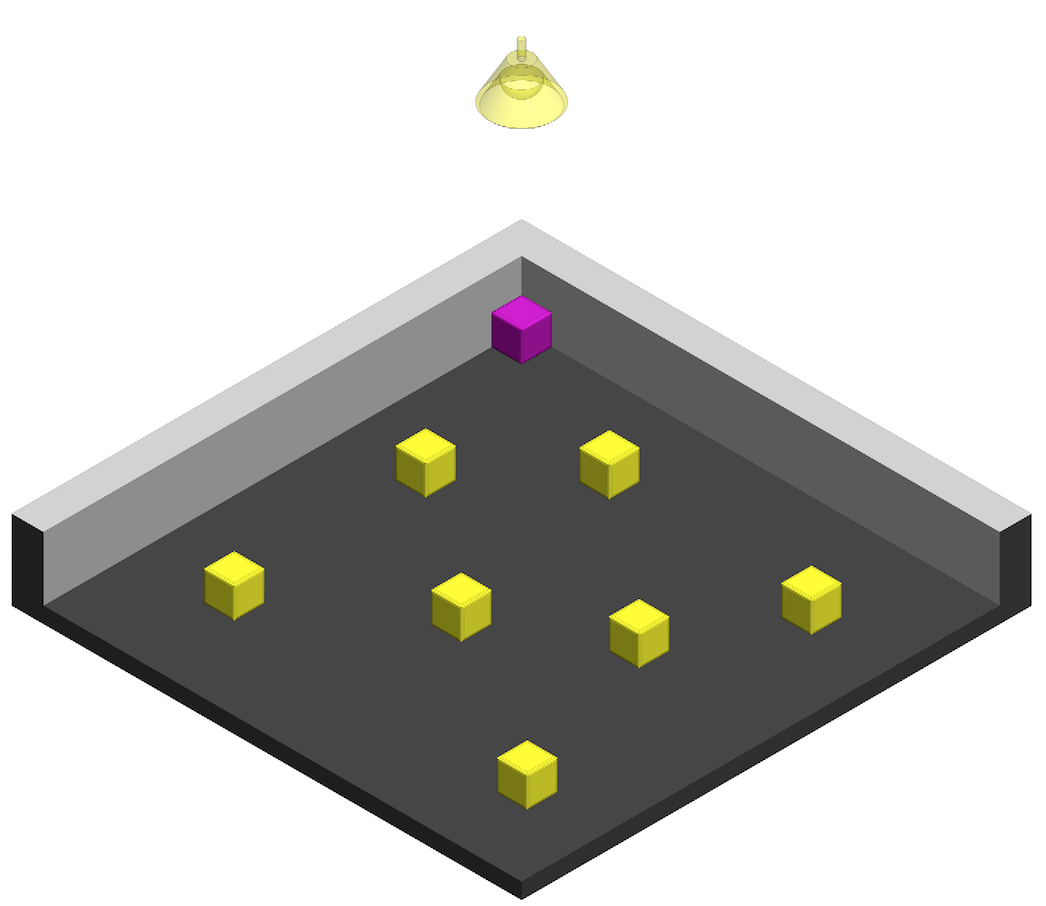
\includegraphics[width=0.9\linewidth]{figures/light_1.png}
%		\subcaption{} 
%	\end{subfigure}
%	\begin{subfigure}[b]{0.3\linewidth}
%		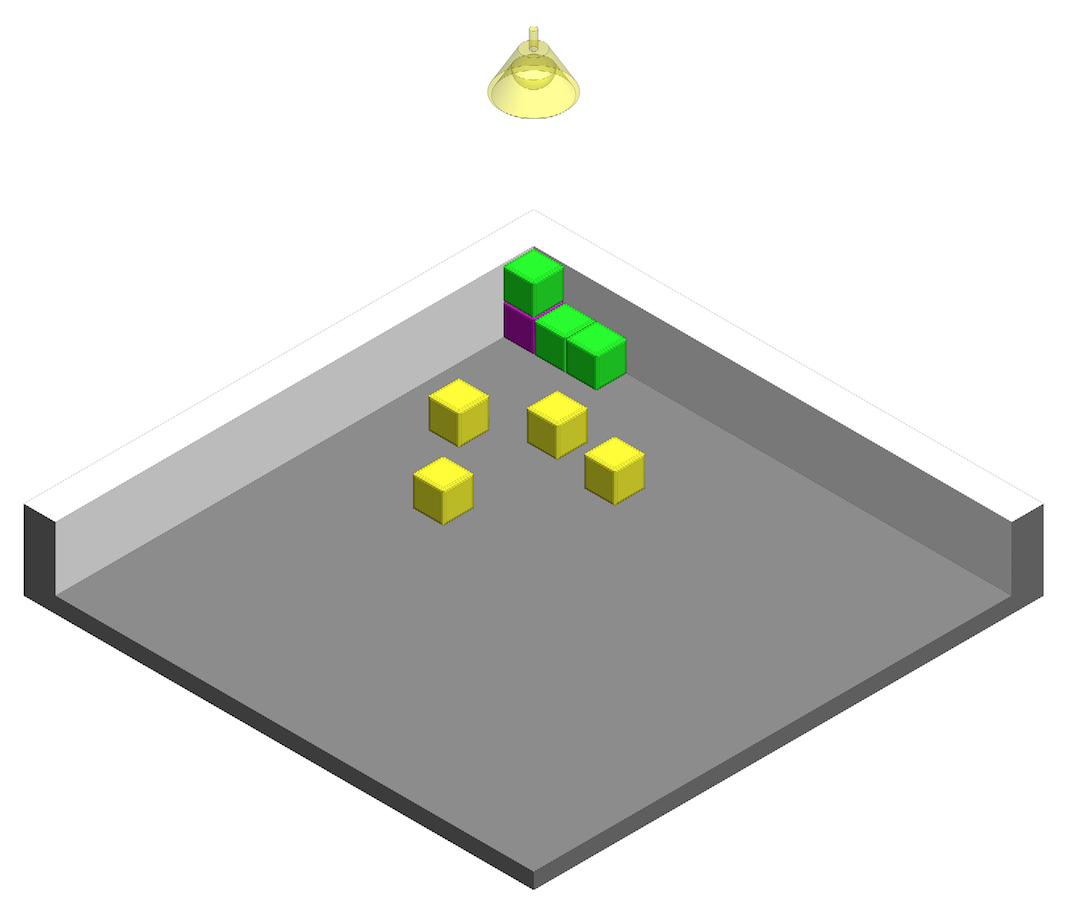
\includegraphics[width=0.9\linewidth]{figures/light_2.png}
%		\subcaption{} 
%	\end{subfigure}
%	\begin{subfigure}[b]{0.3\linewidth}
%		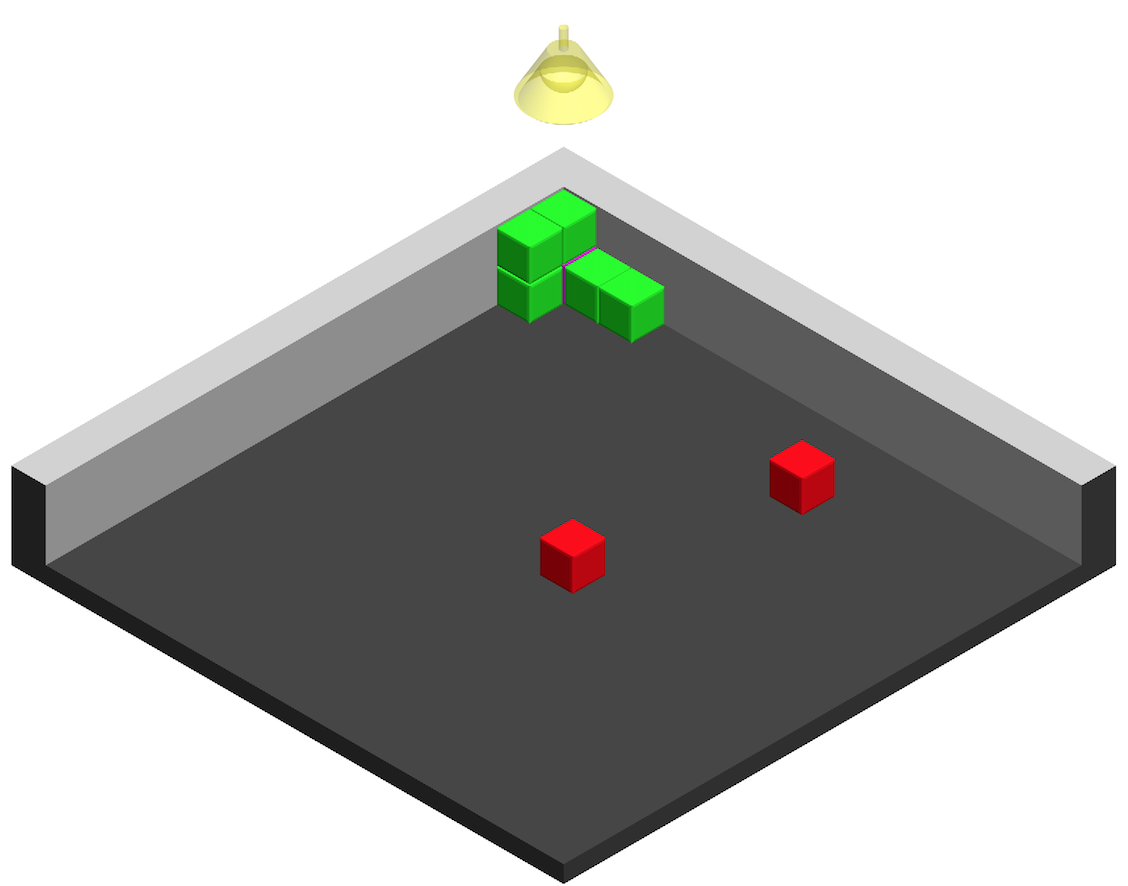
\includegraphics[width=0.9\linewidth]{figures/light_3.png}
%		\subcaption{} 
%	\end{subfigure}
%	
%	\caption{Three frames from an a illustration of the light-seeking experiment. One seed cube \emph{purple} is placed near the light, and the cubes in \emph{yellow} attempt to move towards the light. In the final frame, the modules which are in \emph{green} successfully reached the goal, while modules that are \emph{red} did not manage to join the target structure.}
%	
%	\label{fig:light}
%\end{figure}

\begin{algorithm}[htbp] 
	%\hrulefill
	\caption{Light guided aggregation Algorithm}
	\label{algorithmAggregate}
	\SetAlgoLined
%	\Kw{M-Blocks 3D}
%	initialization\;
	\While{Not connected to Goal Configuration}
	{
		Update State read sensors\;
		\uIf{Numer of Neighbors  = 0}
		{
			Roll in direction of the brightest face that isn't on top\;
		}
		\uElseIf{Neighbors = 1, but not at Goal}
		{
			Run algorithm to attempt to move towards light as a group\;
		}
		\uElseIf{Neighbors = 2, but not at Goal}
		{
			Disconnect from structure
		}
	}
	\caption{This algorithm attempts to drive a group of modules to form a single aggregated group based on following a light gradient.}
	
\end{algorithm}


%begin{figure}[h]  
%\centering
%
%\begin{subfigure}[b]{0.3\linewidth}
%	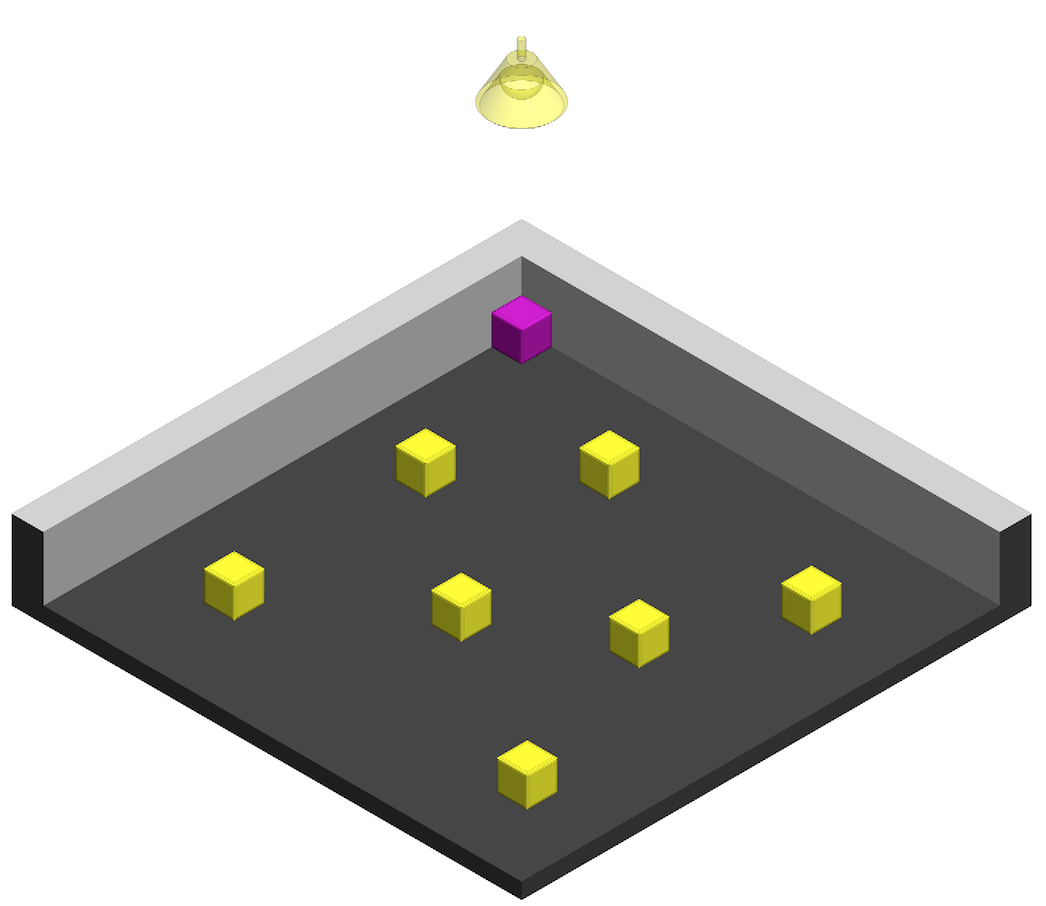
\includegraphics[width=0.9\linewidth]{figures/light_1.png}
%	\subcaption{} 
%\end{subfigure}
%\begin{subfigure}[b]{0.3\linewidth}
%	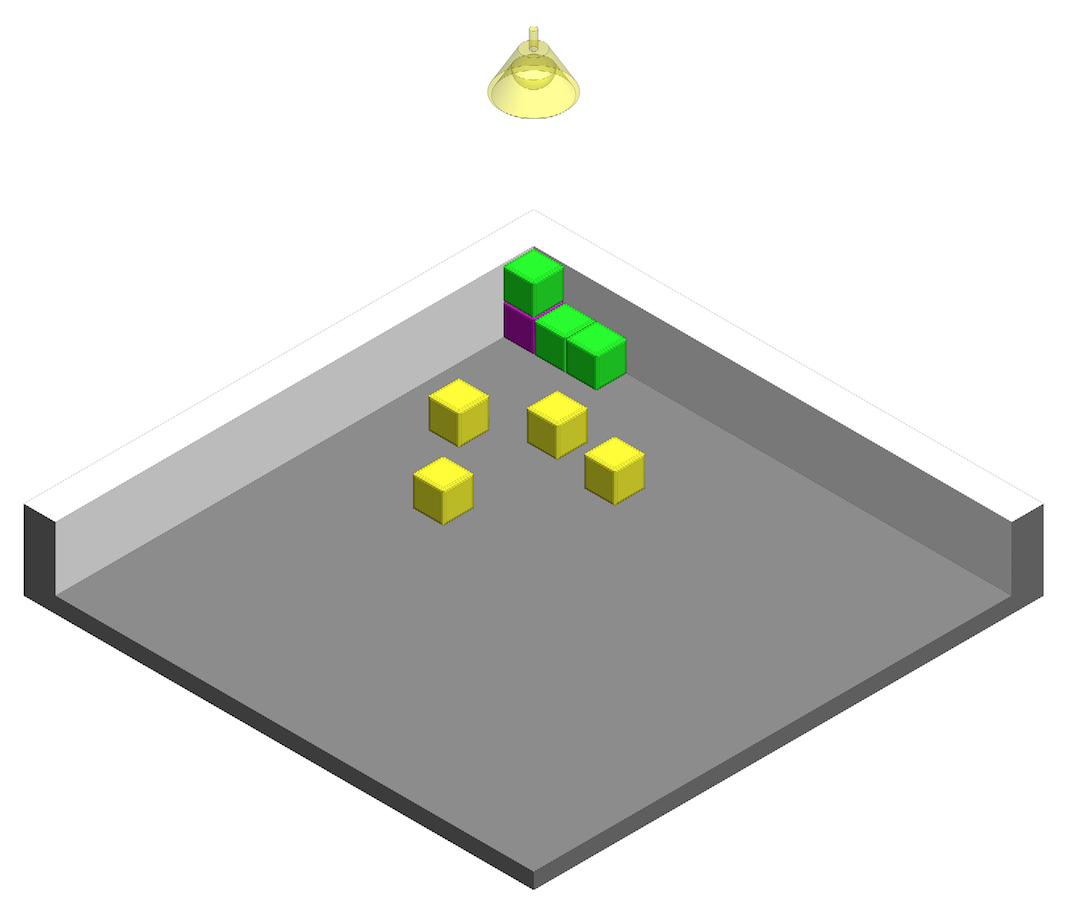
\includegraphics[width=0.9\linewidth]{figures/light_2.png}
%	\subcaption{} 
%\end{subfigure}
%\begin{subfigure}[b]{0.3\linewidth}
%	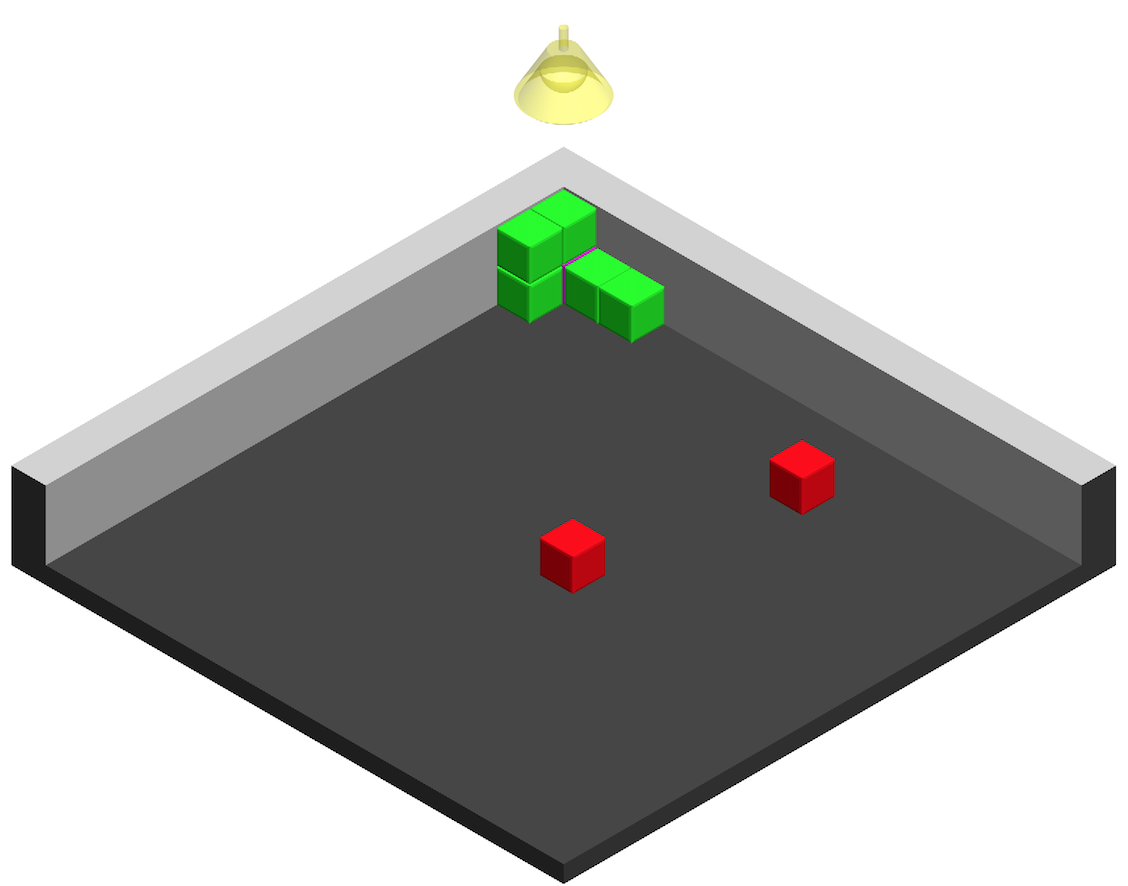
\includegraphics[width=0.9\linewidth]{figures/light_3.png}
%	\subcaption{} 
%\end{subfigure}
%
%\caption{Three frames from an a illustration of the light-seeking experiment. One seed cube \emph{purple} is placed near the light, and the cubes in \emph{yellow} attempt to move towards the light. In the final frame, the modules which are in \emph{green} successfully reached the goal, while modules that are \emph{red} did not manage to join the target structure.}
%
%\label{fig:light}
%\end{figure}

%
%\begin{figure}[h]  
%	\centering
%	\begin{subfigure}[b]{0.3\linewidth}
%		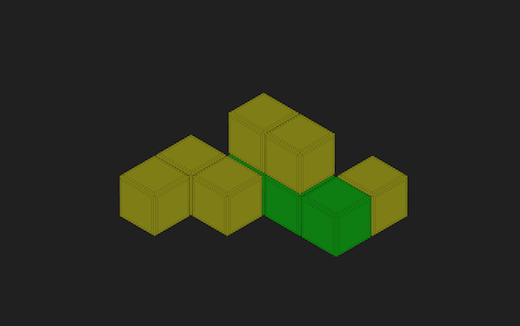
\includegraphics[width=0.9\linewidth]{figures/line_1.png}
%		\subcaption{} 
%	\end{subfigure}
%	\begin{subfigure}[b]{0.3\linewidth}
%		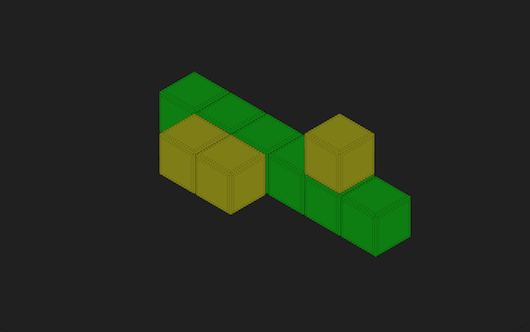
\includegraphics[width=0.9\linewidth]{figures/line_2.png}
%		\subcaption{} 
%	\end{subfigure}
%	\begin{subfigure}[b]{0.3\linewidth}
%		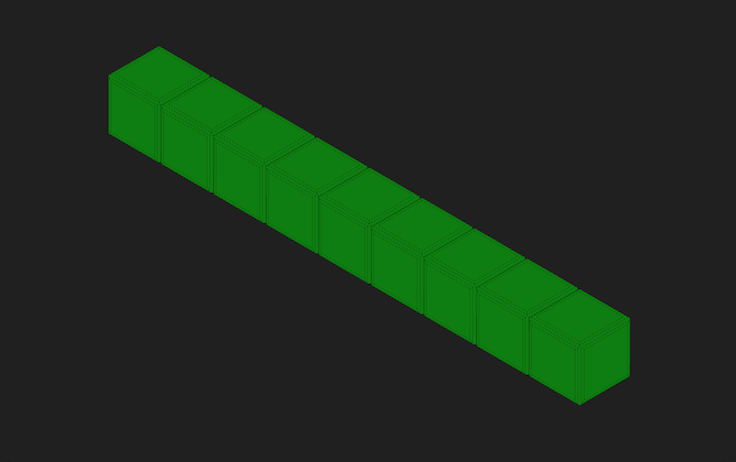
\includegraphics[width=0.9\linewidth]{figures/line_3.png}
%		\subcaption{} 
%	\end{subfigure}
%	
%	\caption{This experiment shows a random 3D configuration of M-Blocks reconfiguring into a line.}
%	
%	\label{fig:line}
%\end{figure}

\section{Experiments}
\label{sec:Experiments}

These algorithms and the resulting behaviors were implemented on a set of twelve 3D M-Block modules. The control system which is running the experiments is described in Figure~\ref{fig:electroncsChart}.

\begin{figure}[ht]

	%% Figure of electronics Diagram
\tikzset{box/.style={draw, rectangle, rounded corners, thick, node distance=7em, text width=6em, text centered, minimum height=3.5em}}
\tikzset{container/.style={draw, rectangle, rounded corners, dashed, inner sep=1em}}
\tikzset{line/.style={draw, thick, -latex'}}

\begin{tikzpicture}[auto]
	\node[anchor=south west,inner sep=0, minimum width = \linewidth, minimum height = 8.5cm] (emptyBox) at (0,0) {};
	\begin{scope}[x={(emptyBox.south east)},y={(emptyBox.north west)}]
	\tikzset{>=latex}
		\coordinate (leftCenter) at (0.12, 0.75);
		\coordinate (rightCenter) at (0.6, 0.85);
		\coordinate (routePt) at (0.50, 0.75);
		
		% Main Board
		\node [box] (mainBoard) at (leftCenter) {High Level Control Board (ESP8266)};
		
		% Kyles Boards...
	%	\node [box] at ([shift = ({225:3.5 cm})] mainBoard) (kb) {Motor and Power Board (nRF51422)};
	%	\node [box, right = 1.5cm of kb] (db)  {Actuator Control Board};
		
		% Face Boards
		\node [box] (f0) at (rightCenter) {Face 0 PCB  (IO~Expander)};
		\node [box, below = 0.25cm of f0] (f1) {Face 1 PCB   (IO~Expander)};
		\node [below = 0.75cm of f1] (f2) {...};
		\node [box, below = 0.75cm of f2] (f5) {Face 5 PCB   (IO~Expander)};
		
		%% I2C Connections
		\path [line, <->, orange, ultra thick] (mainBoard) -- (routePt)-- (f0);
		\path [line, <->, orange, ultra thick] (mainBoard) -- (routePt)-- (f1);
		\path [line, <->, orange, ultra thick] (mainBoard) -- (routePt)-- (f5);
		
	%	\path [line, <->, orange, ultra thick] (kb) -- (db);
		
		%% Serial Connections
		
	%	\path [line, <->, blue, ultra thick] (kb) -- (mainBoard);

		%% Inputs
		\node [align = center] (input1) at (0.91, 0.45) {Environmental \\ and \\ Neighbor \\ sensing};
	%	\node [align = left] (input2) at (0.16, 0.96) {wifi commands};

	%	\node [align = left] (input3) at (0.25, 0.24) {Motor \\ Batteries \\ SMA wire};
	%	\node [align = left] (input4) at (0.4, 0.24) {Brake \\ Em coil};
		
%		\draw [dashed,  <->] (kb.south) to [out = 270, in = 180] (input3.west);
%		\draw [dashed,  <->] (input2.south) to [out = 270, in = 235] (mainBoard.west);
%		\draw [dashed,  <->] (input4.east) to [out = 0, in = 325] (db.east);
		
		\draw [dashed,  ->] (input1.north) to [out = 90, in = 0] (f0.east);
		\draw [dashed,  ->] (input1.north) to [out = 90, in = 0] (f1.east);
		\draw [dashed,  ->] (input1.south) to [out = 270, in = 0] (f5.east);
		
		% Dashed Boxes
	%	\node[container, fit = (mainBoard) (kb) (db) (input4) (input3)] (core) {};
	%	\node at (core.south) [below, node distance = 0 and 0] {\textbf{Core}};

		\node[container, fit = (f0) (f5)] (frame) {};
		\node at (frame.south) [below, node distance = 0 and 0] {\textbf{Frame}};

%    	\node [box] (planning) {Planning};
%   	 	\node [box, below of=planning, maroon, inner sep = 0pt] (resources) {Resources};
%   	 	\node [box, below of=resources] (sensors) {Sensors};
%    	\node [box, below of=sensors] (processing) {Processing};
%    	\node [box, below of=sensors] (processing) {Processing};
%    	\node [box, below of=sensors] (processing) {Processing};
%
%    	\coordinate (middle) at ($(resources.west)!0.5!(sensors.west)$);
%    	\node [box, above of=middle, node distance=4 cm] (archive) {Archive};
%    	\node [box, below of=archive, node distance=4 cm] (reporting) {Reporting};
%
%    	\node[container, fit=(resources) (sensors)] (or) {};
%    	\node at (or.north west) [above right,node distance=0 and 0] {OR};
%
%	    \node[container, fit=(archive) (reporting)] (his) {};
%    	\node at (his.north west) [above right,node distance=0 and 0] {HIS};
%
%    	\path [line, line width = 0.5mm, red] (planning) -- (resources);
%    	\path [line] (resources) -- (sensors);
%    	\path [line] (sensors) -- (processing);
%
%    	\path [line] (archive) |- (planning);
%    	\path [line] (archive) |- (processing);
%    	\path [line] (processing)--($(processing.south)-(0,0.5)$) -| (reporting);
%
%    	\draw [line] ($(processing.south)-(0,0.5)$) -- ++(4,0) node(lowerright){} |- (planning.east);
%    	\draw [line] (lowerright |- or.east) -- (or.east -| resources.south east);
%
%    	\draw[line] (archive.170)--(reporting.10);
%    	\draw[line] (reporting.350)--(archive.190);
    \end{scope}
\end{tikzpicture}


%
%
%	\begin{tikzpicture}
%	\node[anchor=south west,inner sep=0] (image) at (0,0) {\includegraphics[width=0.9\textwidth]{some_image.jpg}};
%	\begin{scope}[x={(image.south east)},y={(image.north west)}]
%
%	\end{scope}
%	\end{tikzpicture}
%\end{document}
	
\caption{This figure illustrates the various avenues of information exchange between the different elements of the experimental setup. The \emph{orange} arrows represent bi-directional WiFi messages sent between the immobile \emph{Server Module} and the active modules, with the dashed line showing a potentially faulty connection. The \emph{blue} arrows show the simple light-based messages which active modules are able to send to neighbors that they are directly connected to. The \emph{purple} arrows represent the reading of \tagNamePlural~ between an active module and a valid and adjacently connected \tagName. Note that \tagNamePlural can be read from both passive modules, and from passive or even unresponsive modules.}
	
	\label{fig:electroncsChart}
\end{figure}

\begin{table}[h]
	\caption{Experimental results for informal experiments testing the three behaviors. See the supplementary materials for the original videos of the experiments.}
	
	\begin{tabular}{ p{2.4cm}  p{1.8cm}  p{1.4cm} p{1.3cm} }
		\hline
								& Path Following& Aggregation 	& Line		\\
		\hline
		Experiments				&  15 			& 3				& 11 		\\
		Successful moves		&  104			& -				& 81			\\
		Failed moves			&  15			& -				& 10			\\
		Failed tag Readings		&  3			& -				& 4			\\
		Reach Goal				&  16/23		& 15 / 30		& 64/84		\\

		
		
		
		
		
		
	\end{tabular}
	
	\label{tab:info}
\end{table}

%%%%%%%%%%%%%%%%%%%%%%%%%%%%%%%%%%%%%%%%%%%%%%%%%%%%%%%%%%%%%%%%%%%%%%%%%%%%%%%%%%%%%%%%%%%%%%%%%%%%%%%%%%%%%%%%%%%%%%%%%%%%%%%%%%%%%%%%%%%%%%%
%%%%%%%%%%%%%%%%%%%%%%%%%%%%%%%%%%%%%%%%%%%%%%%%%%%%%%%%%%%%%%%%%%%%%%%%%%%%%%%%%%%%%%%%%%%%%%%%%%%%%%%%%%%%%%%%%%%%%%%%%%%%%%%%%%%%%%%%%%%%%%%
\subsection{Arrow Following experiments}
\label{sec:mblocksExperimentsArrow}
%%%%%%%%%%%%%%%%%%%%%%%%%%%%%%%%%%%%%%%%%%%%%%%%%%%%%%%%%%%%%%%%%%%%%%%%%%%%%%%%%%%%%%%%%%%%%%%%%%%%%%%%%%%%%%%%%%%%%%%%%%%%%%%%%%%%%%%%%%%%%%%
%%%%%%%%%%%%%%%%%%%%%%%%%%%%%%%%%%%%%%%%%%%%%%%%%%%%%%%%%%%%%%%%%%%%%%%%%%%%%%%%%%%%%%%%%%%%%%%%%%%%%
%%%%%%%%%%%%%%%%%%%%%%%%%%%%%%%%%%%%%%%%%%
This experiment tested the ability of the Modules to identify and follow the "arrows" embedded in in a set of passive and temporarily disabled active modules. The experiment consisted of a single module following the algorithm presented in Section~\ref{sec:algArrow}.

\begin{figure}[h]  
	\centering
	\begin{subfigure}[b]{0.30\linewidth}
		\begin{tikzpicture}[]	
		\node[opacity = 0.95] at (0,0) {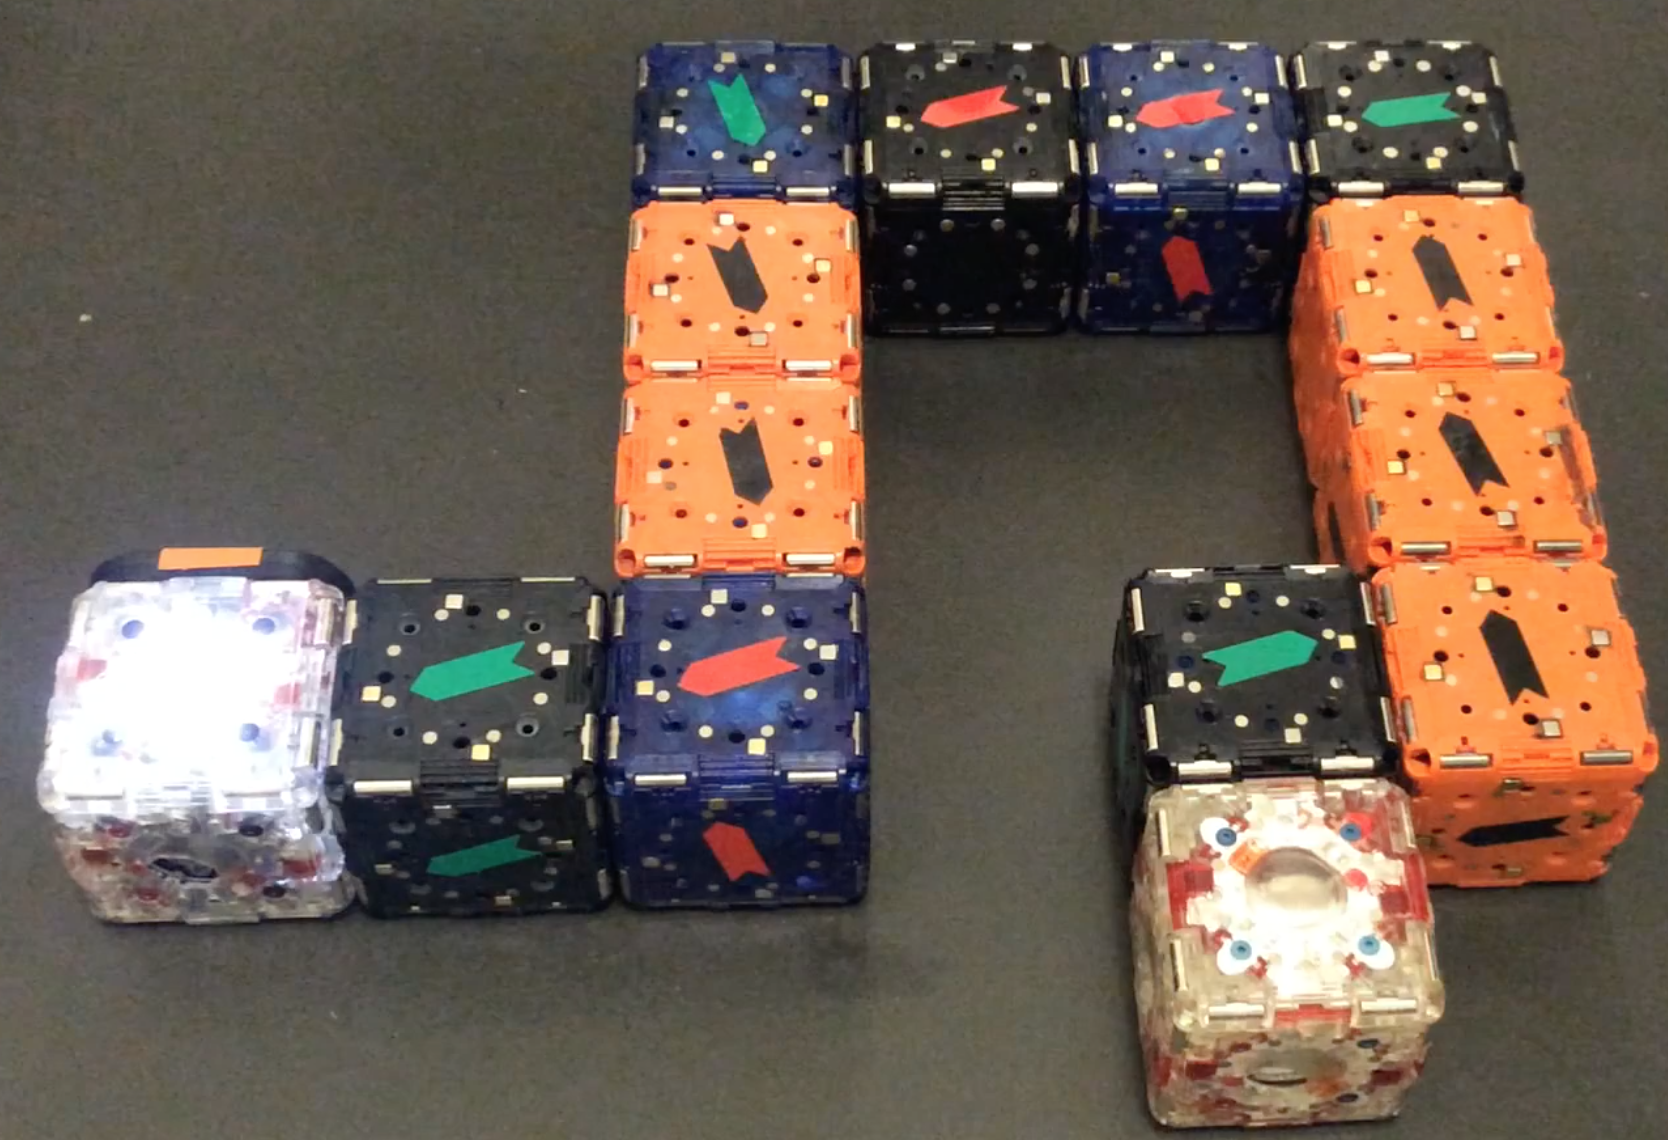
\includegraphics[width=0.97\linewidth]{figures/arrows_0.png}};
		\node[opacity = 0.5, fill = white, rounded corners] at (-0.25,-0.5) {t = 0 s};
		\end{tikzpicture}
	\end{subfigure}
	\begin{subfigure}[b]{0.30\linewidth}
		\begin{tikzpicture}[]	
		\node[opacity = 0.95] at (0,0) {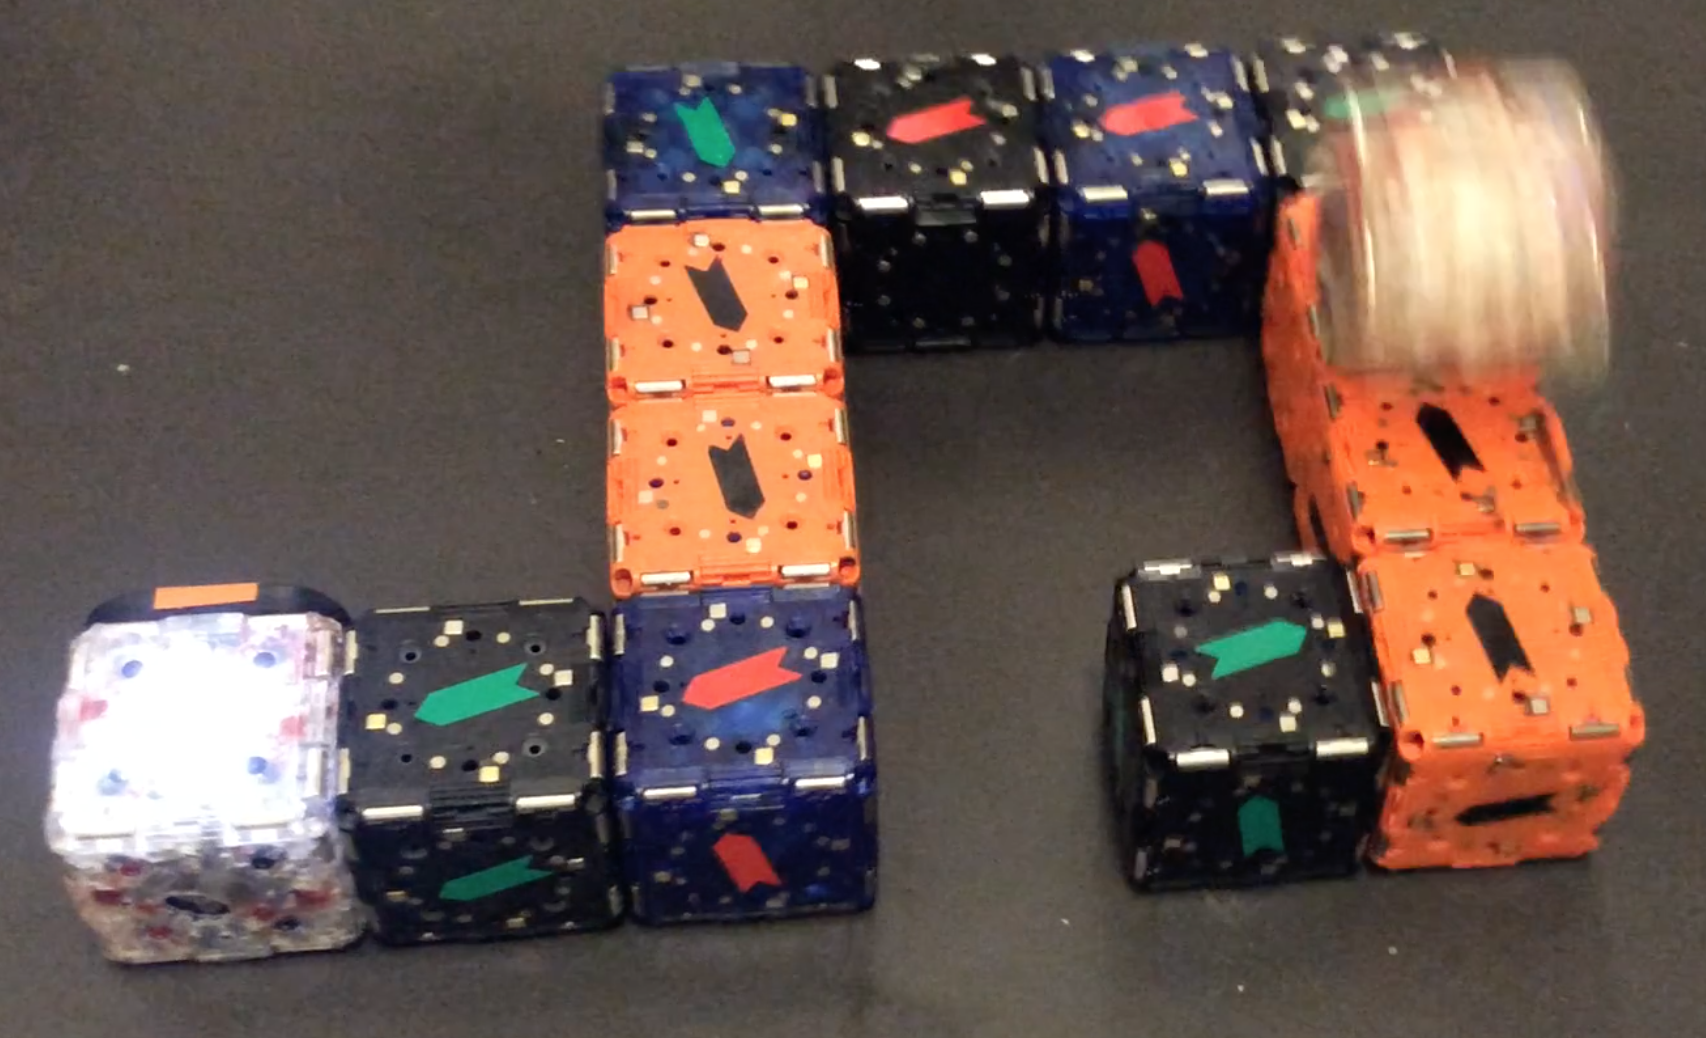
\includegraphics[width=0.97\linewidth]{figures/arrows_227.png}};
		\node[opacity = 0.5, fill = white, rounded corners] at (-0.25,-0.5) {t = 227 s};
		\end{tikzpicture}
	\end{subfigure}
	\begin{subfigure}[b]{0.30\linewidth}
		\begin{tikzpicture}[]	
		\node[opacity = 0.95] at (0,0) {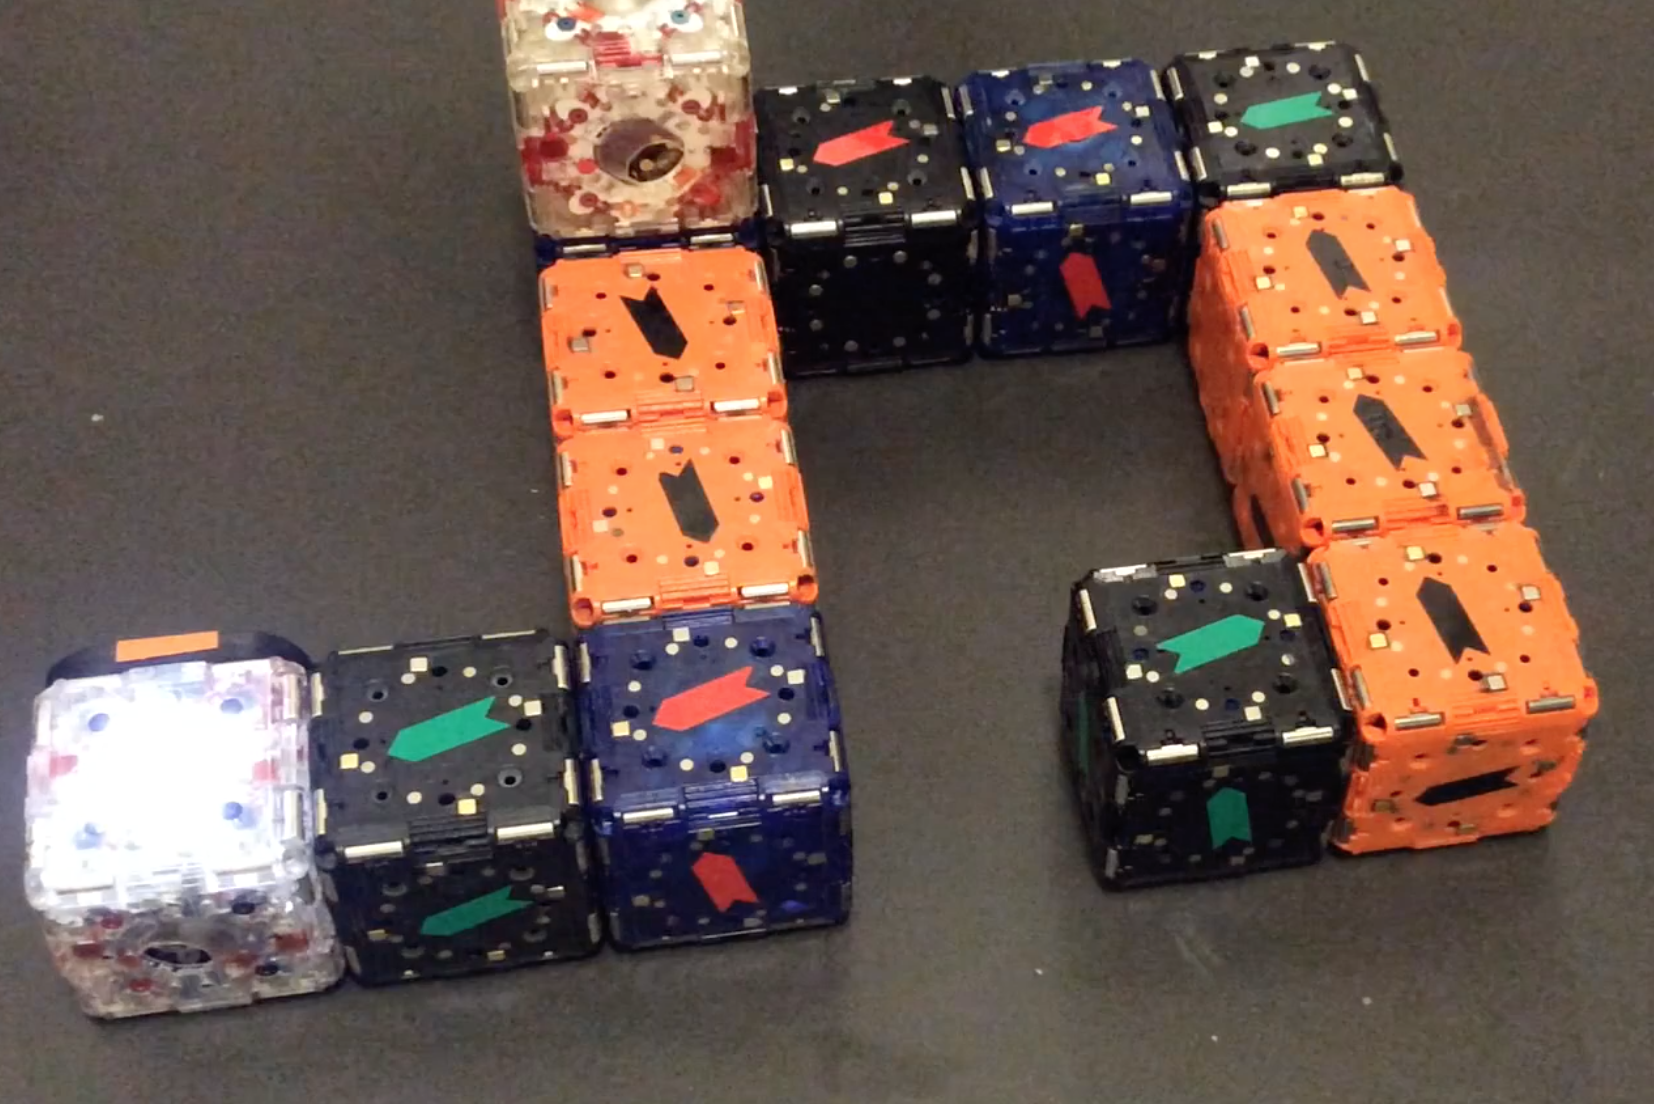
\includegraphics[width=0.97\linewidth]{figures/arrows_421.png}};
		\node[opacity = 0.5, fill = white, rounded corners] at (-0.25,-0.5) {t = 421 s};
		\end{tikzpicture}
	\end{subfigure}

	\begin{subfigure}[b]{0.30\linewidth}
		\begin{tikzpicture}[]	
		\node[opacity = 0.95] at (0,0) {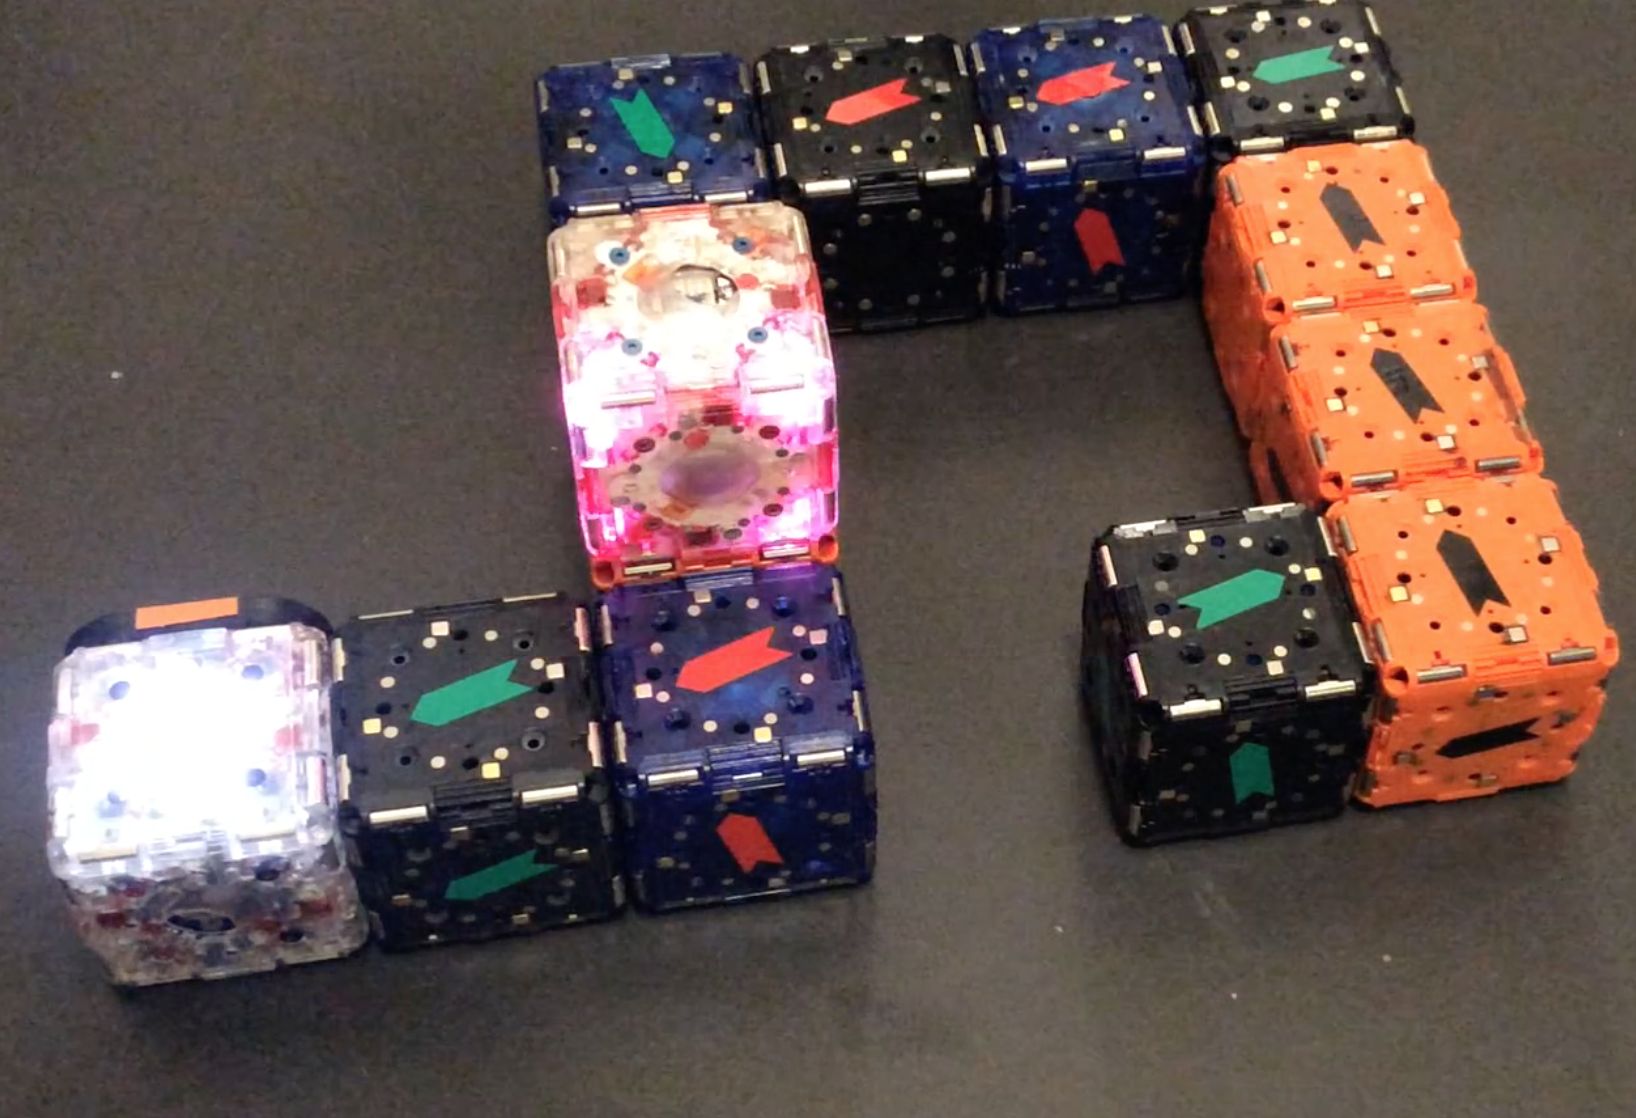
\includegraphics[width=0.97\linewidth]{figures/arrows_660.png}};
		\node[opacity = 0.5, fill = white, rounded corners] at (-0.25,-0.5) {t = 660 s};
		\end{tikzpicture}
	\end{subfigure}
	\begin{subfigure}[b]{0.30\linewidth}
		\begin{tikzpicture}[]	
		\node[opacity = 0.95] at (0,0) {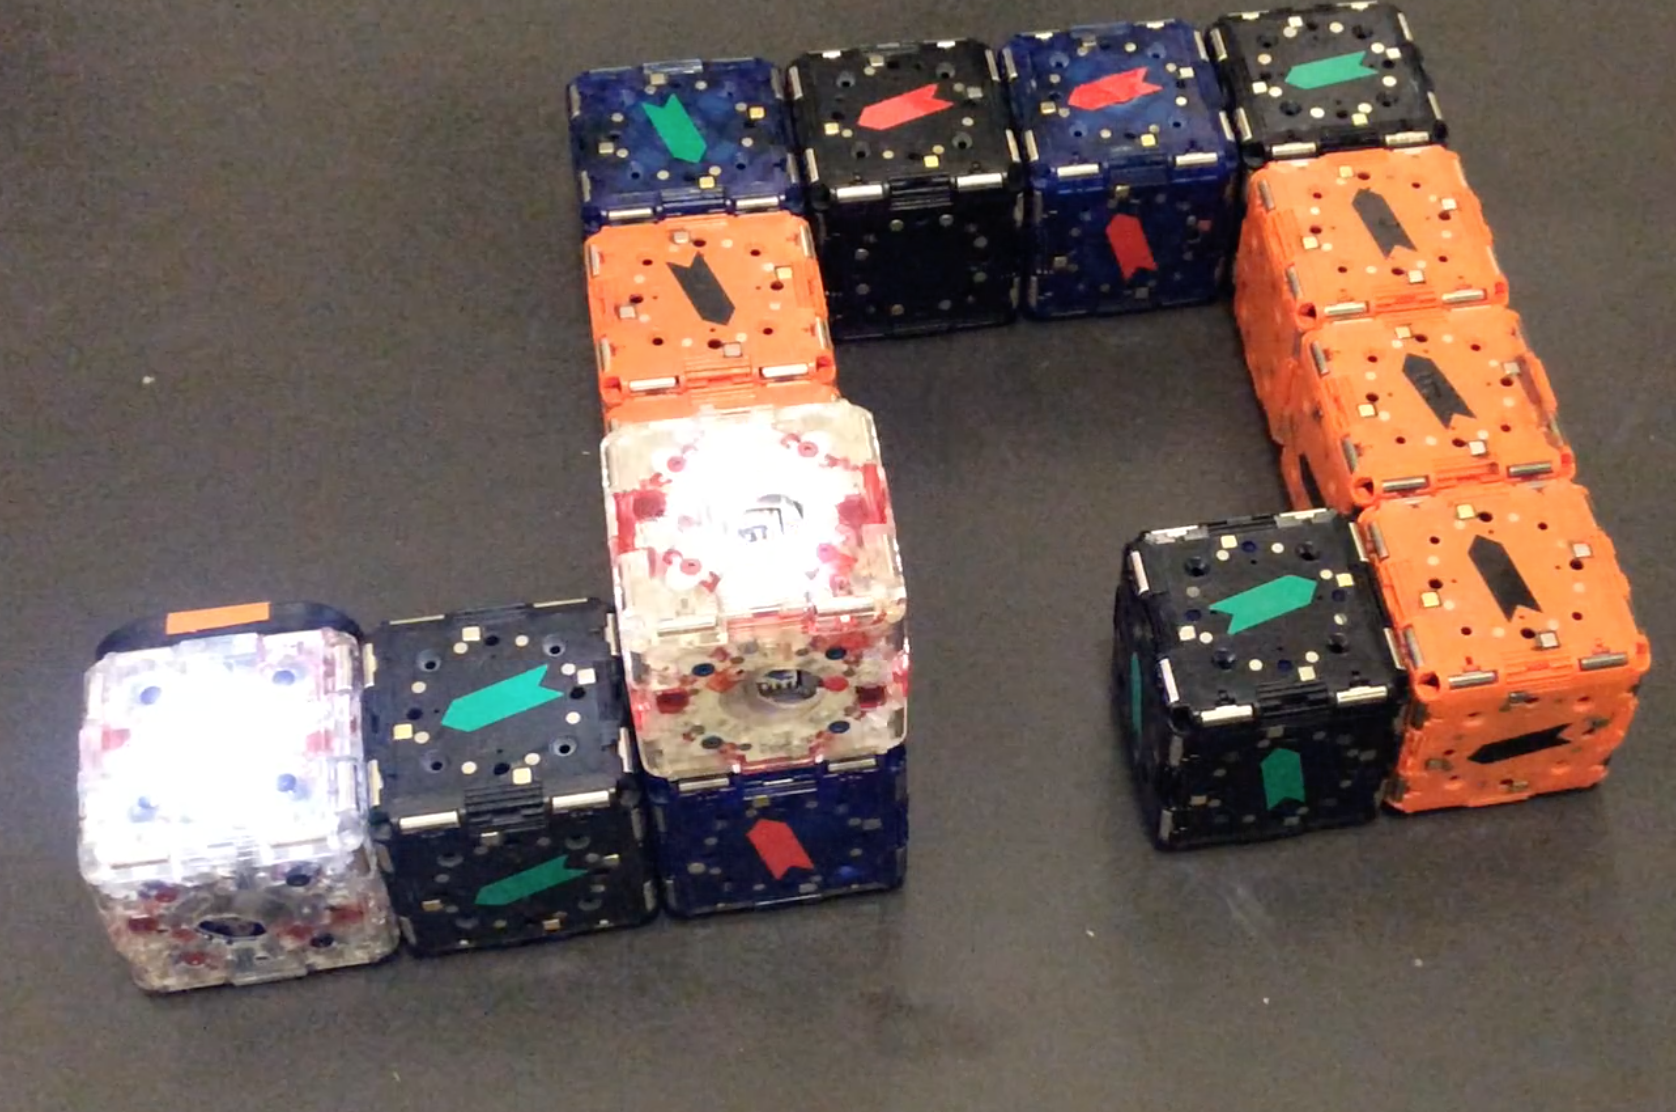
\includegraphics[width=0.97\linewidth]{figures/arrows_686.png}};
		\node[opacity = 0.5, fill = white, rounded corners] at (-0.25,-0.5) {t = 686 s};
		\end{tikzpicture}
	\end{subfigure}
	\begin{subfigure}[b]{0.30\linewidth}
		\begin{tikzpicture}[]	
		\node[opacity = 0.95] at (0,0) {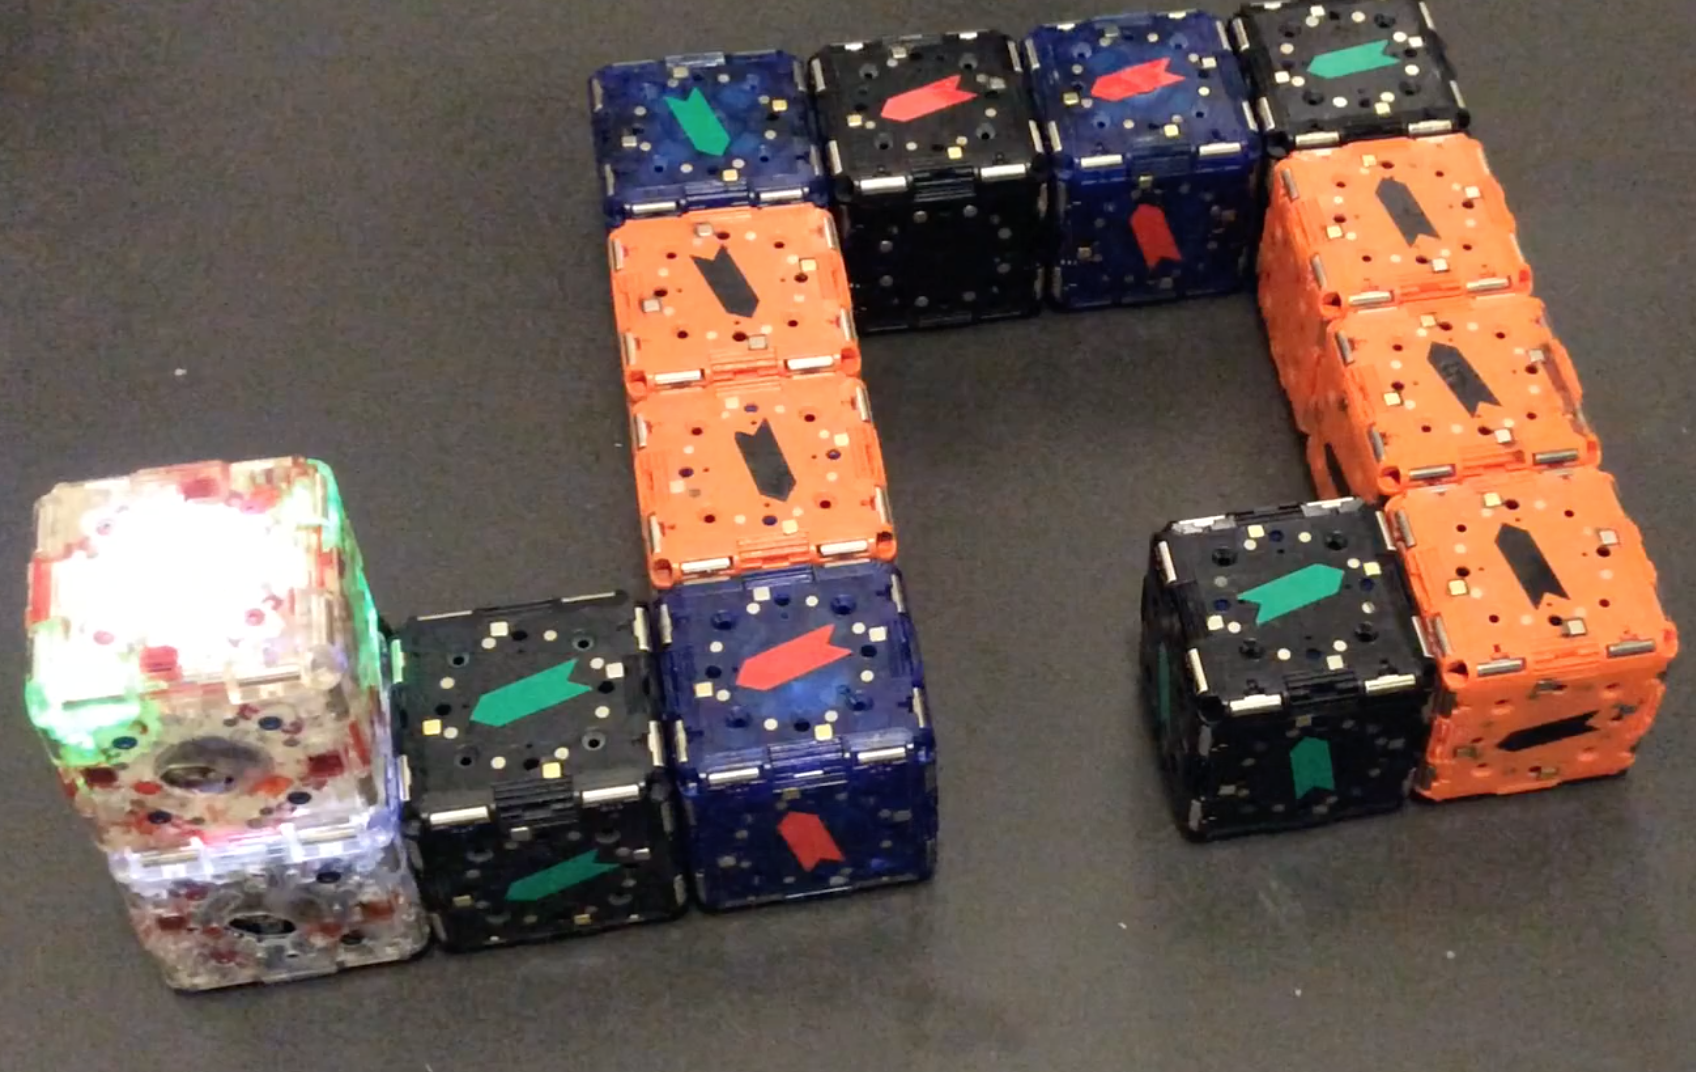
\includegraphics[width=0.97\linewidth]{figures/arrows_720.png}};
		\node[opacity = 0.5, fill = white, rounded corners] at (-0.25,-0.5) {t = 720 s};
		\end{tikzpicture}
	\end{subfigure}
%	\caption{In this experiment the module moves according to \tagNamePlural~embedded in passive modules. The module performing the experiment is preloaded with the angles for the tags with unique ID numbers, and apply these offsets in order to follow the path to the goal location.}
	\caption{In this experiment the module moves according to \tagNamePlural~embedded in passive modules. The module moves along the path until it connects to a module which has a LED turned on (the goal location).}
	
	\label{fig:arrowExperiment}
\end{figure}

%%%%%%%%%%%%%%%%%%%%%%%%%%%%%%%%%%%%%%%%%%%%%%%%%%%%%%%%%%%%%%%%%%%%%%%%%%%%%%%%%%%%%%%%%%%%%%%%%%%%%%%%%%%%%%%%%%%%%%%%%%%%%%%%%%%%%%%%%%%%%%%
%%%%%%%%%%%%%%%%%%%%%%%%%%%%%%%%%%%%%%%%%%%%%%%%%%%%%%%%%%%%%%%%%%%%%%%%%%%%%%%%%%%%%%%%%%%%%%%%%%%%%%%%%%%%%%%%%%%%%%%%%%%%%%%%%%%%%%%%%%%%%%%
\subsection{Line formation experiments}
\label{sec:mblocksExperimentsLine}
%%%%%%%%%%%%%%%%%%%%%%%%%%%%%%%%%%%%%%%%%%%%%%%%%%%%%%%%%%%%%%%%%%%%%%%%%%%%%%%%%%%%%%%%%%%%%%%%%%%%%%%%%%%%%%%%%%%%%%%%%%%%%%%%%%%%%%%%%%%%%%%
%%%%%%%%%%%%%%%%%%%%%%%%%%%%%%%%%%%%%%%%%%%%%%%%%%%%%%%%%%%%%%%%%%%%%%%%%%%%%%%%%%%%%%%%%%%%%%%%%%%%%%%%%%%%%%%%%%%%%%%%%%%%%%%%%%%%%%%%%%%%%%%

These experiments aimed to arbitrary 3D structures with constraints (no holes, and no modules connected by three or more connection faces) into a single horizontal line involving between 5 and 12 modules. These experiments were run with the aid a centralized WiFi server - whose function is to identify which module is the "seed" for the line. The server receives WiFi  status messages from the modules which includes their neighbors. The server attempts to find the longest existing line in the structure, and then picks one of the module closest to the center of that line, and sends a message to that module indicating that it is part of the line. 


\begin{figure}[h]  
	\centering
	\begin{subfigure}[b]{0.32\linewidth}
		\begin{tikzpicture}[]	
			\node[opacity = 0.95] at (0,0) {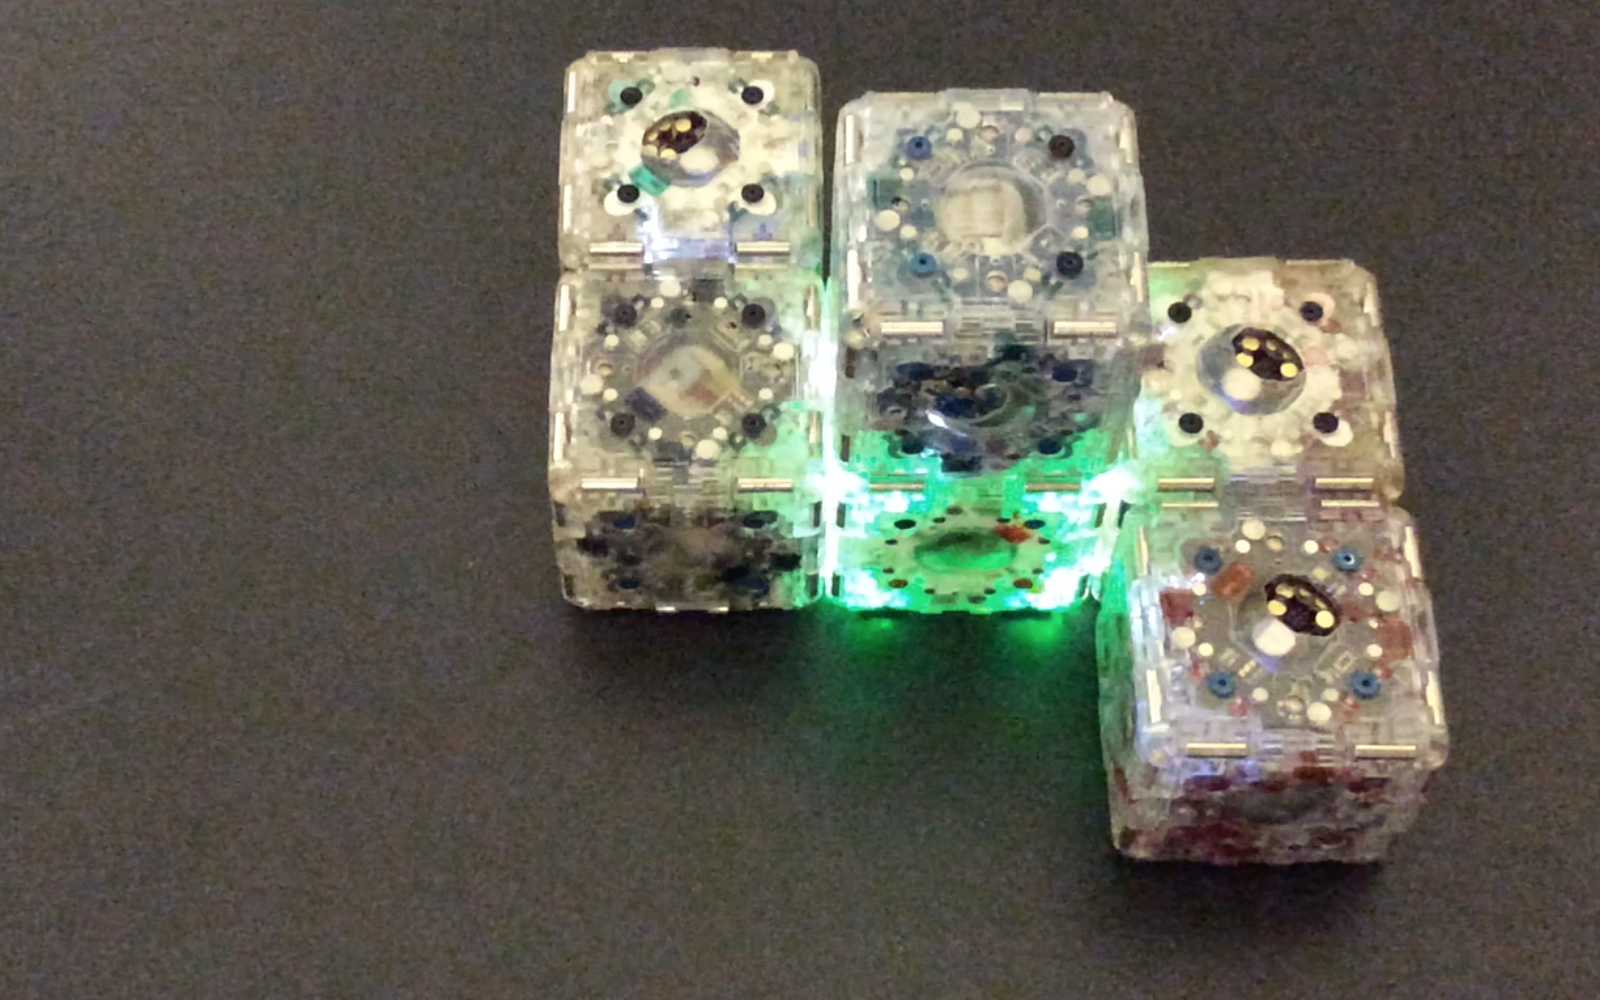
\includegraphics[width=0.95\linewidth]{figures/ActualLine_1.png}};
			\node[opacity = 0.5, fill = white, rounded corners] at (-0.5,-0.5) {t = 0 s};
		\end{tikzpicture} 
	\end{subfigure}
	\begin{subfigure}[b]{0.32\linewidth}
			\begin{tikzpicture}[]	
		\node[opacity = 0.95] at (0,0) {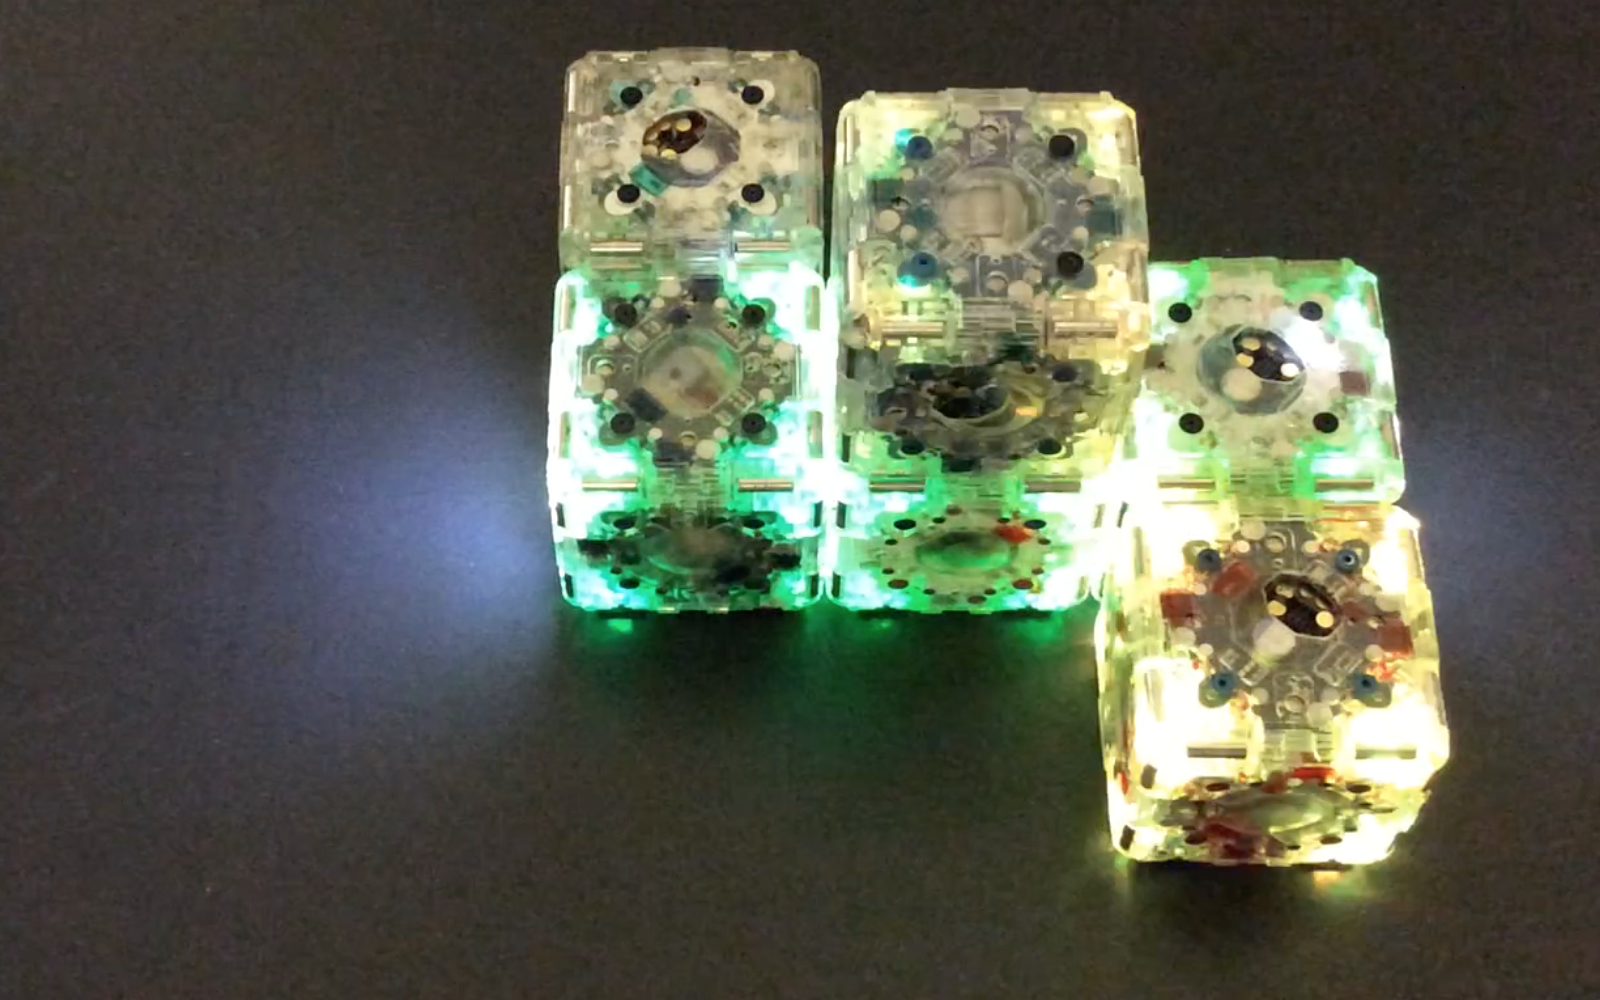
\includegraphics[width=0.95\linewidth]{figures/ActualLine_2.png}};
		\node[opacity = 0.5, fill = white, rounded corners] at (-0.5,-0.5) {t = 30 s};
		\end{tikzpicture}
	\end{subfigure}
	\begin{subfigure}[b]{0.32\linewidth}
			\begin{tikzpicture}[]	
		\node[opacity = 0.95] at (0,0) {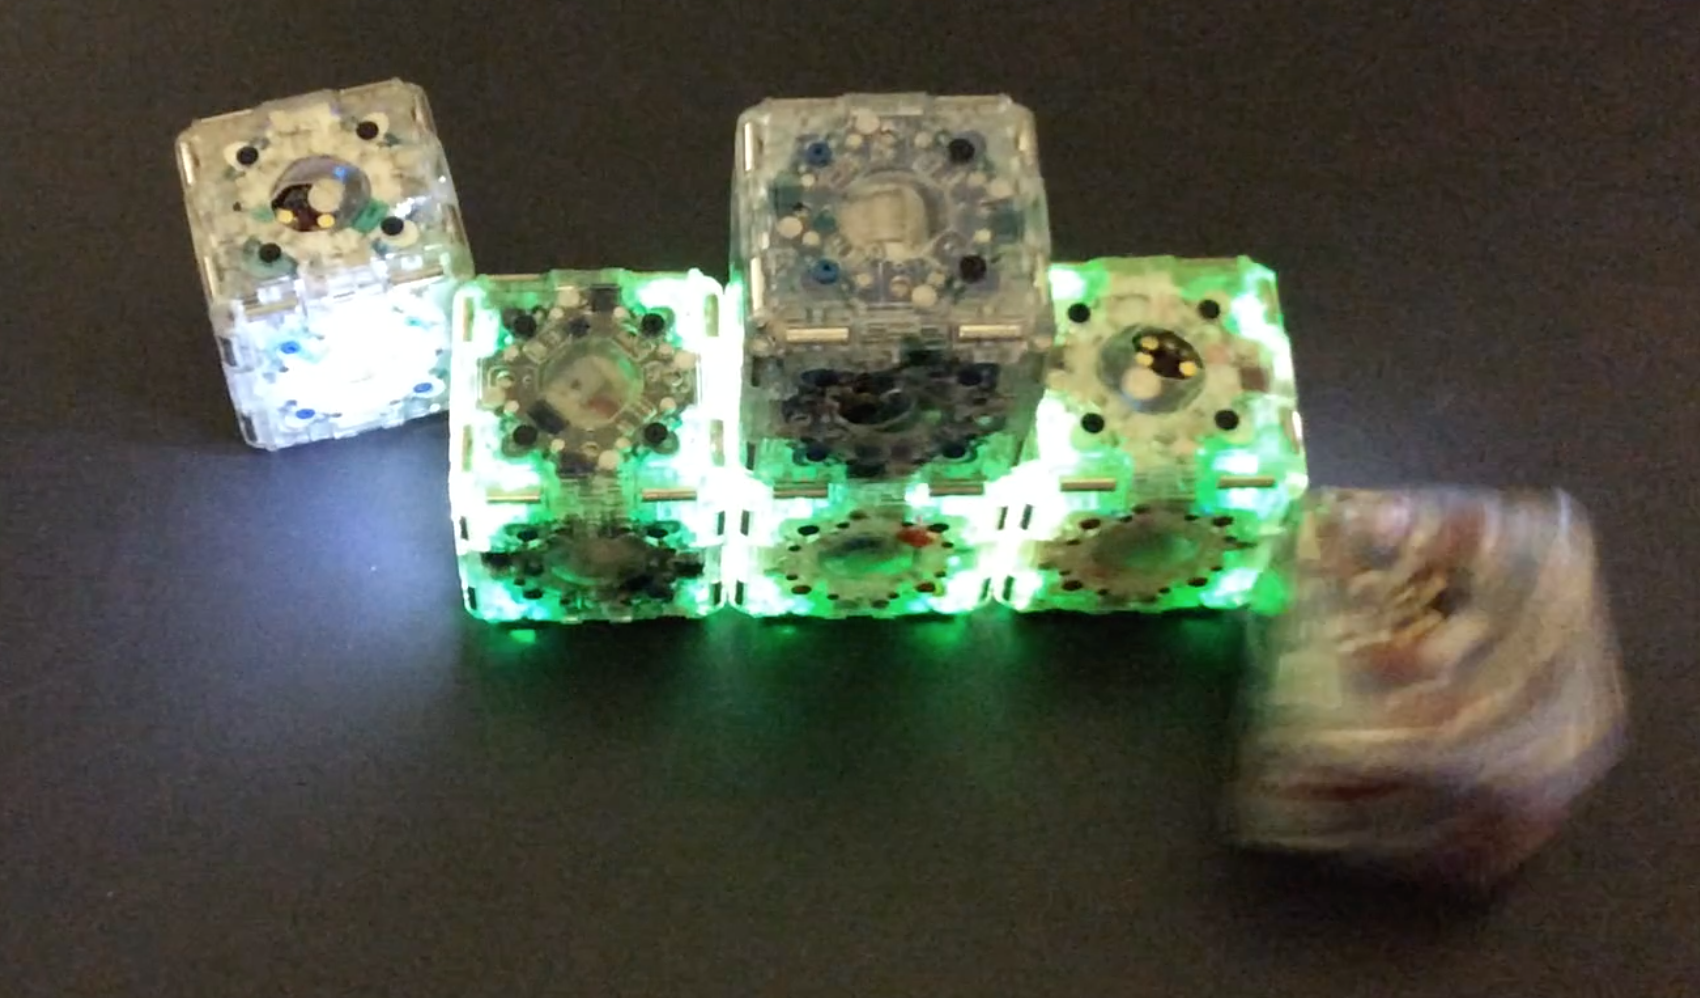
\includegraphics[width=0.95\linewidth]{figures/ActualLine_3.png}};
		\node[opacity = 0.5, fill = white, rounded corners] at (-0.5,-0.5) {t = 60 s};
		\end{tikzpicture}
	\end{subfigure}

	\begin{subfigure}[b]{0.32\linewidth}
			\begin{tikzpicture}[]	
		\node[opacity = 0.95] at (0,0) {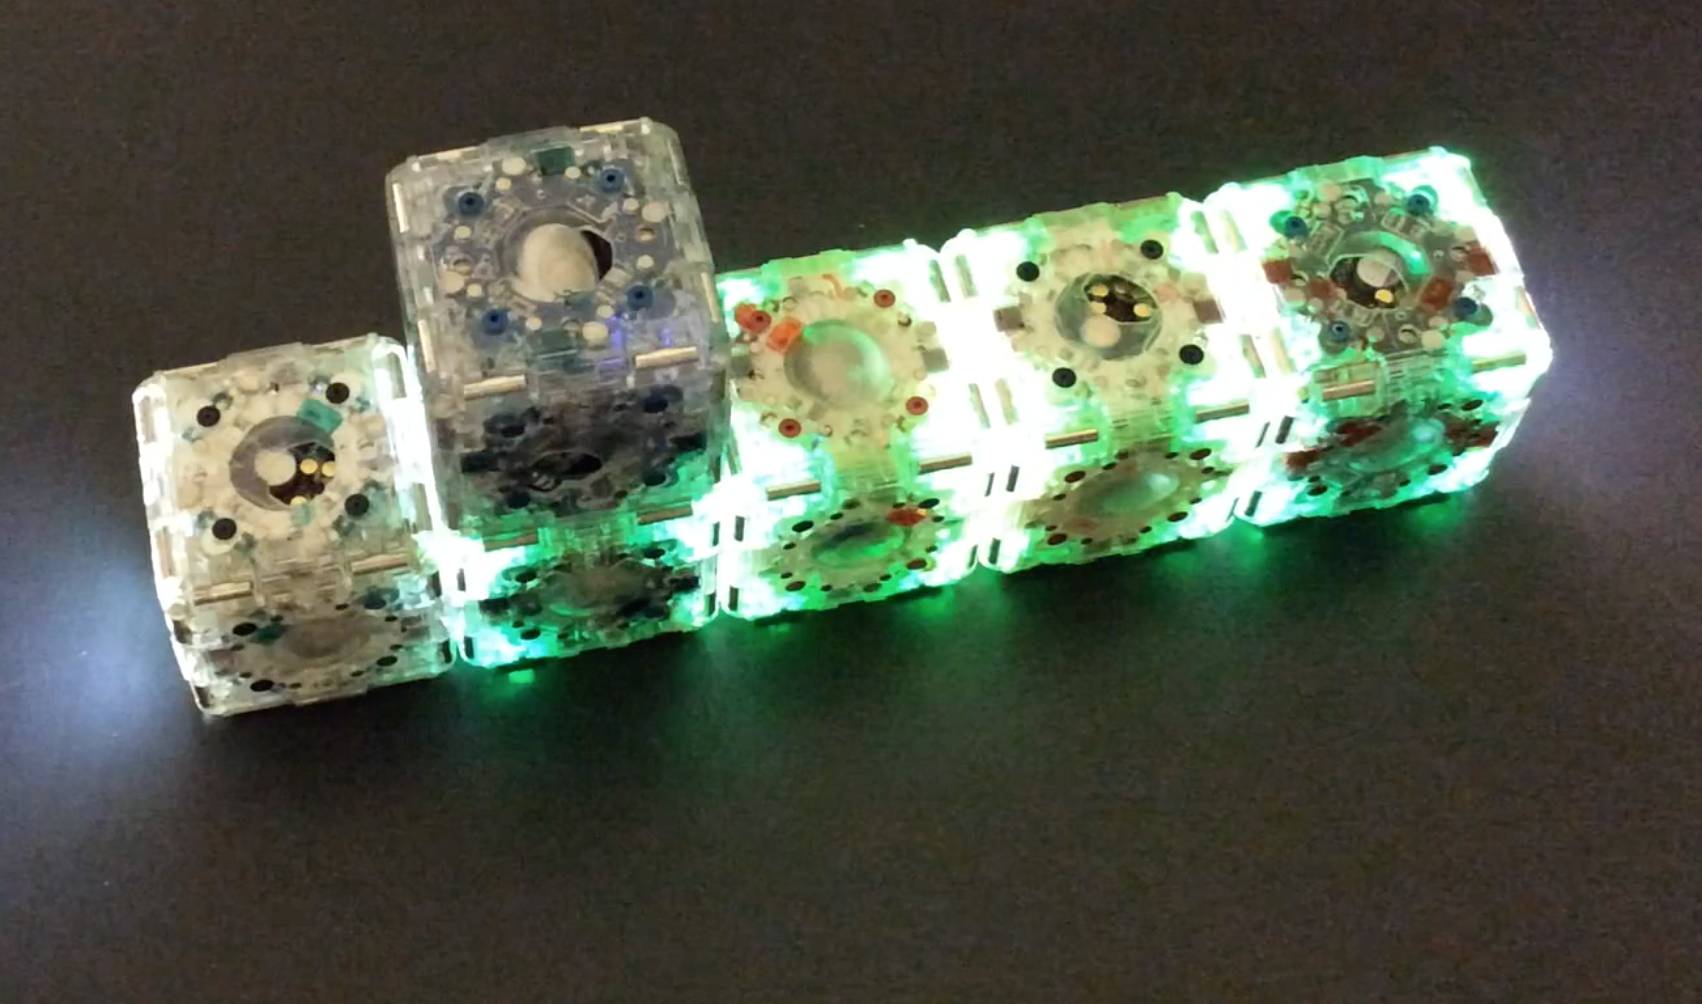
\includegraphics[width=0.95\linewidth]{figures/ActualLine_4.png}};
		\node[opacity = 0.5, fill = white, rounded corners] at (-0.5,-0.5) {t = 120 s};
		\end{tikzpicture}
	\end{subfigure}
	\begin{subfigure}[b]{0.32\linewidth}
			\begin{tikzpicture}[]	
		\node[opacity = 0.95] at (0,0) {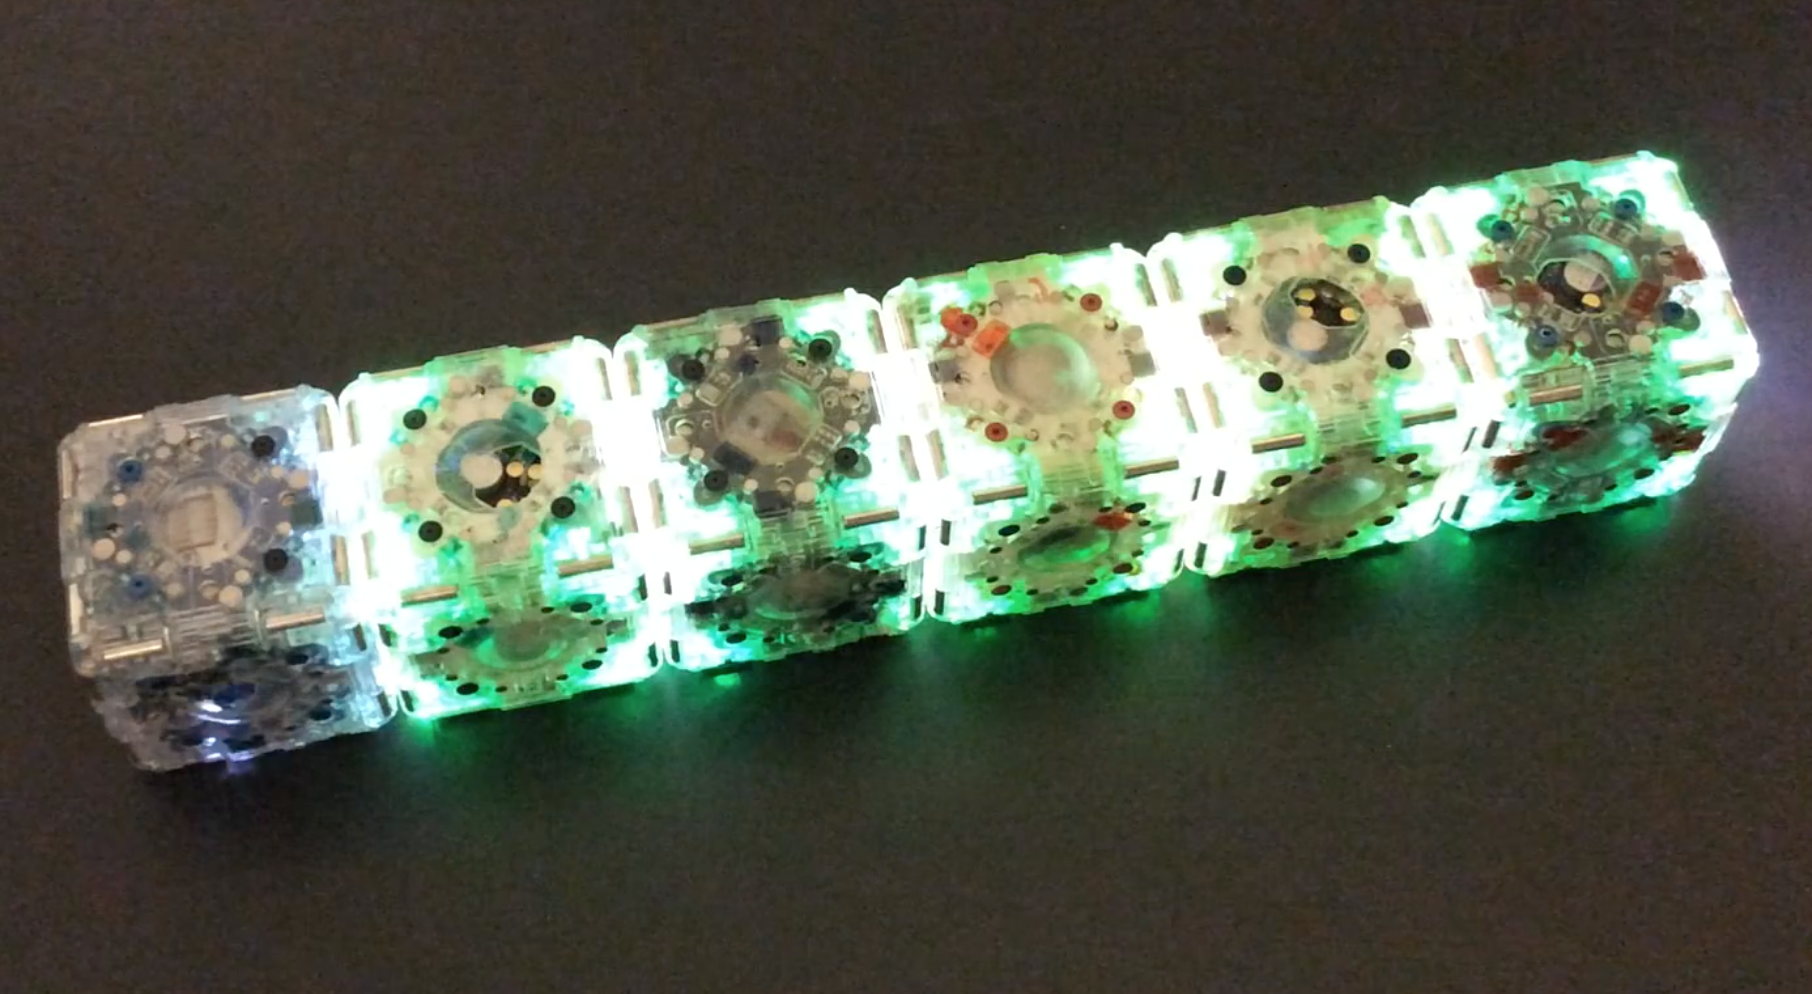
\includegraphics[width=0.95\linewidth]{figures/ActualLine_5.png}};
		\node[opacity = 0.5, fill = white, rounded corners] at (-0.5,-0.5) {t = 230 s};
		\end{tikzpicture}
	\end{subfigure}
	\begin{subfigure}[b]{0.32\linewidth}
			\begin{tikzpicture}[]	
		\node[opacity = 0.95] at (0,0) {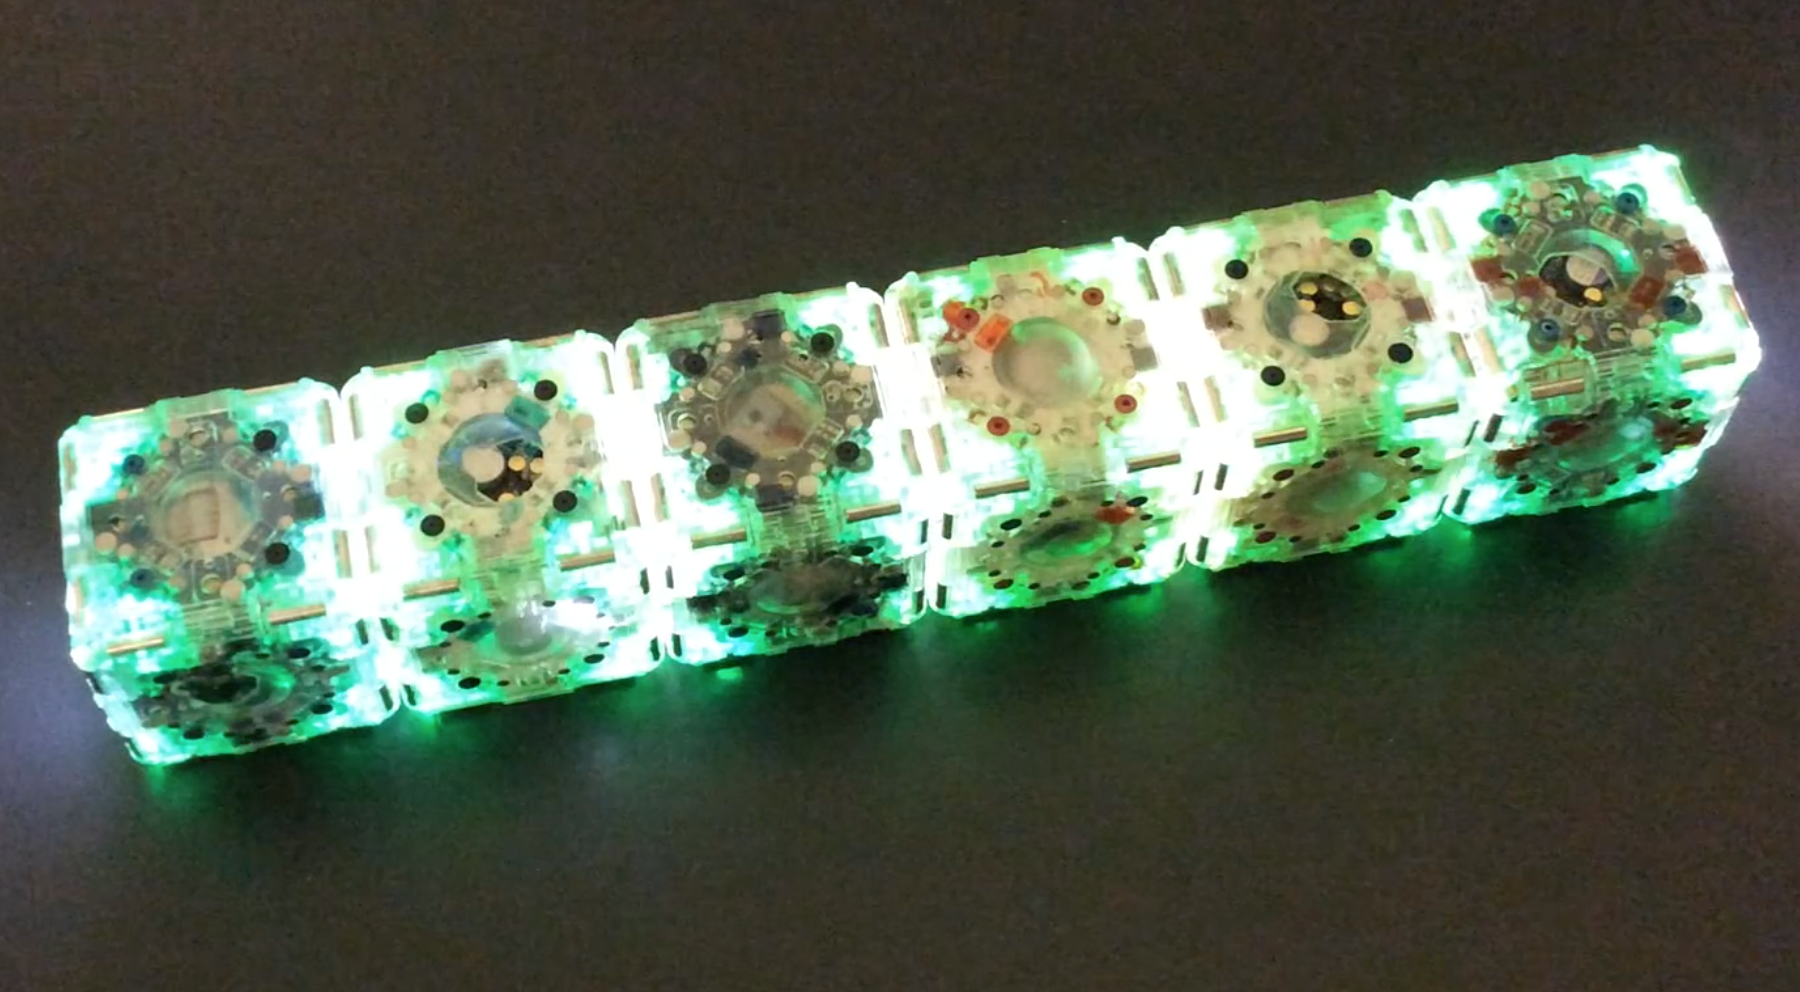
\includegraphics[width=0.95\linewidth]{figures/ActualLine_6.png}};
		\node[opacity = 0.5, fill = white, rounded corners] at (-0.5,-0.5) {t = 300 s};
		\end{tikzpicture}
	\end{subfigure}
	
	\caption{This experiment shows an arbitrary 3D configuration of M-Blocks reconfiguring into a line.}
	
	\label{fig:lineExperiment}
\end{figure}

%%%%%%%%%%%%%%%%%%%%%%%%%%%%%%%%%%%%%%%%%%%%%%%%%%%%%%%%%%%%%%%%%%%%%%%%%%%%%%%%%%%%%%%%%%%%%%%%%%%%%%%%%%%%%%%%%%%%%%%%%%%%%%%%%%%%%%%%%%%%%%%
%%%%%%%%%%%%%%%%%%%%%%%%%%%%%%%%%%%%%%%%%%%%%%%%%%%%%%%%%%%%%%%%%%%%%%%%%%%%%%%%%%%%%%%%%%%%%%%%%%%%%%%%%%%%%%%%%%%%%%%%%%%%%%%%%%%%%
\subsection{Light guided aggregation experiments}
\label{sec:mblocksExperimentsLight}
%%%%%%%%%%%%%%%%%%%%%%%%%%%%%%%%%%%%%%%%%%%%%%%%%%%%%%%%%%%%%%%%%%%%%%%%%%%%%%%%%%%%%%%%%%%%%%%%%%%%%%%%%%%%%%%%%%%%%%%%%%%%%%%%%%%%%%%%%%%%%%%
%%%%%%%%%%%%%%%%%%%%%%%%%%%%%%%%%%%%%%%%%%%%%%%%%%%%%%%%%%%%%%%%%%%%%%%%%%%%%%%%%%%%%%%%%%%%%%%%%%%%%%%%%%%%%%%%%%%%%%%%%%%%%%%%%%%%%%%%%%%%%%%


These experiments implement the photo-taxis Braitenberg behavior for a group of M-Blocks modules. There is a single light source, and a special target module, which when modules aggregate to it, the modules share its location through wireless and light signals for additional modules to connect to it - essentially forming a single "crystal" of aggregated modules. In these experiment modules are gradually released into a confined (0.5m x 0.5 m) bounded foam-padded location, and move until they either run out of battery or connect to the designated aggregate.

%\newcommand{\figureWidth}{0.32\linewidth}
\begin{figure}[h]  
	\centering
	\begin{subfigure}[b]{0.32\linewidth}
		
		\begin{tikzpicture}[]	
			\node[opacity = 0.95] at (0,0) {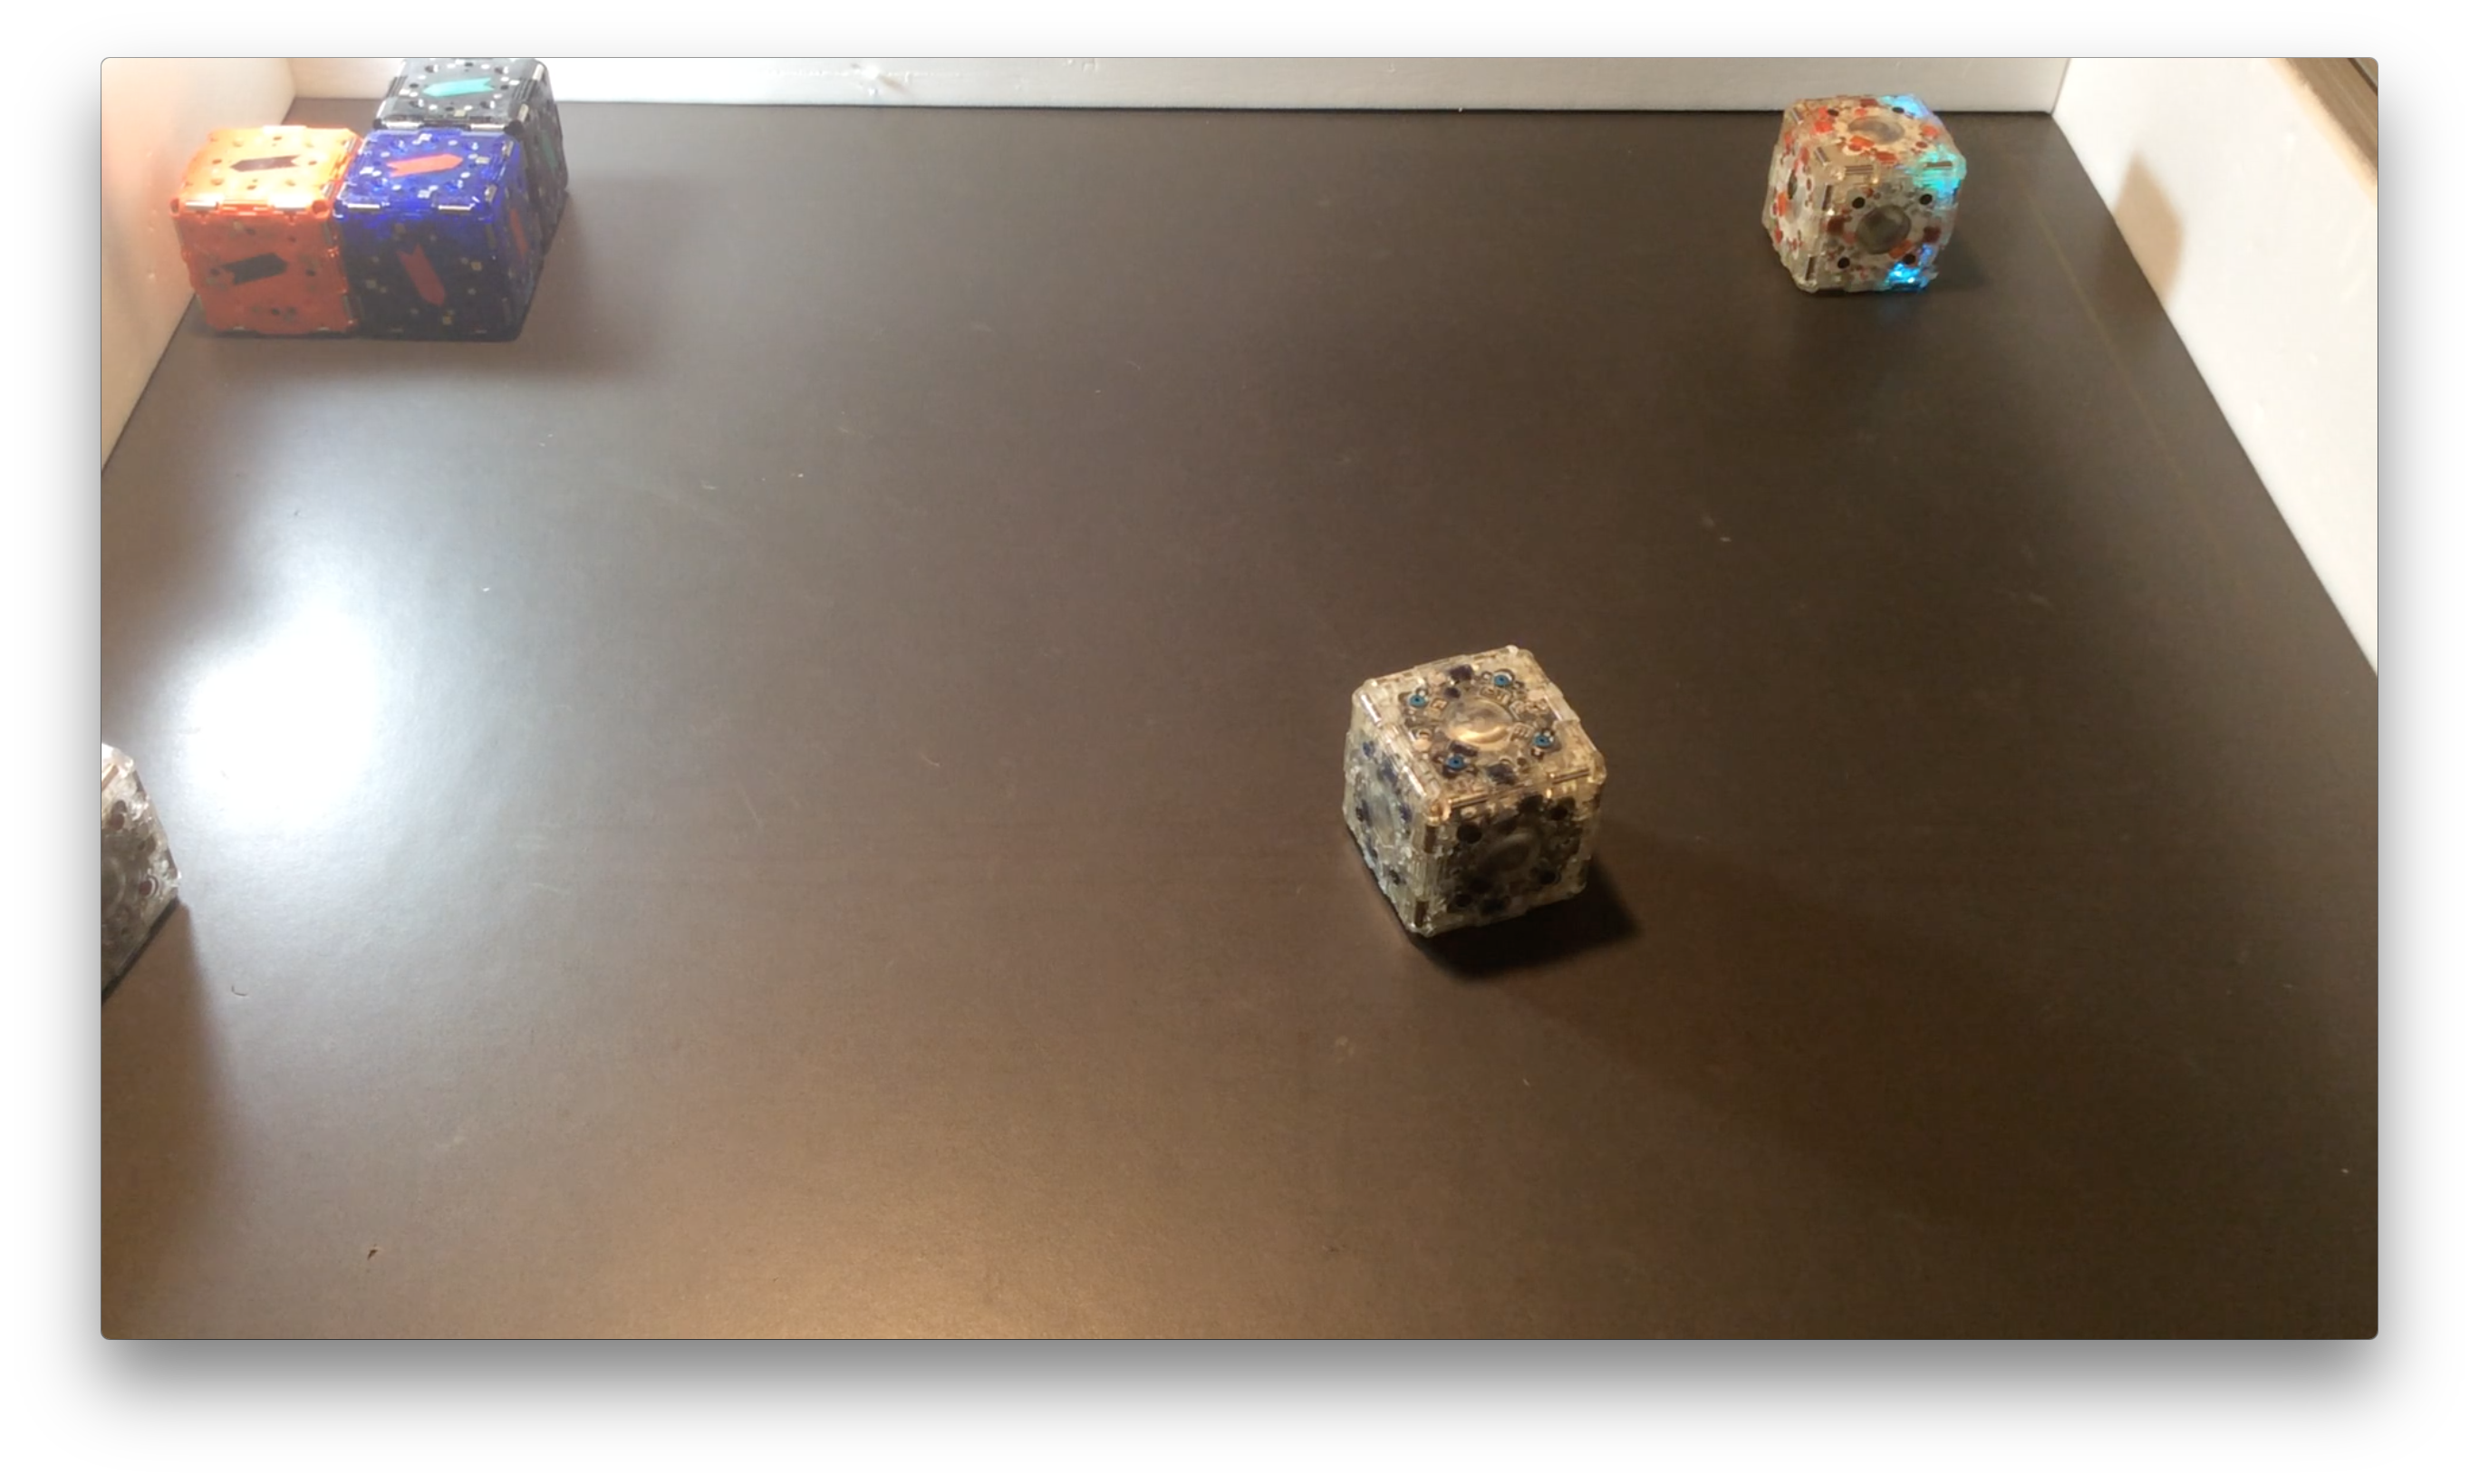
\includegraphics[width = \linewidth]{figures/1-000.png}};
			\node[opacity = 0.5, fill = white, rounded corners] at (-0.5,-0.5) {t = 000 s};
		\end{tikzpicture}
		
	\end{subfigure}
	\begin{subfigure}[b]{0.32\linewidth}
		
		\begin{tikzpicture}[]	
		\node[opacity = 0.95] at (0,0) {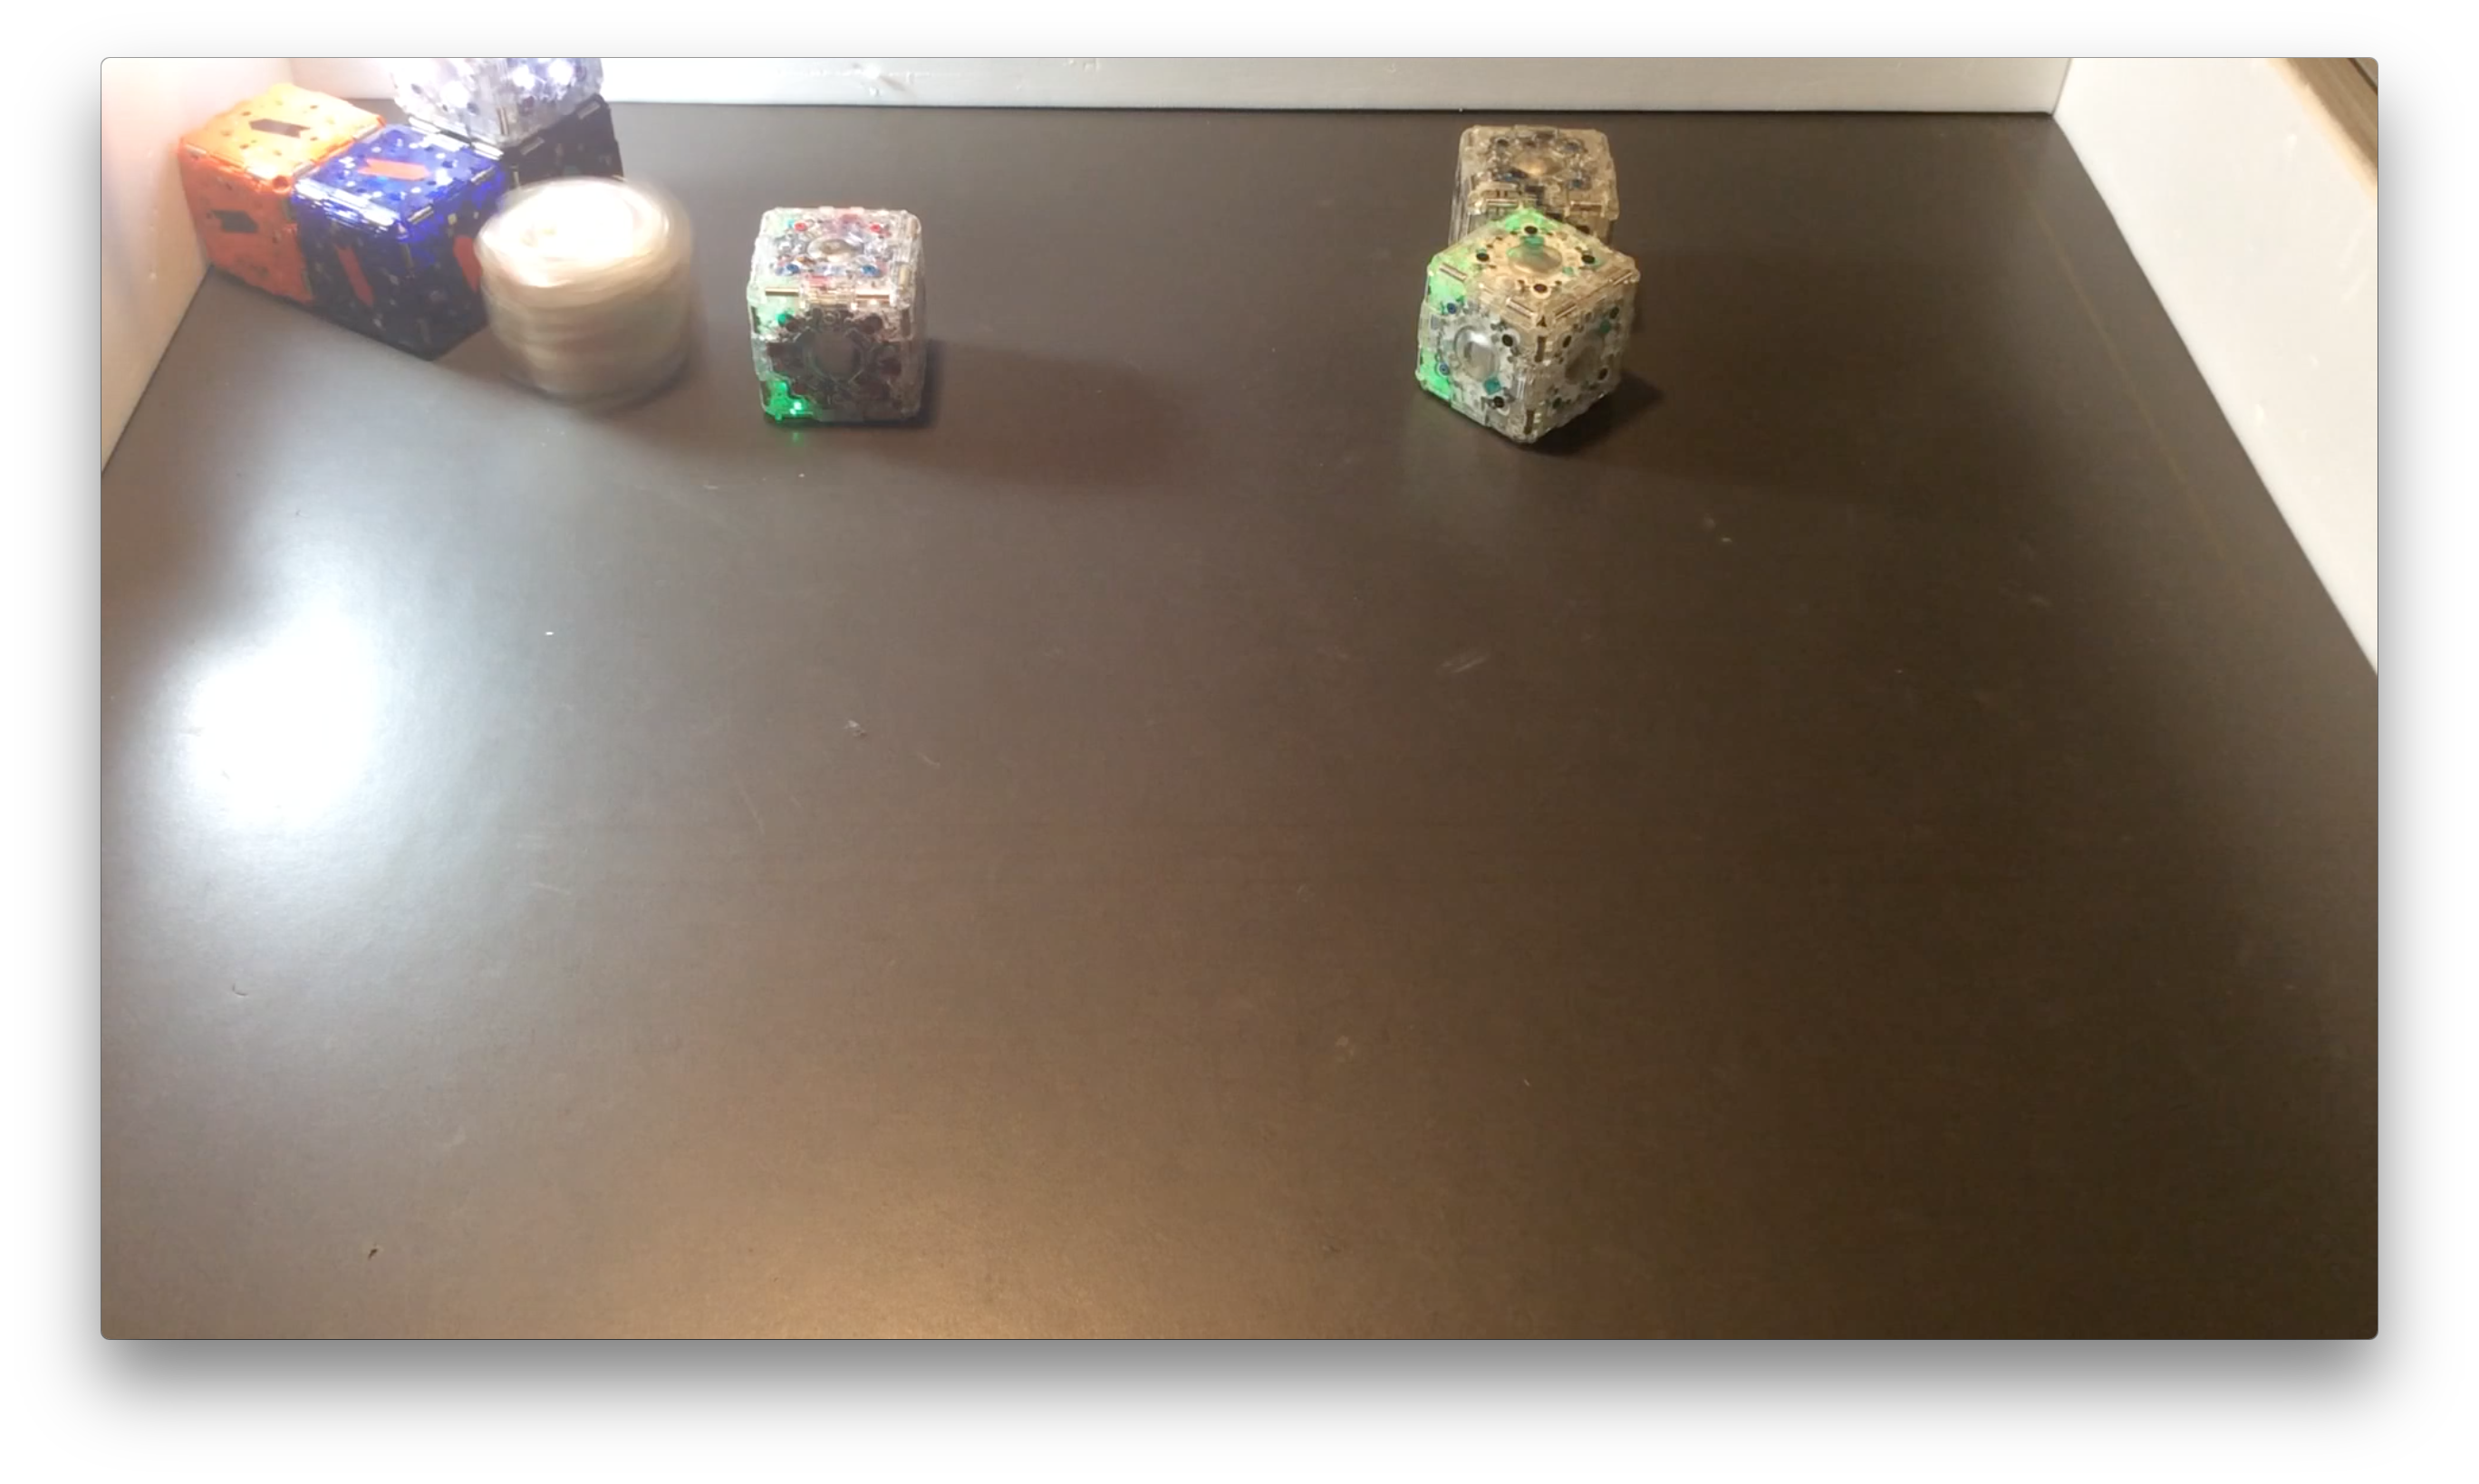
\includegraphics[width = \linewidth]{figures/2-120.png}};
		\node[opacity = 0.5, fill = white, rounded corners] at (-0.5,-0.5) {t = 120 s};
		\end{tikzpicture}
		
	\end{subfigure}
	\begin{subfigure}[b]{0.32\linewidth}

		\begin{tikzpicture}[]	
		\node[opacity = 0.95] at (0,0) {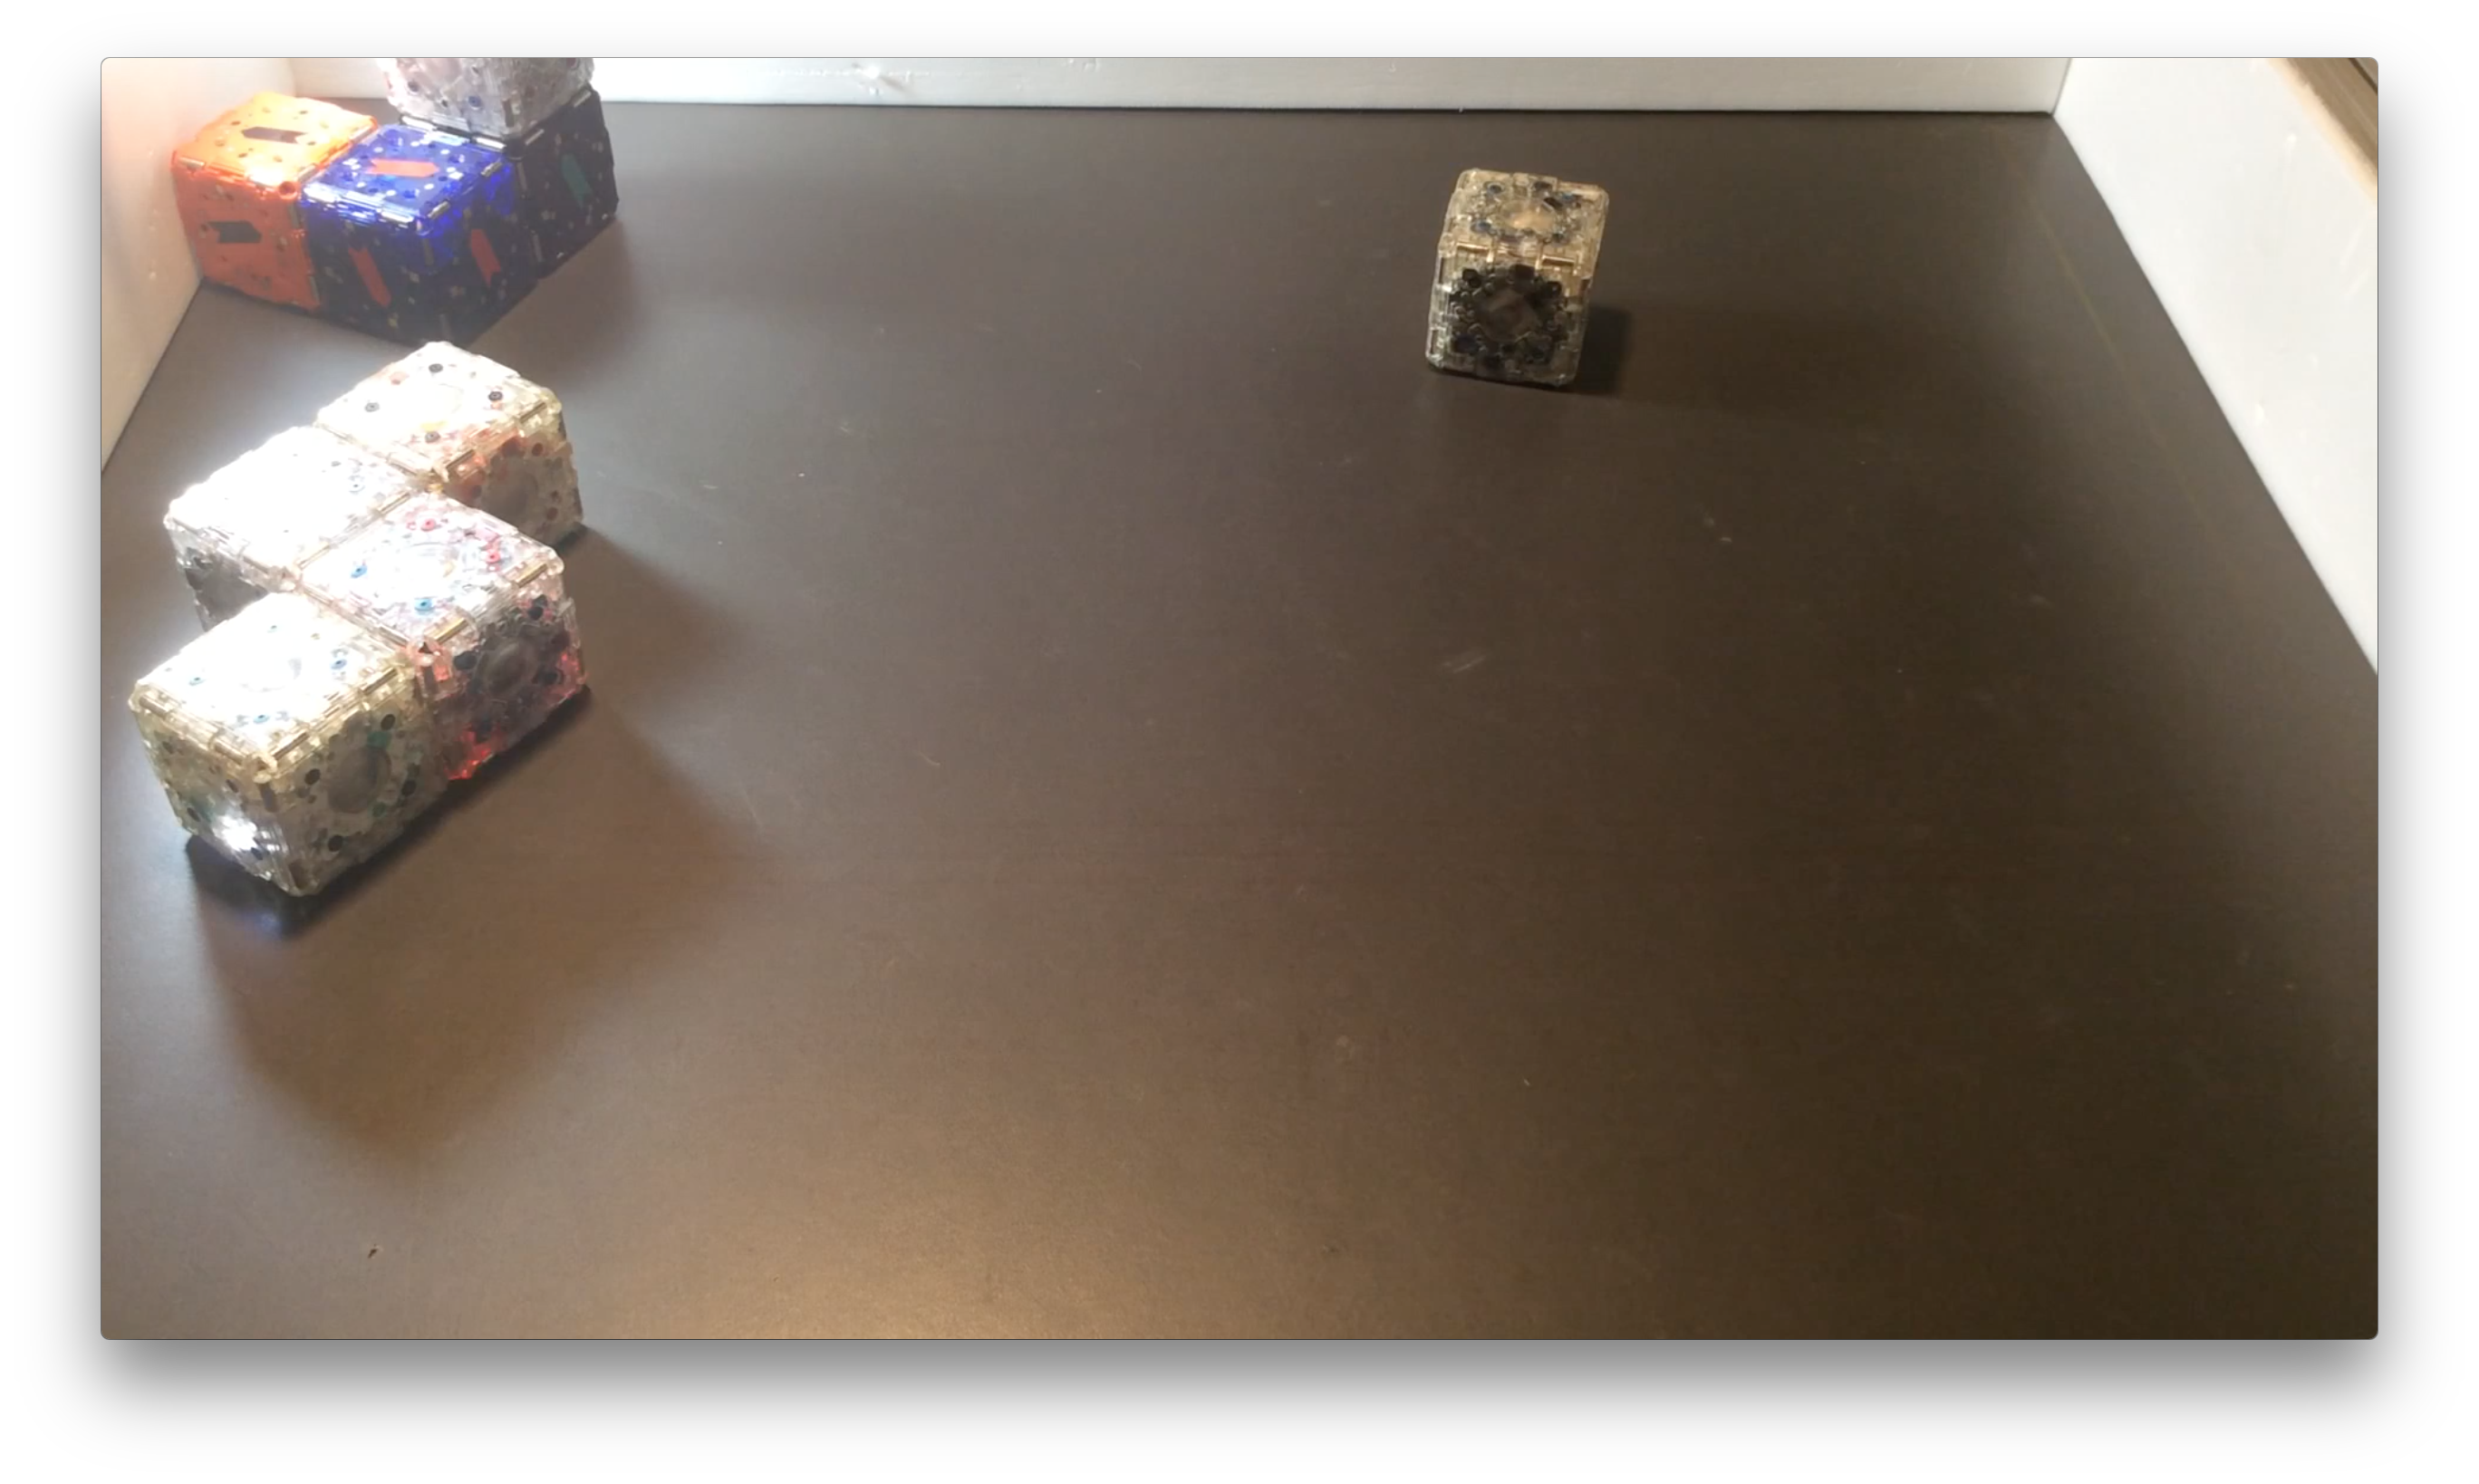
\includegraphics[width = \linewidth]{figures/3-220.png}};
		\node[opacity = 0.5, fill = white, rounded corners] at (-0.5,-0.5) {t = 220 s};
		\end{tikzpicture}
		
	\end{subfigure}

	\begin{subfigure}[b]{0.32\linewidth}
		\begin{tikzpicture}[]	
		\node[opacity = 0.95] at (0,0) {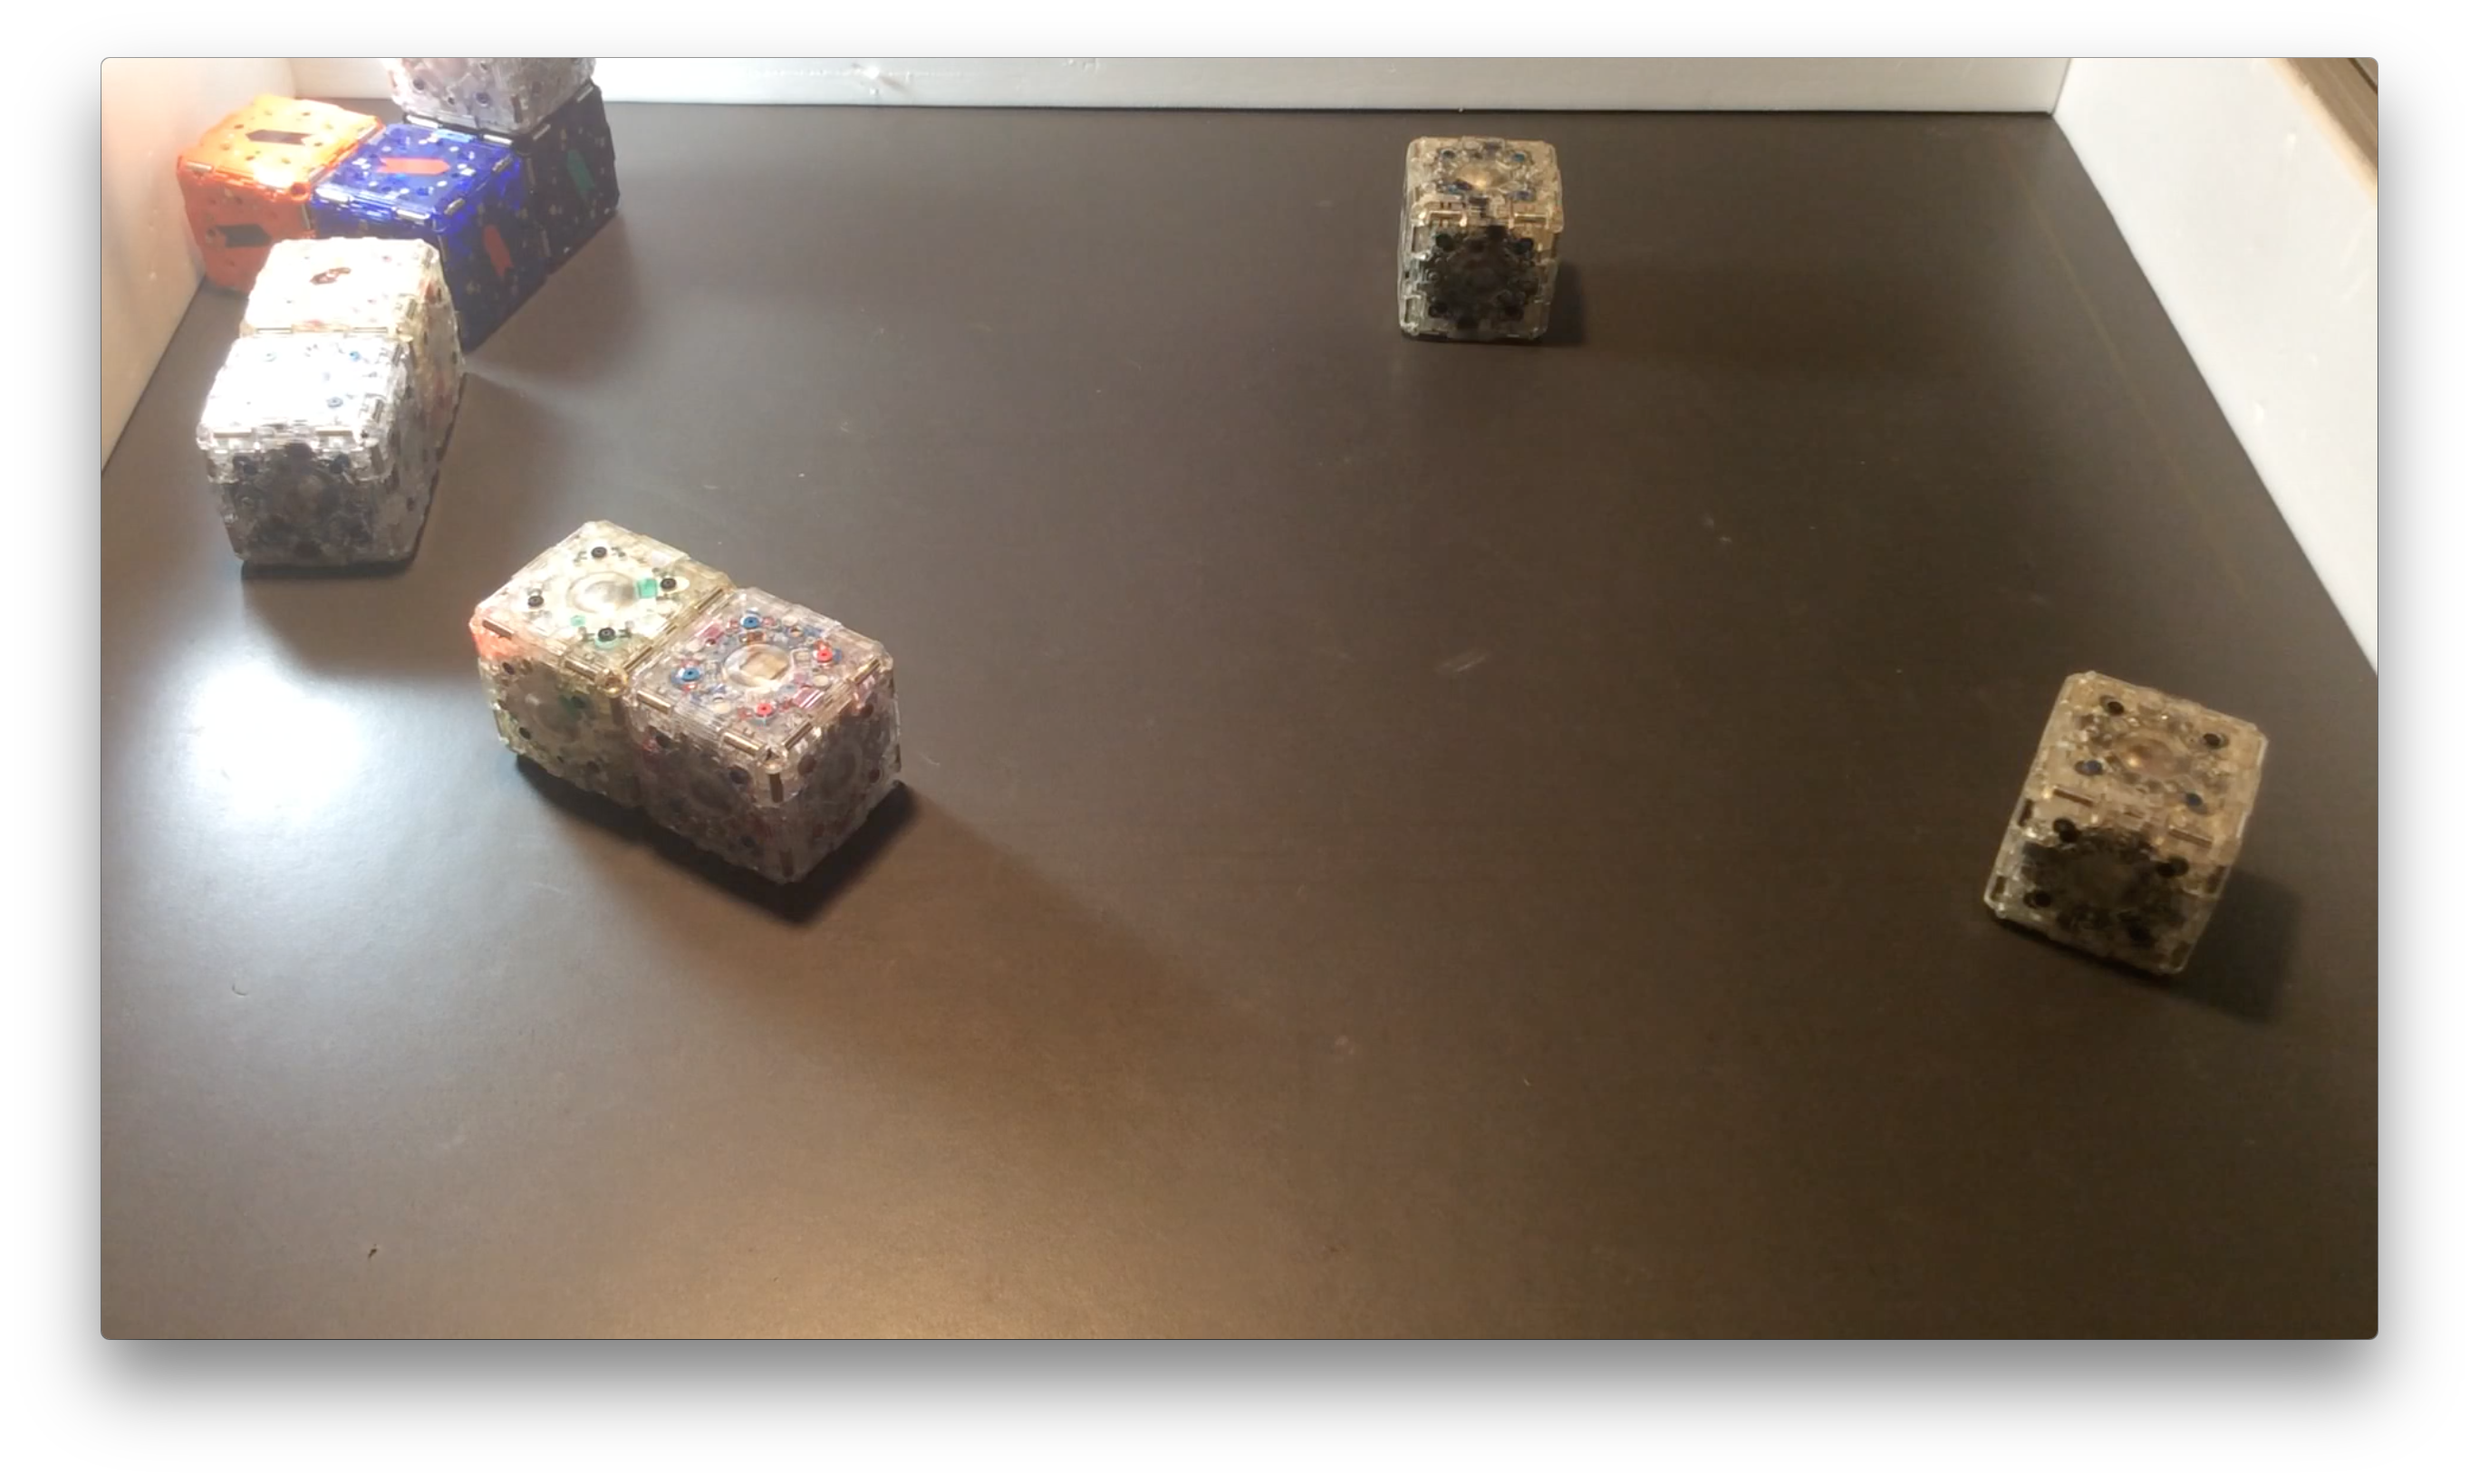
\includegraphics[width = \linewidth]{figures/4-320.png}};
		\node[opacity = 0.5, fill = white, rounded corners] at (-0.5,-0.5) {t = 320 s};
		\end{tikzpicture}
	\end{subfigure}
	\begin{subfigure}[b]{0.32\linewidth}
		\begin{tikzpicture}[]	
		\node[opacity = 0.95] at (0,0) {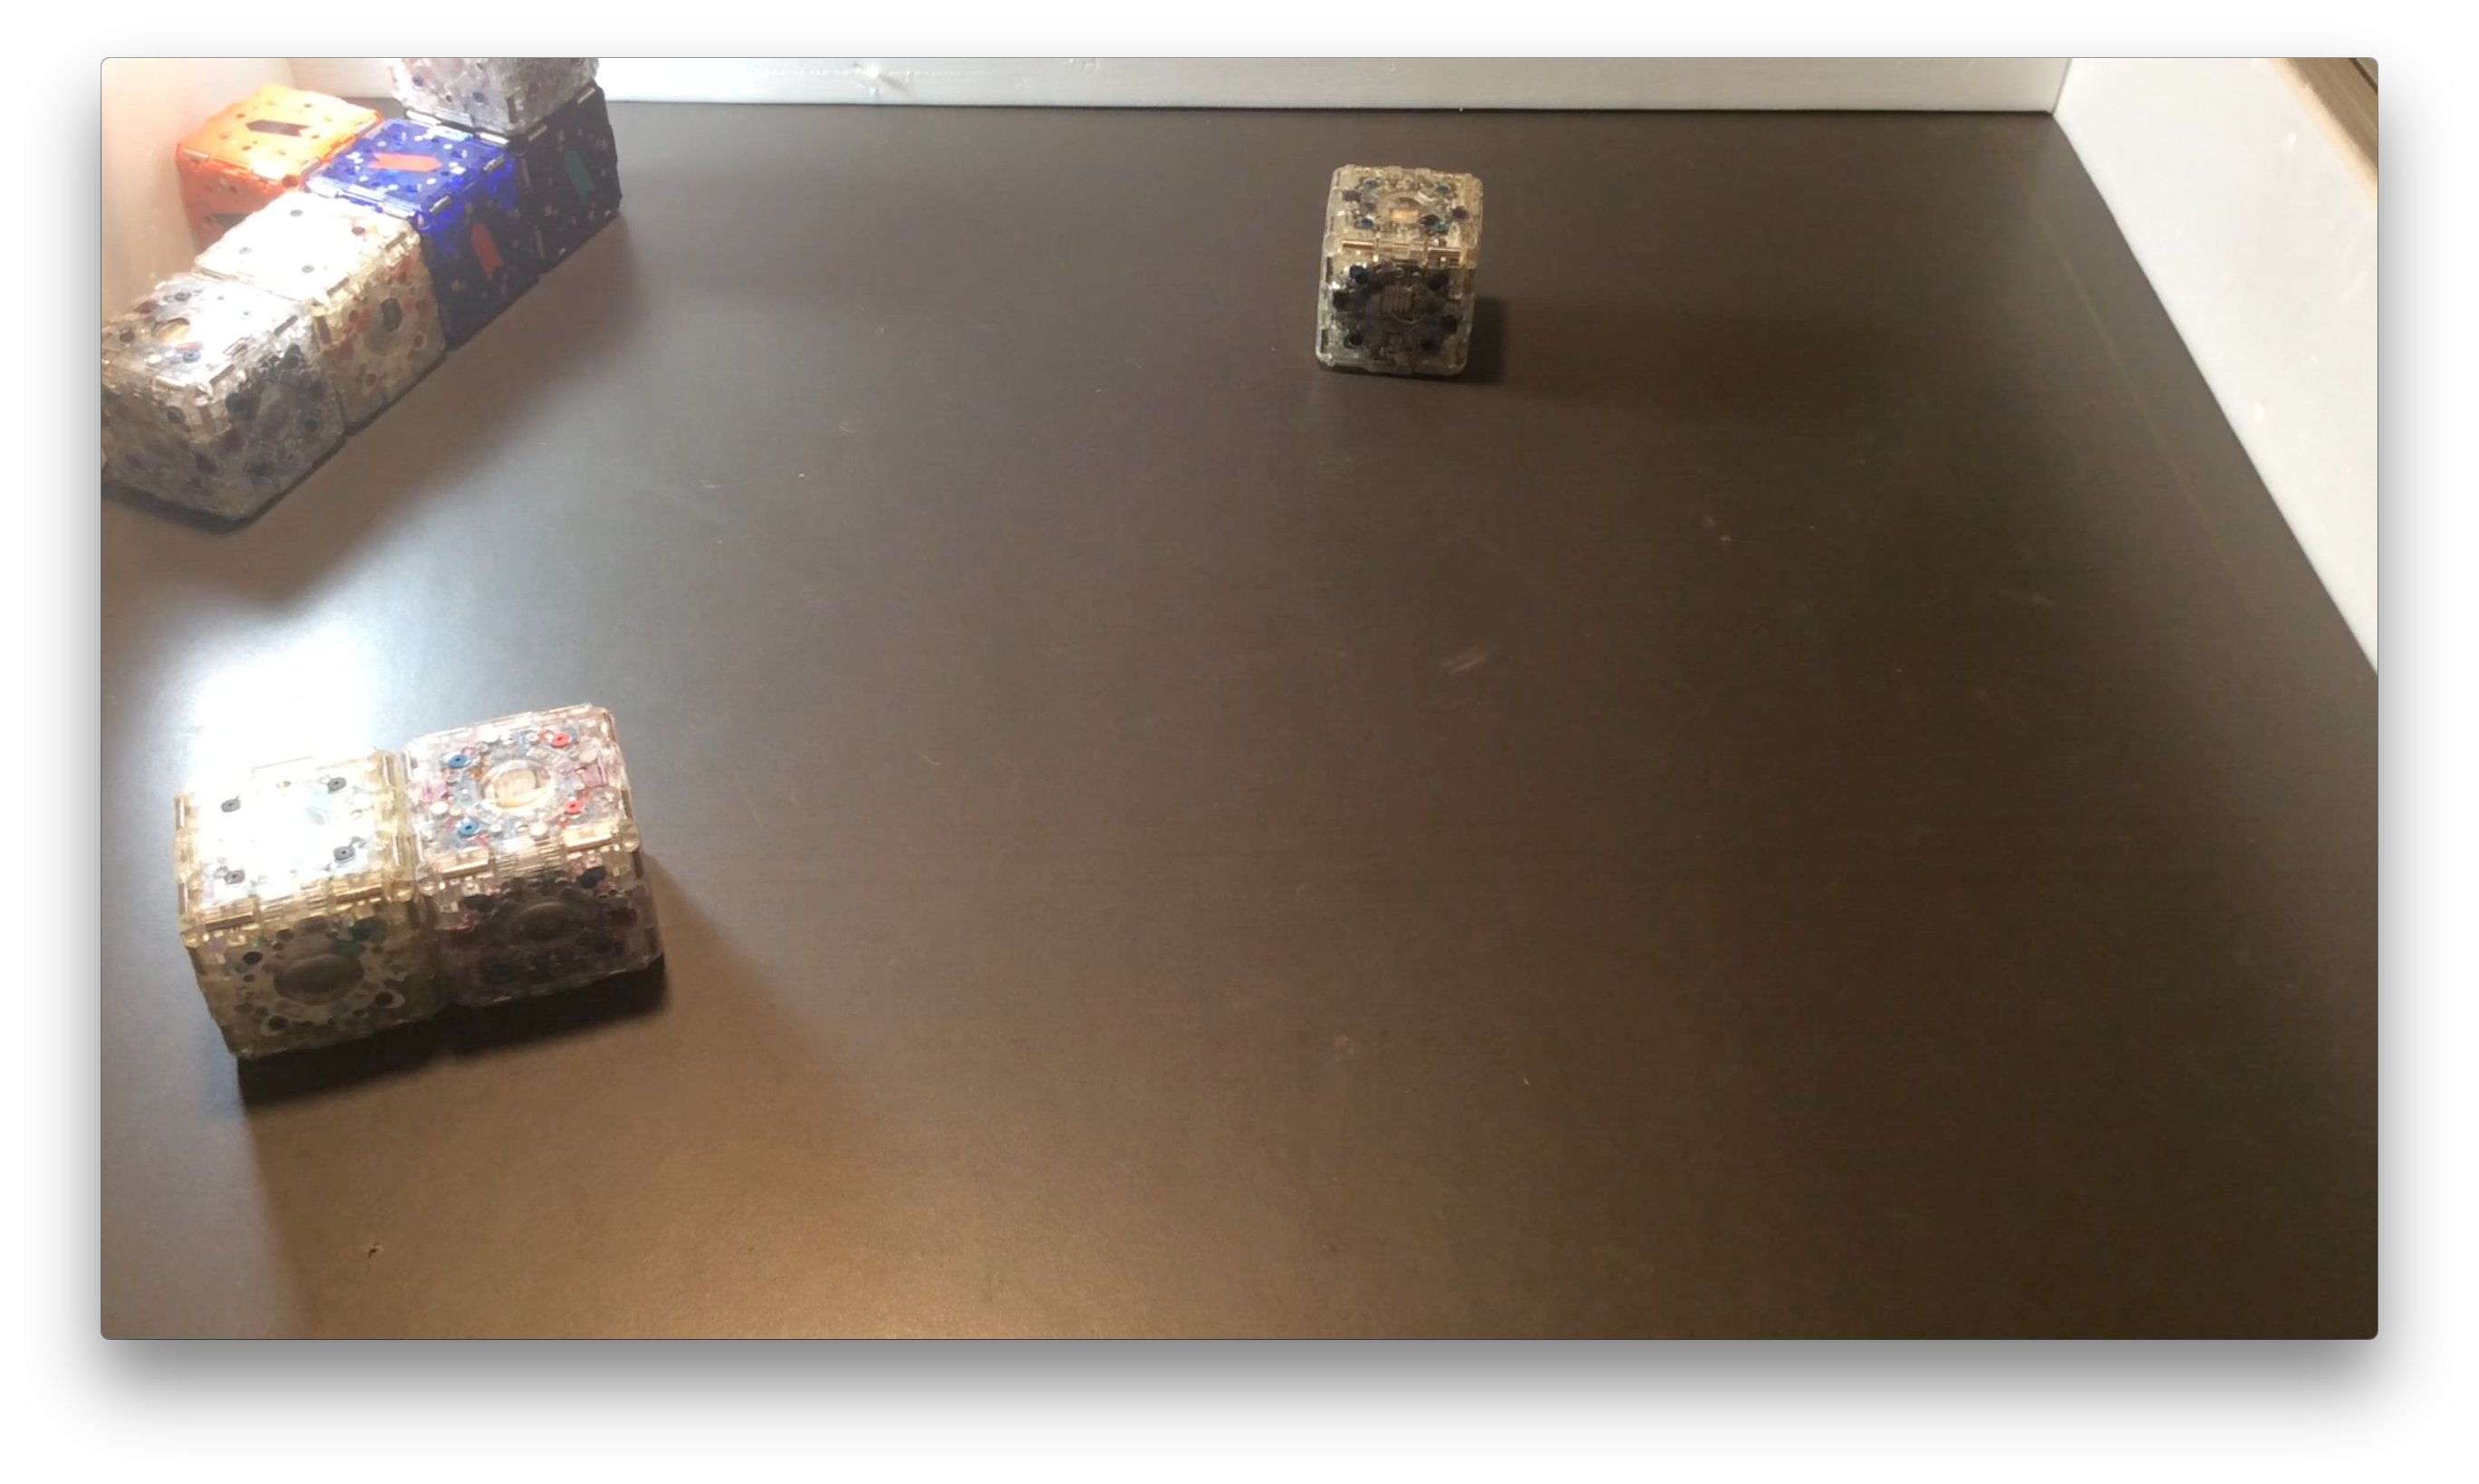
\includegraphics[width = \linewidth]{figures/5-500.png}};
		\node[opacity = 0.5, fill = white, rounded corners] at (-0.5,-0.5) {t = 500 s};
		\end{tikzpicture} 
	\end{subfigure}
	\begin{subfigure}[b]{0.32\linewidth}
		\begin{tikzpicture}[]	
		\node[opacity = 0.95] at (0,0) {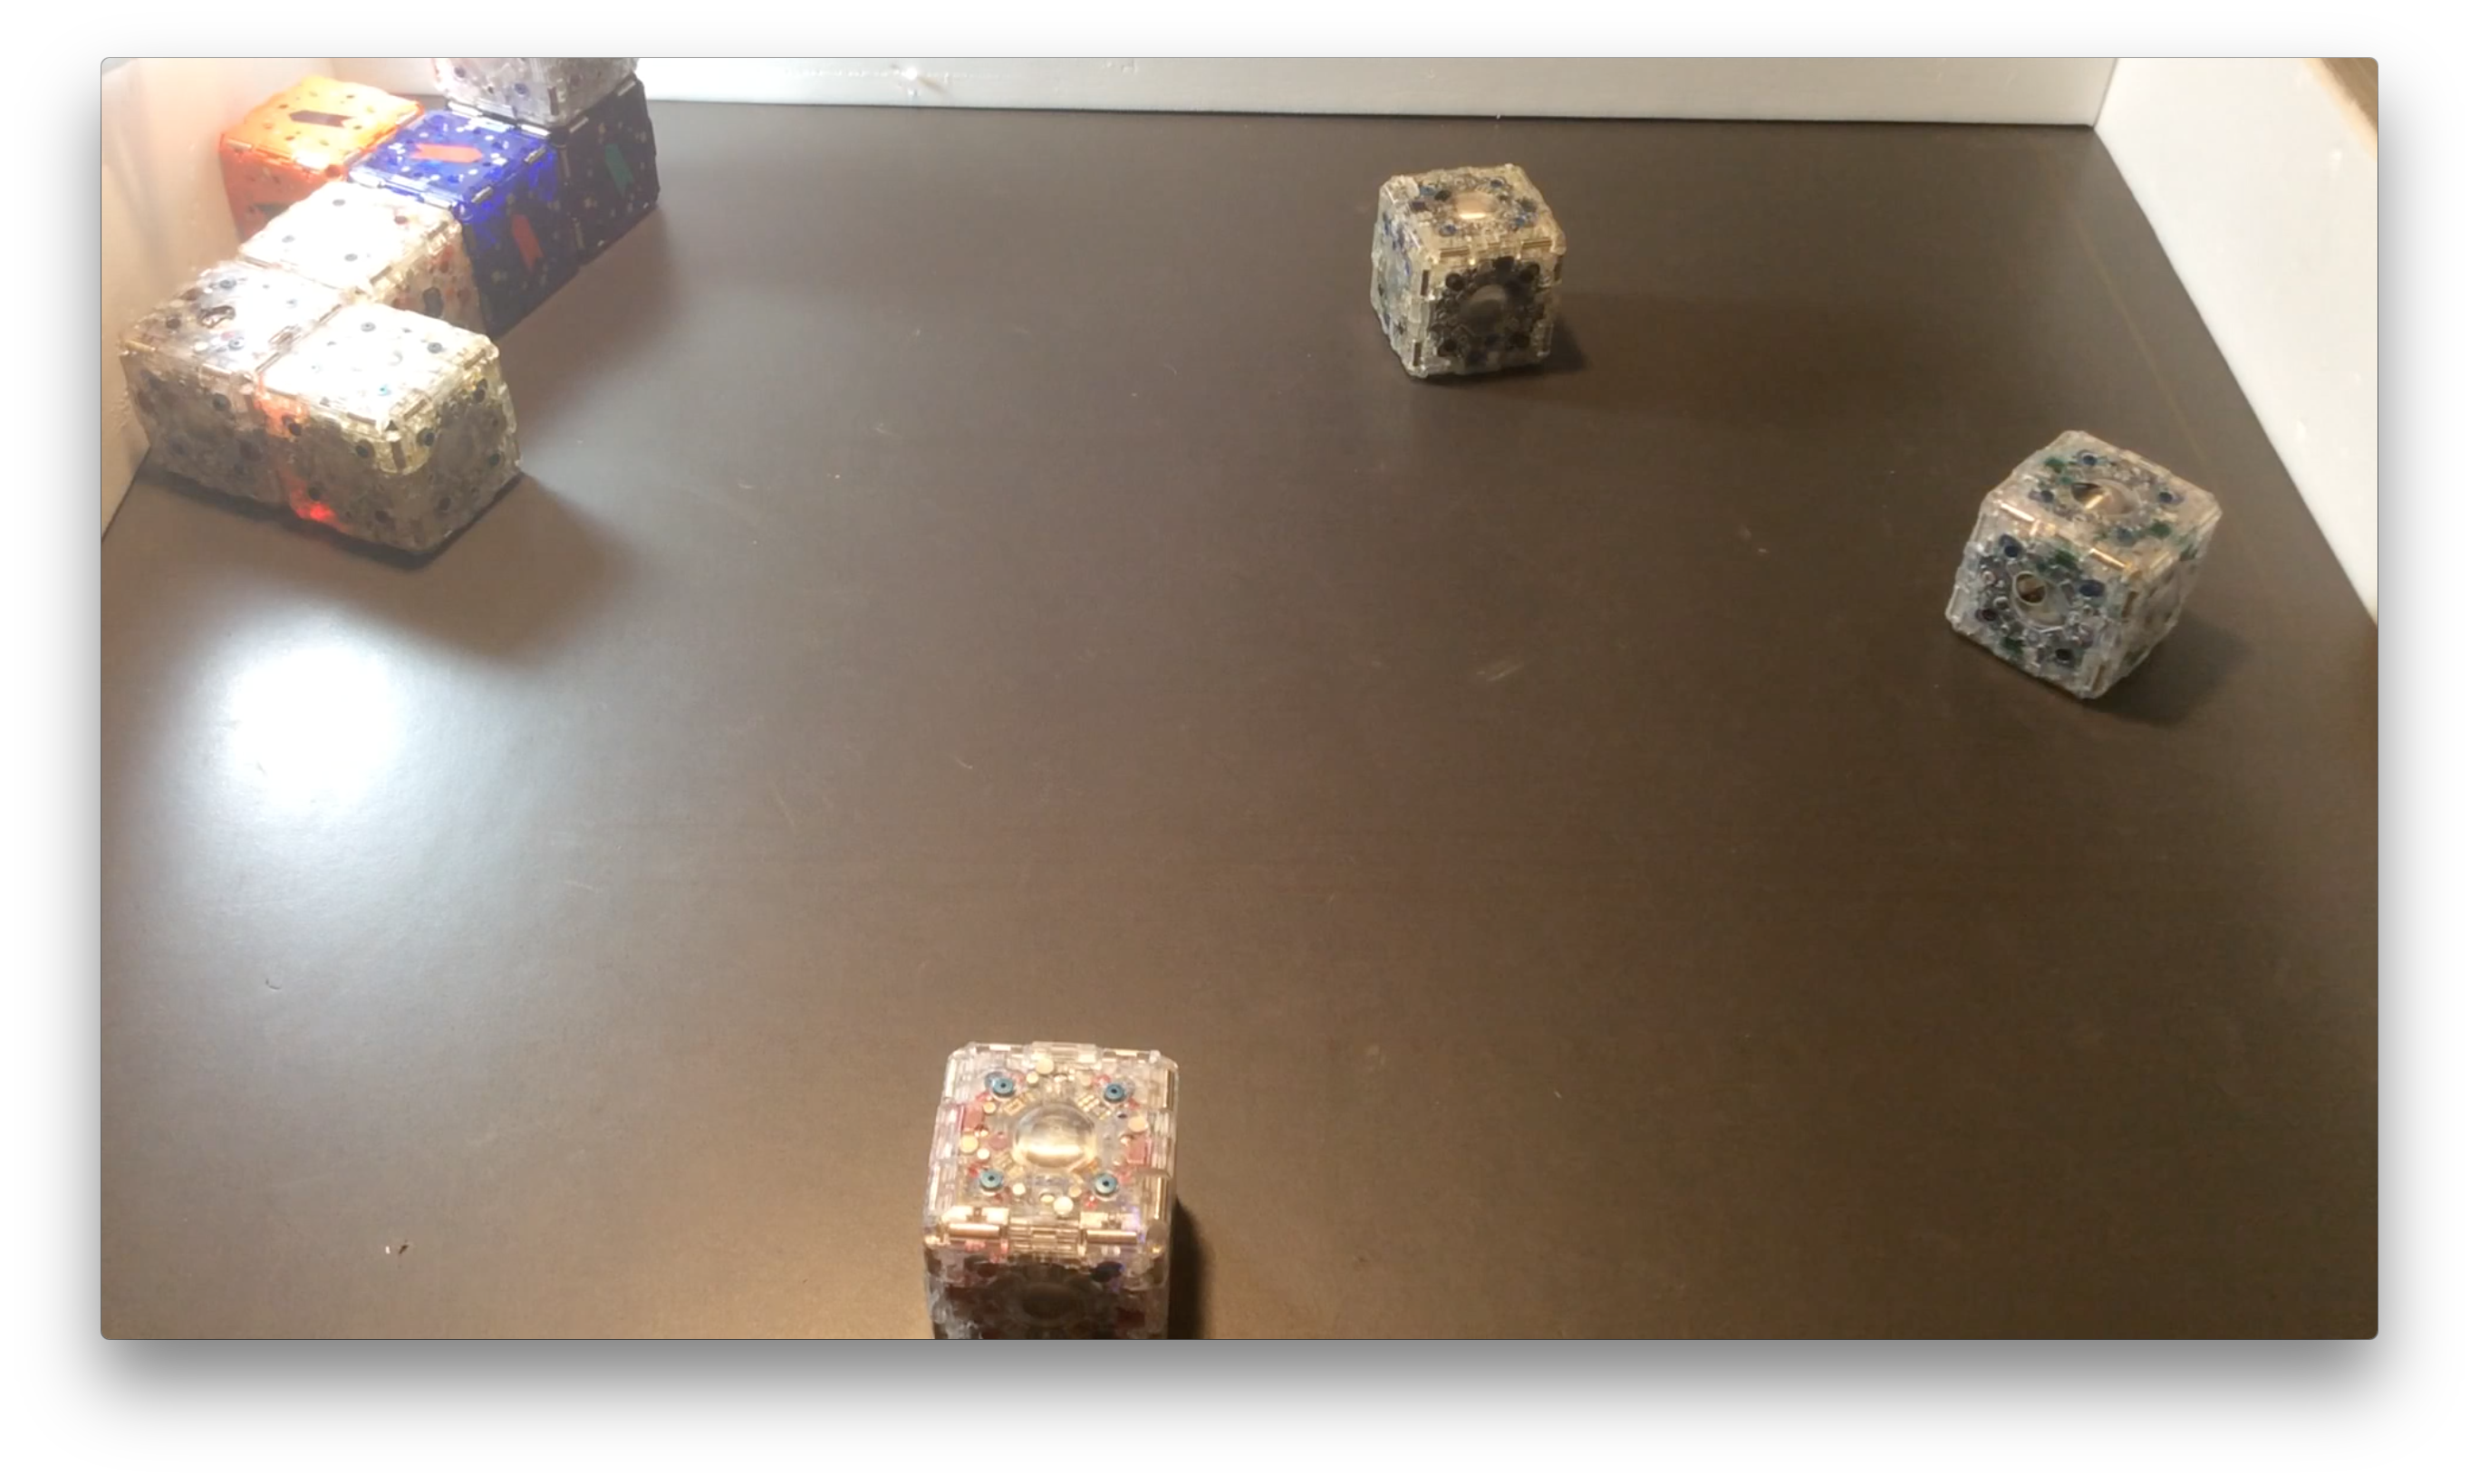
\includegraphics[width = \linewidth]{figures/6-600.png}};
		\node[opacity = 0.5, fill = white, rounded corners] at (-0.5,-0.5) {t = 600 s};
		\end{tikzpicture}
	\end{subfigure}
	
	\caption{This experiment illustrates the light guided aggregation behavior.}
	
	\label{fig:LightExperiment}
\end{figure}


%%%%%%%%%%%%%%%%%%%%%%%%%
\section{Discussion}
\label{sec:Discussion}
%%%%%%%%%%%%%%%%%%%%%%%%%
This paper presents a new magnetic fiducial, the \tagName, for Modular Self-Reconfigurable Robots, and introduces three behaviors which utilize it to accomplish specific tasks.
% The \tagNamePlural~ offers a combination of several features that exist disparately in other MSRR identification technologies.
The \tagNamePlural's use of permanent magnets is inexpensive, functionally simple, and allows for the reading of passive or inactive modules. While other technoligies including NFC tags are also promissing for this application, they are more complex, more expensive (when considering both tags and reader) and are a proprietary standard. %Dusty, hot, and sunlight-exposed environments may be damaging to plastics and readable surfaces in optically based identification systems, and \tagName~ could offer greater robustness in these applications.
One additional advantage of \tagName~ is its scalability in modular robotics applications that involve RF communications. Many magnetic rotary position sensors are immune to stray magnetic fields, and have a very short detection range. A large number of magnet-sensor pairs can be used within a system of many modular robots without any RF interference or confusion. In contrast, RF-based technologies may interfere with one another when densely packed, or interfere with other communications devices in EM-noisy environments including outer space and industrial applications.

The experimental results and behaviors presented in this work are based on preliminary hardware, and have relatively high error rates due to manufacturing and design limitations. Additionally the 3D M-Block robots which this system is tested on has relatively unreliable movement abilities due to electronic and manufacturing problems. However we believe that this system provides justification that this technology could provide a framework that future work could follow to create an effective system to identify the configuration of and control systems with millions of modular elements.

%The behaviors presented in this work are wi applying these behaviors to future systems with millions of modules.

%%%%%%%%%%%%%%%%%%%%%%%%%
\section*{Acknowledgments}
This work is supported by the NSF through grants 1240383 and 1138967.

%%%%%%%%%%%%%%%%%%%%%%%%% 
\section*{Supplementary Material}
\url{http://youtu.be/y27gUFO6mTA}

\bibliographystyle{IEEEtran}

%\bibliography{bibliography-ICRA18.bib}

\bibliography{johnromBibliography2018}

\end{document}
